\documentclass[10pt,openany]{book}
\usepackage{ctex} 
\usepackage{geometry,graphicx,xcolor,color}
\geometry{
  a4paper,
  top=25.4mm, bottom=25.4mm,
  left=20mm, right=20mm,
  headheight=2.17cm,
  headsep=4mm,
  footskip=12mm
}

\usepackage{amssymb,amsmath,mathrsfs}                    % 数学字体
\usepackage{mathpazo}% 采用 Palatino 风格字体
\usepackage[nofontspec]{newpxtext}

\definecolor{winered}{rgb}{0.5,0,0}
\definecolor{structurecolor}{RGB}{122,122,142}
\definecolor{main}{HTML}{3D445F}
\definecolor{second}{HTML}{627581}
\definecolor{third}{HTML}{9D8798}
% 定义引用的颜色
\usepackage{hyperref}
\hypersetup{colorlinks = true, linktoc=all, linkcolor=black, urlcolor=winered}

% ------------------------------------------------------------%
% 定义定理环境
\usepackage{amsthm}
\newtheoremstyle{defstyle}{3pt}{3pt}{\kaishu}{-3pt}{\bfseries\color{main}}{}{0.5em}{\indent 【\thmname{#1} \thmnumber{#2}】 \thmnote{(#3)}}
\newtheoremstyle{thmstyle}{3pt}{3pt}{\kaishu}{-3pt}{\bfseries\color{second}}{}{0.5em}{\indent【\thmname{#1} \thmnumber{#2}】 \thmnote{(#3)}}
\newtheoremstyle{prostyle}{3pt}{3pt}{\kaishu}{-3pt}{\bfseries\color{third}}{}{0.5em}{\indent【\thmname{#1} \thmnumber{#2}】 \thmnote{(#3)}}

\theoremstyle{thmstyle} %theorem style
  \newtheorem{theorem}{定理}[chapter]
\theoremstyle{defstyle} % definition style
  \newtheorem{definition}[theorem]{定义}
  \newtheorem{lemma}[theorem]{引理}
  \newtheorem{corollary}[theorem]{推论}
\theoremstyle{prostyle} % proposition style
  \newtheorem{proposition}[theorem]{命题}
  \newtheorem{example}[theorem]{例题}
  \newtheorem{remark}[theorem]{注}

\renewenvironment{proof}[1][证明]{\par\underline{\textbf{#1.}} \;\fangsong}{\qed\par}
\newenvironment{solution}{\par\underline{\textbf{解.}} \;\kaishu}{\qed\par}
\newcommand{\intro}[1]{\rightline{\parbox[t]{5cm}{\footnotesize \fangsong\quad\quad #1 }}}
% ------------------------------------------------------------%
% ------------------------------------------------------------%
% 设置章形式
\usepackage{titlesec, titletoc}
\linespread{1.2} 				
\usepackage{fancyhdr}
\fancyhf{}
\renewcommand{\headrule}{\color{structurecolor}\hrule width\textwidth}
\pagestyle{fancy}
\renewcommand{\headrulewidth}{1pt}
\fancypagestyle{plain}{\renewcommand{\headrulewidth}{0pt}\fancyhf{}\renewcommand{\headrule}{}}

\fancyhead[c]{\color{structurecolor}\kaishu\rightmark}
\fancyfoot[c]{\color{structurecolor}\small\thepage}

\titleformat{\chapter}[display]{\Large}
{\color{structurecolor}\filleft
\parbox{1cm}{\vbox to 1.5cm{\vfill\hbox to 4cm{\hfill\Huge \bfseries \color{structurecolor}{Chapter} \thechapter \hfill}}}}
{1ex}
{\color{structurecolor} \titlerule[2pt]\large\bfseries \filright \vspace*{1em}}
[\vspace*{1em} {\titlerule[2pt]}]

\titleformat{\section}[frame]{\normalfont\color{structurecolor}}{\footnotesize \enspace \large \textcolor{structurecolor}{\S \,\thesection}\enspace}{6pt}{\Large\filcenter \bf \kaishu }


\titleformat{\subsection}[hang]{\bfseries}{\large\bfseries\color{structurecolor}\thesubsection\enspace}{1pt}{\color{structurecolor}\large\bfseries\filright}

\titleformat{\subsubsection}[hang]{\bfseries}{\large\bfseries\color{structurecolor}\thesubsubsection\enspace}{1pt}{\color{structurecolor}\large\bfseries\filright}
% ------------------------------------------------------------%
% 设置封面
\usepackage{titling}
\renewcommand*{\maketitle}{
    \begin{titlepage}
    \newgeometry{margin = 0in}
    \parindent=0pt
    \vfill
    \begin{center}
        \parbox{0.618\textwidth}{
        \hfill {\bfseries \Huge \thetitle} \\[0.6pt]  
        \rule{0.618\textwidth}{4pt} \\ 
    }
    \end{center}
    \vfill
    \begin{center}
        \parbox{0.618\textwidth}{
        \hfill\Large
        \kaishu 
          \begin{tabular}{r|}
          作者:\theauthor \\ 
          时间:\thedate \\
        \end{tabular}
        }
    \end{center}
    \vfill
    \begin{center}
        \parbox[t]{0.7\textwidth}{\centering \kaishu }
    \end{center}
    \vfill
\end{titlepage}
\restoregeometry
\thispagestyle{empty}
}
% ------------------------------------------------------------%


\title{自用\rm{\LaTeX}书籍模版}
\author{\href{https://www.zhihu.com/people/moment-jue-wang-30}{Jiann}}
\date{\today}

\begin{document}
\frontmatter

\maketitle

\tableofcontents

\mainmatter

\chapter{杂项}
\section{量子散射}

\section{光学定理}
\chapter{数学物理方法}
\section{复变函数}
\chapter{凝聚态场论、量子多体}
\section{LK Formula}
热力学势定义\footnote{a为给定能量、磁场方向动量的电子在k空间的轨道面积,轨道量子化给出:$ a(\varepsilon, \kappa)=(r+\gamma) 2 \pi e H / c h $ }为:$ \Omega=-k T \sum \ln \left(1+\mathrm{e}^{(\zeta-\varepsilon) / k T}\right) $,对能级的求和可以写为:
\begin{equation}
  \Omega=-k T \int_{-\infty}^{\infty} \mathrm{d} \kappa\left(\frac{e H V}{2 \pi^2 c h}\right) \sum_r \ln \left(1+\mathrm{e}^{\left(\zeta-\varepsilon_r\right) / k T}\right)
\end{equation} 
下面考虑一固定的磁场方向动量分量$ \kappa $并取T=0,有:
\begin{equation}\footnote{取T=0的极限,使得对数项中的东西展开}
  \delta \Omega=\delta \kappa\left(\frac{e H V}{2 \pi^2 c h}\right) \sum_{r=0}^n\left(\varepsilon_r-\zeta\right) \equiv D \sum_{r=0}^n\left(\varepsilon_r-\zeta\right)
\end{equation}
对于r的求和,利用Euler-Maclaurin公式,对于整数自变量的函数求和,有如下近似:
\begin{equation}
  \sum_0^n f(r)=\int_0^n f(r) \mathrm{d} r+\frac{1}{2}[f(n)+f(0)]+\frac{1}{12}\left[f^{\prime}(n)-f^{\prime}(0)\right]
  \label{EMF}
\end{equation}
未写出的高阶项为$ o(\frac{1}{n^2}) $,代入以后有:
\begin{equation}
  \begin{aligned}
    \frac{\delta \Omega}{D}= & \int_0^n\left(\varepsilon_r-\zeta\right) \mathrm{d} r+\frac{1}{2}\left(\varepsilon_n-\zeta\right)+\frac{1}{2}\left(\varepsilon_0-\zeta\right) \\
    & +\frac{1}{12}\left[\left(\frac{\partial \varepsilon}{\partial r}\right)_{r=n}-\left(\frac{\partial \varepsilon}{\partial r}\right)_{r=0}\right]
    \end{aligned}
\end{equation}
由于是零温F-D分布,n的定义为满足此式的最大r:$ \varepsilon_r=\zeta $。引入一连续变量x代替$ r+\frac{1}{2} $,定义X为$\varepsilon(X)=\zeta  $ 利用如下偏导数的关系:$ \left(\frac{\partial \varepsilon}{\partial x}\right)_\kappa=\frac{(\partial a / \partial x)_\kappa}{(\partial a / \partial \varepsilon)_\kappa}=\frac{2 \pi e H / c h}{2 \pi m / \hbar^2}=\beta H $,
将上述的积分改变变量,并取出与量子震荡有关的那项,有\footnote{此项没有对x的积分,因此是只和费米面处的态有关}:
\begin{equation}
  \delta \tilde{\Omega}=\delta \kappa \frac{e \beta H^2 V}{4 \pi^2 c h}\left\{\left[X-\left(n+\frac{1}{2}\right)\right]^2-\left[\left(X-\left(n+\frac{1}{2}\right)\right]+\frac{1}{6}\right\}\right.
\end{equation}  
上式对于$ \left(n+\frac{1}{2}\right) \leqslant X \leqslant\left(n+\frac{3}{2}\right) $成立,当X超出这个定义域时,n随之改变,最终是关于X的一个周期函数,对其做傅立叶变换有:
\begin{equation}
  \delta \tilde{\Omega}=\frac{\delta \kappa e \beta H^2 V}{4 \pi^2 c h} \sum_{p=1}^{\infty} \frac{1}{\pi^2 p^2} \cos 2 \pi p\left(X-\frac{1}{2}\right)
\end{equation} 
对$ \kappa $积分,给出:
\begin{equation}
  \tilde{\Omega}=\frac{e H^2 V}{4 \pi^2 c h} \int \beta \mathrm{d} \kappa \sum_{p=1}^{\infty} \frac{1}{\pi^2 p^2} \cos \left\{2 \pi p\left[X(\kappa)-\frac{1}{2}\right]\right\}
\end{equation} 
$ \kappa $的积分上限为与费米面相切的最大$ \kappa $,但一般将其取为无穷作为一种好的近似。将X作为$ \kappa $的函数在$ \kappa=0 $处做展开,并只保留到二阶项\footnote{假设X为偶函数},有:
\begin{equation}
  \begin{aligned}
    I_p & =\int_{-\infty}^{\infty} \mathrm{d} \kappa \cos \left[2 \pi p\left(X(\kappa)-\frac{1}{2}\right)\right] \\
    & =2 \int_0^{\infty} \mathrm{d} \kappa \cos \left[2 \pi p\left(X_0 \pm \frac{1}{2} X^{\prime \prime} \kappa^2-\frac{1}{2}\right)\right]\\
    & =\left(p X^{\prime \prime}\right)^{-1 / 2} \cos \left[2 \pi p\left(X_0-\frac{1}{2}\right) \pm \frac{1}{4} \pi\right]
  \end{aligned}
\end{equation}  
对傅立叶频率p求和,有:
\begin{equation}
  \tilde{\Omega}=\left(\frac{e}{2 \pi c h}\right)^{3 / 2} \frac{\beta H^{5 / 2}}{\pi^2\left(A^{\prime \prime}\right)^{1 / 2}} \sum_{p=1}^{\infty} \frac{1}{p^{5 / 2}} \cos \left[2 \pi p\left(\frac{F}{H}-\frac{1}{2}\right) \pm \frac{\pi}{4}\right]
  \label{LKF}
\end{equation}  
其中引入了记号:$ F=(c h / 2 \pi e) A=X_0 H ,A^{\prime \prime}=\left|\partial^2 \mathscr{A} / \partial \kappa^2\right|_{\kappa=0}=(2 \pi e H / c h) X^{\prime \prime}$
上面的内容忽视了有限温度、电子弛豫时间、电子自旋以及外加磁场和样品的不均匀性。上述内容都可以被“相位涂抹”所描述。这是因为
上述效应都可以等价\eqref{LKF}中不同F的叠加,这也等价于额外的一个相位因子。\\

记$ \psi=2 \pi p\left(\frac{F}{H}-\frac{1}{2}\right) \pm \frac{\pi}{4} $,不同F的叠加可以等效为对积分中的$ \cos(\psi) $作如下替换:
\begin{equation}
  \begin{aligned}
    I&=\int_{-\infty}^{\infty} \cos (\psi+\phi) D(\phi / \lambda) \mathrm{d} \phi / \int_{-\infty}^{\infty} D(\phi / \lambda) \mathrm{d} \phi\\
    &=\mathscr{R} \mathrm{e}^{\mathrm{i} \psi} \int_{-\infty}^{\infty} \mathrm{e}^{\mathrm{i} \phi} D(\phi / \lambda) \mathrm{d} \phi / \int_{-\infty}^{\infty} D(\phi / \lambda) \mathrm{d} \phi\\
    &=\mathscr{R} \mathrm{e}^{\mathrm{i} \psi} \int_{-\infty}^{\infty} \mathrm{e}^{\mathrm{i} \lambda z} D(z) \mathrm{d} z / \int_{-\infty}^{\infty} D(z) \mathrm{d} z\\
    &=\mathscr{R}\left\{[f(\lambda) / f(0)] \mathrm{e}^{\mathrm{i} \psi}\right\}
  \end{aligned}
\end{equation}
其中引入了$ z=\phi / \lambda,f(\lambda)=\int_{-\infty}^{\infty} \mathrm{e}^{\mathrm{i} \lambda z} D(z) \mathrm{d} z $。\\

因此,“相位涂抹”相当于引入了一个振幅缩小因子:$ R=|f(\lambda)| / f(0) $,同时改变相位。当$ D(z) $作为z的函数是一个对称函数时,$ f(\lambda) $是实的,此时没有相位改变。\\

有限温度时的F-D分布可以看作一系列化学势不同的金属的零温分布函数的叠加,这点将在之后更形式化地说明。分布函数可以写为:
\begin{equation}
  -\frac{\mathrm{d} f(\mu)}{\mathrm{d} \mu}=\frac{1}{2 k T[1+\cosh (\mu-\zeta) / k T]}
\end{equation}
这个因子最终对应于一个系数:$ R_T=\frac{\pi \lambda}{\sinh \pi \lambda}=\frac{2 \pi^2 p k T / \beta H}{\sinh \left(2 \pi^2 p k T / \beta H\right)} $。
当自变量远远大于1时,有$ R_T=\frac{4 \pi^2 p k T}{\beta H} \exp \left(-2 \pi^2 p k T / \beta H\right) $。\\

如果电子具有有限的弛豫时间,由于散射,尖锐的量子能级将被扩展,同时也导致一个振幅因子,称为Dingle因子。能级的扩展可以被一Lorentzian分布描述,此时能级在
$\epsilon\sim\epsilon+d\epsilon  $处的概率为:$ \frac{d\epsilon}{(\epsilon-\epsilon_r)^2+(h/2\tau)^2} $。如果$ \tau $与能级无关,则能级
扩展和费米能$ \mu $在它的真实值$ \zeta $附近的延展等效。这带来的“相位涂抹”给出因子:
\begin{equation}
  R_{\mathrm{D}}=\mathrm{e}^{-\pi p h / \beta H \tau}=\mathrm{e}^{-\pi p / \omega_{\mathrm{c}} \tau}
\end{equation}     
可以定义一个特征温度Dingle温度,使得上面的因子和有限温度导致的因子具有相似的形式:
\begin{equation}
  R_{\mathrm{D}}=\exp \left(-2 \pi^2 p k x / \beta H\right)
\end{equation}
其中$  x=\hbar / 2 \pi k \tau$是Dingle温度。
\section{量子可积与Bethe拟设}
\section{随机势场下的电子气}
\subsubsection*{外场下的无相互作用电子}
考虑一个外场下的无相互作用电子体系,哈密顿量为:
\begin{equation}
  H=H_0+V=\sum_\sigma \int d \mathbf{r} \Psi_\sigma^{\dagger}(\mathbf{r}) H_0(\mathbf{r}) \Psi_\sigma(\mathbf{r})+\sum_\sigma \int d \mathbf{r} \Psi_\sigma^{\dagger}(\mathbf{r}) V_\sigma(\mathbf{r}) \Psi_\sigma(\mathbf{r})
\end{equation}
照旧假设$ H_0 $是可解的,它的本征值、本征态以及格林函数也知道,现在研究Exact虚时传播子$ \mathcal{G}(b, a)=-\left\langle T_\tau \Psi(b) \Psi^{\dagger}(a)\right\rangle $。其中
每个字母指标指代空间位置、虚时和自旋指标。仍有戴森方程以及它的迭代展开。  
\begin{equation}
  \mathcal{G}(b, a)=\mathcal{G}^0(b, a)+\int d 1 \mathcal{G}(b, 1) V(1) \mathcal{G}^0(1, a)
  \label{Daysoneq}
\end{equation}
由于外场是静止的,哈密顿量不含时,格林函数只依赖于时间差,可用松原频率做傅立叶展开,由此有:
\begin{equation}
  \mathcal{G}\left(\mathbf{r}_b, \mathbf{r}_a ; i k_n\right)=\mathcal{G}^0\left(\mathbf{r}_b, \mathbf{r}_a ; i k_n\right)+\int d \mathbf{r}_1 \mathcal{G}^0\left(\mathbf{r}_b, \mathbf{r}_1 ; i k_n\right) V(1) \mathcal{G}\left(\mathbf{r}_1, \mathbf{r}_a ; i k_n\right)
\end{equation}
将格林函数在$ H_0 $的本征态表象下写出是方便的\footnote{对于自由电子就是动量表象},由此定义:
\begin{equation}
  \mathcal{G}_{\nu \nu^{\prime}} \equiv \int d \mathbf{r} d \mathbf{r}^{\prime}\langle\nu \mid \mathbf{r}\rangle \mathcal{G}\left(\mathbf{r}, \mathbf{r}^{\prime}\right)\left\langle\mathbf{r}^{\prime} \mid \nu^{\prime}\right\rangle \quad \Leftrightarrow \quad \mathcal{G}\left(\mathbf{r}, \mathbf{r}^{\prime}\right)=\sum_{\nu \nu^{\prime}}\langle\mathbf{r} \mid \nu\rangle \mathcal{G}_{\nu \nu^{\prime}}\left\langle\nu^{\prime} \mid \mathbf{r}^{\prime}\right\rangle
\end{equation} 
此时裸格林函数可以直接写出:$ \mathcal{G}_{\nu, \nu^{\prime}}^0\left(i k_n\right)=\frac{1}{i k_n-\xi_\nu} \delta_{\nu, \nu^{\prime}} $,此时戴森方程可以从积分方程变为矩阵方程:
\begin{equation}
  \mathcal{G}\left(\nu_b \nu_a ; i k_n\right)=\delta_{\nu_b, \nu_a} \mathcal{G}^0\left(\nu_a \nu_a ; i k_n\right)+\sum_{\nu_c} \mathcal{G}^0\left(\nu_b \nu_b ; i k_n\right) V_{\nu_b \nu_c} \mathcal{G}\left(\nu_c \nu_a ; i k_n\right)
\end{equation} 
\begin{figure}[htp]
  \centering
  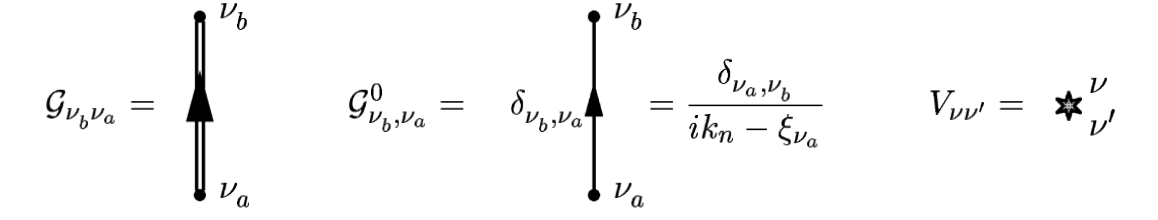
\includegraphics[scale=0.7]{biaoji.png}
  \caption{自能定义}
\end{figure}
戴森方程的图表示为:
\begin{figure}[htbp]
  \centering
  \includegraphics*[scale=0.7]{DaysonEq.png}
  \caption{戴森方程}
\end{figure}
\subsubsection*{杂质导致的随机势}
现在考虑杂质导致的随机势下的无相互作用电子体系,外场可以写为:
\begin{equation}
  V(\mathbf{r})=\sum_{j=1}^{N_{\mathrm{imp}}} u\left(\mathbf{r}-\mathbf{P}_j\right), \quad \mathbf{P}_j \text { is randomly distributed. }
\end{equation}
在此假设杂质密度远低于电子密度,且u是一个弱且短程的势能\footnote{弱意味着势能远小于能级间隙}。此时戴森展开的第n阶项为:
\begin{equation}
  \begin{aligned}
    \mathcal{G}^{(n)}\left(\mathbf{r}_b, \mathbf{r}_a\right)= & \sum_{j_1}^{N_{\mathrm{imp}}} \ldots \sum_{j_n}^{N_{\mathrm{imp}}} \int d \mathbf{r}_1 \ldots \int d \mathbf{r}_n \\
    & \times \mathcal{G}^0\left(\mathbf{r}_b-\mathbf{r}_n\right) u\left(\mathbf{r}_n-\mathbf{P}_{j_n}\right) \ldots u\left(\mathbf{r}_2-\mathbf{P}_{j_2}\right) \mathcal{G}^0\left(\mathbf{r}_2-\mathbf{r}_1\right) u\left(\mathbf{r}_1-\mathbf{P}_{j_1}\right) \mathcal{G}^0\left(\mathbf{r}_1-\mathbf{r}_a\right)
    \end{aligned}
\end{equation}
严格求解上述方程是没有希望的,但之后可以看到,在取平均以后上述方程有很好的性质。对于方程右式做傅立叶变换,有:
\begin{equation}
  \begin{aligned}
    \mathcal{G}^{(n)}\left(\mathbf{r}_b, \mathbf{r}_a\right)= & \sum_{j_1 \ldots j_n}^{N_{\mathrm{imp}}} \frac{1}{\mathcal{V}^n} \sum_{\mathbf{q}_1 \ldots \mathbf{q}_n} \frac{1}{\mathcal{V}^2} \sum_{\mathbf{k}_a \mathbf{k}_b} \frac{1}{\mathcal{V}^{n-1}} \sum_{\mathbf{k}_1 \ldots \mathbf{k}_{n-1}} \int d \mathbf{r}_1 \ldots \int d \mathbf{r}_n \\
    & \times \mathcal{G}_{\mathbf{k}_b}^0 u_{\mathbf{q}_n} \mathcal{G}_{\mathbf{k}_{n-1}}^0 u_{\mathbf{q}_{n-1}} \ldots u_{\mathbf{q}_2} \mathcal{G}_{\mathbf{k}_1}^0 u_{\mathbf{q}_1} \mathcal{G}_{\mathbf{k}_a}^0 e^{-i\left(\mathbf{q}_n \cdot \mathbf{P}_{j_n}+\ldots+\mathbf{q}_2 \cdot \mathbf{P}_{j_2}+\mathbf{q}_1 \cdot \mathbf{P}_{j_1}\right)} \\
    & \times e^{i \mathbf{k}_b \cdot\left(\mathbf{r}_b-\mathbf{r}_n\right)} e^{i \mathbf{q}_n \cdot \mathbf{r}_n} e^{i \mathbf{k}_{n-1} \cdot\left(\mathbf{r}_n-\mathbf{r}_{n-1}\right)} \ldots e^{i \mathbf{q}_2 \cdot \mathbf{r}_2} e^{i \mathbf{k}_1 \cdot\left(\mathbf{r}_2-\mathbf{r}_1\right)} e^{i \mathbf{q}_1 \cdot \mathbf{r}_1} e^{i \mathbf{k}_a \cdot\left(\mathbf{r}_1-\mathbf{r}_a\right)}
    \end{aligned}
\end{equation}
利用空间积分给出的delta函数,再对左式也做傅立叶变换,可以化简为:
\begin{equation}
  \begin{aligned}
    \mathcal{G}_{\mathbf{k}_b \mathbf{k}_a}^{(n)}= & \sum_{j_1 \ldots j_n}^{N_{\text {imp }}} \frac{1}{\mathcal{V}^{n-1}} \sum_{\mathbf{k}_1 \ldots \mathbf{k}_{n-1}} e^{-i\left[\left(\mathbf{k}_b-\mathbf{k}_{n-1}\right) \cdot \mathbf{P}_{j_n}+\ldots+\left(\mathbf{k}_1-\mathbf{k}_a\right) \cdot \mathbf{P}_{j_1}\right]} \\
    & \times \mathcal{G}_{\mathbf{k}_b}^0 u_{\mathbf{k}_b-\mathbf{k}_{n-1}} \mathcal{G}_{\mathbf{k}_{n-1}}^0 \cdots u_{\mathbf{k}_2-\mathbf{k}_1} \mathcal{G}_{\mathbf{k}_1}^0 \cdots u_{\mathbf{k}_1-\mathbf{k}_a} \mathcal{G}_{\mathbf{k}_a}^0 .
    \end{aligned}
\end{equation}
可以看出,动量为k的粒子每次被散射以后动量都将发生改变,在引入新的假设前这无法被化简。
\subsubsection*{杂质自平均}
对杂质场的求平均数学上需要对N个辅助体系都算出来再求平均,某些情况下等价于对杂质位置求平均:
\begin{equation}
  \frac{1}{\mathcal{V}}\left\langle\mathcal{G}_{\mathbf{k}_b \mathbf{k}_a}\right\rangle_{\mathrm{imp}} \equiv \delta_{\mathbf{k}_b, \mathbf{k}_a} \overline{\mathcal{G}}_{\mathbf{k}_a} \equiv \frac{\delta_{\mathbf{k}_b, \mathbf{k}_a}}{N_{\mathrm{sys}}} \sum_{i=1}^{N_{\mathrm{sys}}} \mathcal{G}_{\mathbf{k}_a}^{\mathrm{sys}_{\mathrm{i}}} \sim \delta_{\mathbf{k}_b, \mathbf{k}_a} \frac{1}{\mathcal{V}} \int d \mathbf{P}_1 \frac{1}{\mathcal{V}} \int d \mathbf{P}_2 \cdots \frac{1}{\mathcal{V}} \int d \mathbf{P}_{N_{\mathrm{imp}}} \mathcal{G}_{\mathbf{k}_a}
\end{equation}
需要注意到,戴森级数中的第n项包含n次散射,但其中的一些散射过程可能发生在同一点。由于假设杂质密度低,对于一个杂质的散射为Leading oder,其次是两个杂质的散射。由此
将求和拆解:
\begin{equation}
  \begin{aligned}
    & \sum_{j_1, \ldots, j_n}^{N_{\mathrm{imp}}} e^{i \sum_{l=1}^n \mathbf{q}_l \cdot \mathbf{P}_{j_l}}=\sum_{h_1}^{N_{\mathrm{imp}}} e^{i\left(\sum_{\mathbf{q}_{j_1} \in Q} \mathbf{q}_{j_1}\right) \cdot \mathbf{P}_{h_1}} \\
    & +\sum_{Q_1 \cup Q_2=Q} \sum_{h_1}^{N_{\mathrm{imp}}} \sum_{h_2}^{N_{\mathrm{imp}}} e^{i\left(\sum_{\mathbf{q}_{l_1} \in Q_1} \mathbf{q}_{l_1}\right) \cdot \mathbf{P}_{h_1}} e^{i\left(\sum_{\mathbf{q}_{l_2} \in Q_2} \mathbf{q}_{l_2}\right) \cdot \mathbf{P}_{h_2}} \\
    & +\sum_{Q_1 \cup Q_2 \cup Q_3=Q} \sum_{h_1}^{N_{\mathrm{imp}}} \sum_{h_2}^{N_{\mathrm{imp}}} \sum_{h_3}^{N_{\mathrm{imp}}} e^{i\left(\sum_{\mathbf{q}_{l_1} \in Q_1} \mathbf{q}_{l_1}\right) \cdot \mathbf{P}_{h_1}} e^{i\left(\sum_{\mathbf{q}_{l_2} \in Q_2} \mathbf{q}_{l_2}\right) \cdot \mathbf{P}_{h_2}} e^{i\left(\sum_{\mathbf{q}_{l_3} \in Q_3} \mathbf{q}_{l_3}\right) \cdot \mathbf{P}_{h_h}}\\
    & +\ldots
    \end{aligned}
\end{equation}
其中$ Q=\left\{\mathbf{q}_1, \mathbf{q}_2, \ldots, \mathbf{q}_n\right\} $为n个散射波矢。所有在同一子集$ Q_i $中的波矢都被同一杂质散射。\footnote{严格来说同一点中不能有多个杂质,上述求和之间相互没有限制,会引入$ 1 / N_{\mathrm{imp}} $阶的误差 }\\

可以预想到,在求平均以后,平移不变性恢复,对同一点杂质的散射动量守恒。每个指数因子的平均给出一个delta函数:
\begin{equation}
  \left\langle e^{i\left(\sum_{\mathbf{q}_{h_i} \in Q_i} \mathbf{q}_{h_i}\right) \cdot \mathbf{P}_{h_i}}\right\rangle_{\mathrm{imp}}=\frac{1}{\mathcal{V}} \int d \mathbf{P}_{h_i} e^{i\left(\sum_{\mathbf{q}_{h_i} \in Q_h} \mathbf{q}_{h_i}\right) \cdot \mathbf{P}_{h_i}}=\delta_{0, \sum_{\mathbf{q}_{h_i} \in Q_h} \mathbf{q}_{h_i}} .
\end{equation}
对于n阶戴森级数展开的平均有:
\begin{equation}
  \begin{aligned}
    \left\langle\mathcal{G}_{\mathbf{k}}^{(n)}\right\rangle_{\mathrm{imp}}= & \frac{1}{\mathcal{V}^{n-1}} \sum_{\mathbf{k}_1 \ldots \mathbf{k}_{n-1}} \sum_{p=1}^n \sum_{\bigcup_{h=1}^p Q_h=Q} \prod_{h=1}^p\left(N_{\mathrm{imp}} \delta_{0, \Sigma_{Q_h}\left(\mathbf{k}_{h_i}-\mathbf{k}_{\left(h_i-1\right)}\right)}\right) \\
    & \times \mathcal{G}_{\mathbf{k}}^0 u_{\mathbf{k}-\mathbf{k}_1} \mathcal{G}_{\mathbf{k}_1}^0 u_{\mathbf{k}_1-\mathbf{k}_2} \mathcal{G}_{\mathbf{k}_2}^0 \ldots u_{\mathbf{k}_{n-1}-\mathbf{k}} \mathcal{G}_{\mathbf{k}}^0 .
    \end{aligned}
\end{equation}
由于每个杂质给出一个delta函数,因此还剩下n-1-p个动量求和,剩下的p个体积倒数同$ N_{imp} $组成杂质密度,因此图中每个杂质贡献一个杂质密度。
\subsubsection*{被杂质散射的电子的自能}
自能定义为传播子中的所有单粒子不可约图的求和,并去掉两端的格林函数。
\begin{figure}[htbp]
  \centering
  \includegraphics*[scale=0.7]{selfenergy.png}
  \caption{<caption>}
  \label{<label>}
\end{figure}
通过形式上的等比级数求和,可以将完整格林函数用裸格林函数与自能表示出:
\begin{equation}
  \left\langle\mathcal{G}_{\mathbf{k}}\left(i k_n\right)\right\rangle_{\mathrm{imp}}=\frac{\mathcal{G}_{\mathbf{k}}^0}{1-\mathcal{G}_{\mathbf{k}}^0 \Sigma_{\mathbf{k}}}=\frac{1}{\left(\mathcal{G}_{\mathbf{k}}^0\right)^{-1}-\Sigma_{\mathbf{k}}}=\frac{1}{i k_n-\xi_{\mathbf{k}}-\Sigma_{\mathbf{k}}\left(i k_n\right)}
\end{equation}
求解格林函数的问题现在转换为求解自能,下面对自能进行逐级近似。\\

最低阶的近似是只考虑单点、单次的散射过程:$ \Sigma_{\mathbf{k}}^{\mathrm{LOA}}\left(i k_n\right) \equiv n_{\mathrm{imp}} u_0=n_{\mathrm{imp}} \int d \mathbf{r} u(\mathbf{r}), $,这只是将激发的能量平移了一个常数,可以通过平移化学势使得这种项没有贡献。
\subsection*{一阶玻恩近似}
现在自能图只考虑单个杂质散射两次\footnote{模方来自u(r)是个实函数,它的傅立叶变换正负部分互为共轭}:
\begin{equation}
  \Sigma_{\mathbf{k}}^{1 \mathrm{BA}}\left(i k_n\right) \equiv n_{\mathrm{imp}} \sum_{\mathbf{k}^{\prime}}\left|u_{\mathbf{k}-\mathbf{k}^{\prime}}\right|^2 \frac{1}{i k_n-\xi_{\mathbf{k}^{\prime}}}
\end{equation}
此时的自能是个复数,这使得完全格林函数的极点从实轴上移到复平面上,由此具有有限寿命。将自能的自变量延拓到实轴,有\footnote{其中用到了delta函数的另一种形式:$ \delta(x)=\lim _{\varepsilon \rightarrow 0} \frac{1}{\pi} \frac{\varepsilon}{\varepsilon^2+x^2} . $ }:
\begin{equation}
  \begin{aligned}
    \Sigma_{\mathbf{k}}^{1 \mathrm{BA}}\left(\omega+i \operatorname{sgn}\left(k_n\right) \eta\right) & =n_{\mathrm{imp}} \sum_{\mathbf{k}^{\prime}}\left|u_{\mathbf{k}-\mathbf{k}^{\prime}}\right|^2 \frac{1}{\left(\omega-\xi_{\mathbf{k}^{\prime}}\right)+i \operatorname{sgn}\left(k_n\right) \eta} \\
    & =\sum_{\mathbf{k}^{\prime}} n_{\mathrm{imp}}\left|u_{\mathbf{k}-\mathbf{k}^{\prime}}\right|^2\left[\frac{\omega-\xi_{\mathbf{k}^{\prime}}}{\left(\omega-\xi_{\mathbf{k}^{\prime}}\right)^2+\eta^2}-i \operatorname{sgn}\left(k_n\right) \pi \delta\left(\omega-\xi_{\mathbf{k}^{\prime}}\right)\right] .
    \end{aligned}
\end{equation}
由于考虑的情况中温度总是远小于费米能,我们关注费米面附近的激发,即考虑如下范围:
\begin{equation}
  |\mathbf{k}| \sim k_{\mathrm{F}} \quad \text { and } \quad\left|i k_n \rightarrow \omega+i \operatorname{sgn}\left(k_n\right) \eta\right| \ll \varepsilon_{\mathrm{F}} .
\end{equation}
由于电子的重分布将屏蔽杂质带来的额外电荷,$ u_k $可以看作一个上述区间内变化较慢的函数,可以得到,自能的实部趋近于零,剩下一个虚部:
\begin{equation}
  \Sigma_{\mathbf{k}}^{1 \mathrm{BA}}\left(i k_n\right)=-i \pi \operatorname{sgn}\left(k_n\right) \sum_{\mathbf{k}^{\prime}} n_{\text {imp }}\left|u_{\mathbf{k}-\mathbf{k}^{\prime}}\right|^2 \delta\left(\xi_{\mathbf{k}}-\xi_{\mathbf{k}^{\prime}}\right)=-i \operatorname{sgn}\left(k_n\right) \frac{1}{2 \tau_{\mathbf{k}}},
\end{equation} 
上面引入了杂质散射时间:$ \frac{1}{\tau_{\mathbf{k}}} \equiv 2 \pi \sum_{\mathbf{k}^{\prime}} n_{\mathrm{imp}}\left|u_{\mathbf{k}-\mathbf{k}^{\prime}}\right|^2 \delta\left(\xi_{\mathbf{k}}-\xi_{\mathbf{k}^{\prime}}\right) $。由此可以得到完全格林函数,并延拓到复平面:
\begin{equation}
  \mathcal{G}_{\mathbf{k}}^{1 \mathrm{BA}}\left(i k_n\right)=\frac{1}{i k_n-\xi_{\mathbf{k}}+i \frac{\operatorname{sgn}\left(k_n\right)}{2 \tau_{\mathbf{k}}}} \underset{i k_n \rightarrow z}{\longrightarrow} \mathcal{G}_{\mathbf{k}}^{1 \mathrm{BA}}(z)=\left\{\begin{array}{l}
    \frac{1}{z-\xi_{\mathbf{k}}+\frac{i}{2 \tau_{\mathbf{k}}}}, \operatorname{Im} z>0 \\
    \frac{1}{z-\xi_{\mathbf{k}}-\frac{i}{2 \tau_{\mathbf{k}}}}, \operatorname{Im} z<0 .
    \end{array}\right.	
\end{equation} 
计算时域以及位置空间的格林函数可以看到,一阶玻恩近似的自能项中包含的虚部,使得传播子在时间和空间上都指数衰减。
\subsection*{完全玻恩近似}
完全玻恩近似是指考虑含有一个杂质散射的所有图,这在$ n_{imp} $阶是完全的,此时自能的图表示为:
\begin{figure}[htbp]
  \centering
  \includegraphics*[scale=0.7]{FBASE.png}
  \caption{完全玻恩近似的自能图表示}
\end{figure} 
引入转移矩阵,图表示为:
\begin{figure}[htbp]
  \centering
  \includegraphics*[scale=0.7]{tmatrix.png}
  \caption{t矩阵的图表示}
\end{figure}
可以看出自能就是t矩阵的对角元。仍只考虑费米面附近的电子,此时t矩阵的实部近似为常数,可以被重定义化学式抵消,而虚部可以利用光学定理\footnote{由图表示可得到矩阵方程:$ t=u+u \mathcal{G}^0 t $。由于u是厄米矩阵,同时求厄米共轭再代回有:$ t=u+\left(t^{\dagger} \mathcal{G}^0 t-t^{\dagger}\left(\mathcal{G}^0\right)^{\dagger} u \mathcal{G}^0 t\right) $,只有中间
一项是非厄米的,因此虚部全部来自于它:$ \operatorname{Im} t_{\mathbf{k}, \mathbf{k}}=\operatorname{Im}\left\langle\mathbf{k}\left|t^{\dagger} \mathcal{G}^0 t\right| \mathbf{k}\right\rangle=\operatorname{Im} \sum_{\mathbf{k}^{\prime}} t_{\mathbf{k}, \mathbf{k}^{\prime}}^{\dagger} \mathcal{G}_{\mathbf{k}^{\prime}}^0 t_{\mathbf{k}^{\prime}, \mathbf{k}} $   }:
\begin{equation}
  \begin{aligned}
    & \operatorname{Im} \Sigma_{\mathbf{k}}^{\mathrm{FBA}}\left(i k_n\right)= \operatorname{Im} t_{\mathbf{k}, \mathbf{k}}\left(i k_n\right)=\operatorname{Im} \sum_{\mathbf{k}^{\prime}} \frac{\left|t_{\mathbf{k}, \mathbf{k}^{\prime}}\right|^2}{i k_n-\xi_{\mathbf{k}^{\prime}}} \\
    & \underset{i k_n \rightarrow \omega+i \operatorname{sgn}\left(k_n\right) \eta}{\longrightarrow}-\operatorname{sgn}\left(k_n\right) \pi \sum_{\mathbf{k}^{\prime}}\left|t_{\mathbf{k}, \mathbf{k}^{\prime}}\right|^2 \delta\left(\omega-\xi_{\mathbf{k}^{\prime}}\right) .
    \end{aligned}
  \label{fba}
\end{equation}
可以看到,它和一阶玻恩近似的虚部长的差不多,只不过$ n_{\mathrm{imp}}\left|u_{\mathbf{k}-\mathbf{k}^{\prime}}\right|^2\to\left|t_{\mathbf{k}, \mathbf{k}^{\prime}}\right|^2 $。
\subsection*{自洽玻恩近似} 
通过将裸传播子换位全传播子,可得到一个自洽方程,若仍只考虑单杂质散射,就是自洽玻恩近似,此时的自能或者是转移矩阵的对角元为:
\begin{equation}
  t_{\mathbf{k}}^{\mathrm{SCBA}} \equiv n_{\mathrm{imp}}\left[u_0 \delta_{\mathbf{k}, \mathbf{k}}+\sum_{\mathbf{k}^{\prime}} u_{\mathbf{k}-\mathbf{k}^{\prime}} \mathcal{G}_{\mathbf{k}^{\prime}} t_{\mathbf{k}^{\prime}, \mathbf{k}}\right]
\end{equation}
由于相同的论述,实部可以略去,关注虚部:
\begin{equation}
  \Sigma_{\mathbf{k}}^i=\operatorname{Im} \sum_{\mathbf{k}^{\prime}} \frac{\left|t_{\mathbf{k}, \mathbf{k}^{\prime}}^{\mathrm{SCBA}}\right|^2}{i k_n-\xi_{\mathbf{k}^{\prime}}-i \Sigma_{\mathbf{k}^{\prime}}^i}
\end{equation}
它与\eqref{fba}不同点在于使用的是上述自洽方程给出的转移矩阵。最终求和的图中不包括带交叉的图,因为我们总考虑费米面附近的动量,带交叉的图积分的动量空间总比不带交叉的图小。
\subsection*{一些评注}
这一节内容中总是强调费米面附近,以及最终的不考虑交叉图的结论,在此做出一些解释。Dayson级数的迭代中总使用裸传播子:$ G_p \equiv \frac{1}{-i \omega_n+\frac{\mathbf{p}^2}{2 m}-\mu} $,化学势可与费米能近似,因此
裸传播子的值总是在费米动能处很大,对积分也主要是费米球附近的薄球壳贡献。在比较交叉图与非交叉图的贡献时,要求裸传播子的动量在球壳上。内线的动量会被积分,交叉图的积分动量空间总是比同阶的非交叉图小很多,因此贡献忽略。随机相位
近似也是这个道理。
\section{Peierls定理}
\section{Quantum-Classical Correspondence}
\section{Wick定理的多种形式}
\subsection{凝聚态与QFT中的Wick定理}
\subsection{统计中的“wick”定理}
\section{Hartree-Fock近似}
Hartree-Fock的本质是用无相互作用基态作为试探解,此时我们仍旧有占据数的物理图像。利用能量最小的变分原理求得占据数$ n_{\vec{k},\alpha} $。
\subsection{基态能量}
考虑一个一般的两体相互作用动量空间的哈密顿量:
\begin{equation}
  H=\sum_{\mathbf{k}} \xi_{\mathbf{k}} c_{\alpha \mathbf{k}}^{\dagger} c_{\alpha \mathbf{k}}+\frac{1}{2 N_{s i t e}} \sum_{\mathbf{k}, \mathbf{k}^{\prime}, \mathbf{q}} c_{\alpha \mathbf{k}}^{\dagger} c_{\alpha, \mathbf{k}-\mathbf{q}} V_{\mathbf{q}} c_{\beta, \mathbf{k}^{\prime}}^{\dagger} c_{\beta, \mathbf{k}^{\prime}+\mathbf{q}}
\end{equation}
利用无相互作用的的基态$ \left|\Psi_0\right\rangle $作为试探解,它完全由占据数描述,对于此态,能量期望值为:
\begin{equation}
  \begin{aligned}
    \left\langle\Psi_0|H| \Psi_0\right\rangle= & \left\langle\Psi_0\left|H_0\right| \Psi_0\right\rangle+\frac{1}{2} \sum_{\mathbf{i}, \mathbf{j}}\left\langle c_\alpha^{\dagger}(\mathbf{i}) c_\alpha(\mathbf{i})\right\rangle V(\mathbf{i}-\mathbf{j})\left\langle c_\beta^{\dagger}(\mathbf{j}) c_\beta(\mathbf{j})\right\rangle \\
    & +\frac{1}{2} \sum_{\mathbf{i}, \mathbf{j}}\left\langle c_\alpha^{\dagger}(\mathbf{i}) c_\beta(\mathbf{j})\right\rangle V(\mathbf{i}-\mathbf{j})\left\langle c_\alpha(\mathbf{i}) c_\beta^{\dagger}(\mathbf{j})\right\rangle
    \end{aligned}
\end{equation} 
第一项为动能,第二项为Hatree项,可改写为:$ \frac{1}{2} \sum_{i, j} \rho(i) V(i-j) \rho(j) $,代表经典势能。 它们都与自旋比例无关。
第三项为Fock项,可改写为:
\begin{equation*}
  \frac{1}{2 N_s} \sum_{\mathbf{k}, \mathbf{k}^{\prime}, \mathbf{q}} V_{\mathbf{q}}\left\langle c_{\mathbf{\alpha k}}^{\dagger} c_{\beta \mathbf{k}^{\prime}+\mathbf{q}}\right\rangle\left\langle c_{\alpha \mathbf{k}-\mathbf{q}} c_{\beta \mathbf{k}^{\prime}}^{\dagger}\right\rangle=-\frac{1}{2 N_s} \sum_{\mathbf{k , \mathbf { q } , \mathbf { \alpha }}} V_{\mathbf{q}} n_{\mathbf{k}, \mathbf{\alpha}} n_{\mathbf{k}-\mathbf{q}, \alpha}+\frac{1}{2} V(0) N
\end{equation*}
它代表相同自旋的有效吸引,修正了Hatree项对于相同自旋相互作用过高的估计。试探态的总能量为:
\begin{equation}
  \begin{aligned}
    & \left\langle\Psi_{\left\{n_{\mathbf{k}, \alpha}\right\}}|H| \Psi_{\left\{n_{\mathbf{k}, \alpha}\right\}}\right\rangle \\
    = & \sum_{\mathbf{k}, \alpha} n_{\mathbf{k}, \alpha}\left(\epsilon_{\mathbf{k}}-\mu+\frac{V_0}{2}\right)+\frac{V_0}{2 N_s}\left(\sum_{\mathbf{k}, \alpha} n_{\mathbf{k}, \alpha}\right)^2-\frac{1}{N_s} \sum_{\mathbf{k}, \mathbf{q}, \alpha} \frac{V_{\mathbf{q}}}{2} n_{\mathbf{k}, \alpha} n_{\mathbf{k}-\mathbf{q}, \alpha}
    \end{aligned}
\end{equation}
经过简单的线性变分,可以得到占据数:
\begin{equation}
  \begin{aligned}
    & n_{\mathbf{k}, \alpha}=1, \quad \epsilon_{\mathbf{k}}-\mu^{\prime}+\sum_{\mathbf{k}, \mathbf{\alpha}}<0 \\
    & n_{\mathbf{k}, \alpha}=0, \quad \epsilon_{\mathbf{k}}-\mu^{\prime}+\sum_{\mathbf{k}, \alpha}>0 \\
    &
    \end{aligned}
\end{equation}
其中$ \sum_{\mathbf{k}, \alpha}=-\frac{1}{N_s} \sum_{\mathbf{k}, \alpha} V_{\mathbf{q}} n_{\mathbf{k}-\mathbf{q}, \alpha} $,$ \mu^{\prime}=\mu-\rho_0 V_0-\frac{1}{2} V(0) $。
这给出了占据数的隐函数解。这也可以看作一个自洽性条件:我们已经预设了基态是某个零温自由费米子的基态,上述方程给出了费米动量的自洽条件。上面的$ \sum_{\mathbf{k}, \alpha} $本身按照定义是对k的求和,是q的函数,但为了方便又将
之后的求和哑指标q换为k,因此它最后是k的函数。 

\subsection{激发谱} 
现在考虑基态之上的激发,也取基态激发的波函数为无相互作用的波函数,由占据数$ n_{\mathbf{k}, \alpha}+\delta n_{\mathbf{k}, \alpha} $刻画。激发能量为:
\begin{equation}
  \delta E=\sum_{\mathbf{k}, \alpha} \delta n_{\mathbf{k}, \alpha}\left(\epsilon_{\mathbf{k}}-\mu^{\prime}+\sum_{\mathbf{k}, \alpha}\right)
\end{equation} 
可以做出总结,在Hatree-Fock近似下,相互作用系统的低能激发由一个自由费米系统描述,特别的:
\begin{itemize}
  \item 多体本征态由占据数标记,低能激发的数目与自由费米理论中相同。
  \item 多体本征态的能量就是占据态能量之和。
  \item 每个动量态的能量都被相互作用所修正,$ \xi_{k, \alpha}^*=\epsilon_{\mathbf{k}}-\mu^{\prime}+\sum_{\mathbf{k}, \alpha} $,$ \sum_{\mathbf{k}, \alpha} $称为电子自能。  
\end{itemize}
对于三维的库伦作用,有:
\begin{equation}
  \sum_{k, \alpha}=-\frac{e^2 k_{F \alpha}}{\pi}\left(1+\frac{1-y^2}{2 y} \ln \left|\frac{1+y}{1-y}\right|\right), \quad y=\frac{k}{k_{F \alpha}}
\end{equation}
当$ y\to 1 $时,重整化费米速度 $ v_{F \alpha}^*(k)=v_{F \alpha}(k)+\frac{\partial \sum_{k, \alpha}}{\partial k} $以对数形式发散,但这并未在实验中被观测到,说明
Hatree—Fock近似此时不适用。 
\section{二次量子化中的一些细节}
\subsection{一次算符与二次算符的关系}
\subsection{波函数规范变换与产生算符对应的变换}
ref:AltlandP573
\section{平均场近似,高斯近似,鞍点近似,Product State}
简单来说,平均场近似就是只取了路径积分中作用量极值对应的构型,忽略了所有涨落,而高斯近似包含了鞍点附近的二次项修正。在此只考虑经典统计场论,并且以外场下的Ising模型为例子:
\begin{equation}
  H=-J \sum_{\langle i j\rangle} s_i s_j-h \sum_{i=1}^N s_i
\end{equation}
配分函数为:
\begin{equation}
  \mathcal{Z}(T, h)=\sum_{\left\{s_i\right\}} e^{-\beta H} \equiv \sum_{s_1= \pm 1} \sum_{s_2= \pm 1} \ldots \sum_{s_N= \pm 1} \exp \left[\beta J \sum_{\langle i j\rangle} s_i s_j+\beta h \sum_i s_i\right]
\end{equation}
\subsection*{平均场近似}
平均场近似的假设为,在平均值附近的涨落都可以忽略,假设系统具有有限的磁化,则任一格点的磁矩为:
\begin{equation}
  m=\left\langle s_i\right\rangle \equiv \frac{\sum_{\left\{s_j\right\}} e^{-H / T} s_i}{\sum_{\left\{s_j\right\}} e^{-H / T}}
\end{equation}
将格点上的磁矩写为平均值加上涨落:$ s_i=m+\delta s_i $,那么相互作用项就可以写为:
\begin{equation}
  s_i s_j=m^2+m\left(\delta s_i+\delta s_j\right)+\delta s_i \delta s_j=-m^2+m\left(s_i+s_j\right)+\delta s_i \delta s_j
\end{equation}
假设涨落很小,就可以忽略二次项,得到平均场哈密顿量:
\begin{equation}
  \begin{aligned}
    H_{\mathrm{MF}} & =\frac{m^2}{2} \sum_{i j} J_{i j}-\sum_i\left(h+\sum_j J_{i j} m\right) s_i \\
    & =N \frac{z J}{2} m^2-\sum_i(h+z J m) s_i,
    \end{aligned}
\end{equation}
现在不同自旋间解耦合,配分函数可以写为单格点配分函数的N次方:
\begin{equation}
  \begin{aligned}
    \mathcal{Z}_{\mathrm{MF}}(T, h) & =e^{-\beta N z J m^2 / 2} \sum_{\left\{s_i\right\}} e^{\beta(h+z J m) \sum_i s_i} \\
    & =e^{-\beta N z J m^2 / 2} \prod_i\left[e^{\beta(h+z J m)}+e^{-\beta(h+z J m)}\right] \\
    & =e^{-\beta N z J m^2 / 2}[2 \cosh [\beta(h+z J m)]]^N\\
    & =e^{-\beta N \mathcal{L}_{\mathrm{MF}}(T, h ; m)}
    \end{aligned}
\end{equation}
m的值由自洽性条件给出,它使得配分函数取极小:
\begin{equation}
  \left.\frac{\partial \mathcal{L}_{\mathrm{MF}}(T, h ; m)}{\partial m}\right|_{m_0}=0 .
\end{equation}
\subsection*{经典Ising模型的有效场}
将配分函数紧凑地写成矩阵形式:
\begin{equation}
  \mathcal{Z}=\sum_{\left\{s_i\right\}} \exp \left[\frac{\beta}{2} \sum_{i j} J_{i j} s_i s_j+\beta h \sum_i s_i\right]=\sum_{\left\{s_i\right\}} \exp \left[\frac{1}{2} s^T \tilde{\mathbf{J}} \boldsymbol{s}+\tilde{\mathbf{h}}^T s\right]
\end{equation}
这样,利用高斯积分公式:$ \left(\prod_{i=1}^N \int_{-\infty}^{\infty} \frac{d x_i}{\sqrt{2 \pi}}\right) e^{-\frac{1}{2} \boldsymbol{x}^T \mathbf{A} \boldsymbol{x}+\boldsymbol{x}^T \boldsymbol{s}}=[\operatorname{det} \mathbf{A}]^{-1 / 2} e^{\frac{1}{2} s^T \mathbf{A}^{-1} \boldsymbol{s}} $
,并引入记号$ \int \mathcal{D}[x] \equiv \prod_{i=1}^N \int_{-\infty}^{\infty} \frac{d x_i}{\sqrt{2 \pi}} $, 将配分函数写为泛函积分的形式:
\begin{equation}
  \mathcal{Z}=\frac{\int \mathcal{D}[x] \exp \left[-\frac{1}{2} \boldsymbol{x}^T \tilde{\mathbf{J}}^{-1} \boldsymbol{x}\right] \sum_{\left\{s_i\right\}} \exp \left[(\tilde{\mathbf{h}}+\boldsymbol{x})^T \boldsymbol{s}\right]}{\int \mathcal{D}[x] \exp \left[-\frac{1}{2} \boldsymbol{x}^T \tilde{\mathbf{J}}^{-1} \boldsymbol{x}\right]}
\end{equation}
上面出现的x称为H-S场,它解除了自旋的耦合,代价是引入了自身的耦合。现在自旋项无耦合,上述求和可以拆分为单个自旋求和后再相乘:
\begin{equation}
  \begin{aligned}
    \sum_{\left\{s_i\right\}} \exp \left[(\tilde{\mathbf{h}}+\boldsymbol{x})^T \boldsymbol{s}\right] & =\prod_{i=1}^N\left[\sum_{s_i= \pm 1} e^{\left(\beta h+x_i\right) s_i}\right]=\prod_{i=1}^N\left[2 \cosh \left(\beta h+x_i\right)\right] \\
    & =\exp \left[\sum_{i=1}^N \ln \left[2 \cosh \left(\beta h+x_i\right)\right]\right] .
    \end{aligned}
\end{equation}
现在配分函数改写为:
\begin{equation}
  \mathcal{Z}=\frac{\int \mathcal{D}[x] e^{-\tilde{S}[x]}}{\int \mathcal{D}[x] \exp \left[-\frac{1}{2} \boldsymbol{x}^T \tilde{\mathbf{J}}-1 \boldsymbol{x}\right]}=\frac{1}{\sqrt{\operatorname{det} \tilde{\mathbf{J}}}} \int \mathcal{D}[x] e^{-\tilde{S}[x]}
\end{equation}
其中$ \tilde{S}[\boldsymbol{x}]=\frac{1}{2} \boldsymbol{x}^T \tilde{\mathbf{J}}^{-1} \boldsymbol{x}-\sum_{i=1}^N \ln \left[2 \cosh \left(\beta h+x_i\right)\right] $。
来看一下x的平均值:
\begin{equation}
  \begin{aligned}
    & \left\langle x_i\right\rangle_{\tilde{S}}=\lim _{\boldsymbol{y} \rightarrow 0} \frac{\partial}{\partial y_i} \frac{\int \mathcal{D}[x] \exp \left[-\frac{1}{2} \boldsymbol{x}^T \tilde{\mathbf{J}}^{-1} \boldsymbol{x}\right] \sum_{\left\{s_i\right\}} \exp \left[(\tilde{\mathbf{h}}+\boldsymbol{x})^T \boldsymbol{s}+\boldsymbol{x}^T \boldsymbol{y}\right]}{\int \mathcal{D}[x] e^{-\tilde{S}[x]}} \\
    & =\lim _{\boldsymbol{y} \rightarrow 0} \frac{\partial}{\partial y_i} \frac{\sum_{\left\{s_i\right\}} \exp \left[\frac{1}{2}(\boldsymbol{s}+\boldsymbol{y})^T \tilde{\mathbf{J}}(\boldsymbol{s}+\boldsymbol{y})+\tilde{\mathbf{h}}^T \boldsymbol{s}\right]}{\sum_{\left\{s_i\right\}} \exp \left[\frac{1}{2} \boldsymbol{s}^T \tilde{\mathbf{J}} \boldsymbol{s}+\tilde{\mathbf{h}}^T \boldsymbol{s}\right]} \\
    & =\frac{\sum_{\left\{s_i\right\}} e^{-\beta H}[\tilde{\mathbf{J}}]_i}{\sum_{\left\{s_i\right\}} e^{-\beta H}}=\left\langle[\tilde{\mathbf{J}} s]_i\right\rangle \\
    &
    \end{aligned}
\end{equation}
更紧凑的记法为:$ \langle\boldsymbol{x}\rangle_{\tilde{S}}=\tilde{\mathbf{J}}\langle\boldsymbol{s}\rangle $。我们希望找到一个量,它在泛函积分意义下的平均值正好是自旋的平均值,显然可以定义:
\begin{equation}
  \varphi=\tilde{\mathbf{J}}^{-1} \boldsymbol{x}
\end{equation} 
这样配分函数就写为\footnote{分子分母的Jacobi行列式抵消}:
\begin{equation}
  \mathcal{Z}=\frac{\int \mathcal{D}[\varphi] e^{-S[\varphi]}}{\int \mathcal{D}[\varphi] \exp \left[-\frac{1}{2} \boldsymbol{\varphi}^T \tilde{\mathbf{J}} \varphi\right]}=\sqrt{\operatorname{det} \tilde{\mathbf{J}}} \int \mathcal{D}[\varphi] e^{-S[\varphi]}
\end{equation}
有效作用量为:
\begin{equation}
  S[\varphi]=\frac{\beta}{2} \sum_{i j} J_{i j} \varphi_i \varphi_j-\sum_{i=1}^N \ln \left[2 \cosh \left[\beta\left(h+\sum_{j=1}^N J_{i j} \varphi_j\right)\right]\right]
\end{equation}
$ \phi $的物理意义是带涨落的磁化强度。上述方程中的第二项实在过于复杂,无法求解,但如果认为积分变量$ \phi $在某种程度上
是小的,就可以对它做级数展开,并保留到感兴趣的阶数。展开到四阶项,有效作用量为:
\begin{equation}
  \begin{aligned}
    S[\varphi]= & -N \ln 2+\frac{\beta}{2} \sum_{i j} J_{i j} \varphi_i \varphi_j-\frac{\beta^2}{2} \sum_i\left[h+\sum_j J_{i j} \varphi_j\right]^2 \\
    & +\frac{\beta^4}{12} \sum_i\left[h+\sum_j J_{i j} \varphi_j\right]^4+\mathcal{O}\left(\varphi_i^6\right) .
    \end{aligned}
\end{equation}  
利用系统的平移不变性,在动量空间会更加方便,由此定义场的傅立叶变换:
\begin{equation}
  \varphi_i=\frac{1}{\sqrt{N}} \sum_{\boldsymbol{k}} e^{i \boldsymbol{k} \cdot \boldsymbol{r}_i} \varphi_{\boldsymbol{k}}
\end{equation}
由于格点系统天然具有阶段,k的取值为$ 0<k\frac{2\pi}{a} $,a为格点间距。上面各项的傅立叶变换为:
\begin{equation}
  \begin{aligned}
    \frac{\beta}{2} \sum_{i j} J_{i j} \varphi_i \varphi_j= & \frac{\beta}{2} \sum_{\boldsymbol{k}} J_{\boldsymbol{k}} \varphi_{-\boldsymbol{k}} \varphi_k, \\
    \frac{\beta^2}{2} \sum_i\left[\sum_j J_{i j} \varphi_j\right]^2= & \frac{\beta^2}{2} \sum_{\boldsymbol{k}} J_{-\boldsymbol{k}} J_{\boldsymbol{k}} \varphi_{-\boldsymbol{k}} \varphi_{\boldsymbol{k}}, \\
    \frac{\beta^4}{12} \sum_i\left[\sum_j J_{i j} \varphi_j\right]^4= & \frac{\beta^4}{12 N} \sum_{\boldsymbol{k}_1, \boldsymbol{k}_2, \boldsymbol{k}_3, \boldsymbol{k}_4} \delta_{\boldsymbol{k}_1+\boldsymbol{k}_2+\boldsymbol{k}_3+\boldsymbol{k}_4, 0} \\
    & \times J_{\boldsymbol{k}_1} J_{\boldsymbol{k}_2} J_{\boldsymbol{k}_3} J_{\boldsymbol{k}_4} \varphi_{\boldsymbol{k}_1} \varphi_{\boldsymbol{k}_2} \varphi_{\boldsymbol{k}_3} \varphi_{\boldsymbol{k}_4},
    \end{aligned}
\end{equation} 
其中定义了相互作用系数的傅立叶变换:$ J_{\boldsymbol{k}}=\sum_i e^{-i \boldsymbol{k} \cdot \boldsymbol{r}_i} J\left(\boldsymbol{r}_i\right) $,由此得到动量空间的作用量:
\begin{equation}
  \begin{aligned}
    S[\varphi]= & -N \ln 2-\beta^2 J_{k=0} h \sqrt{N} \varphi_{\boldsymbol{k}=0}+\frac{\beta}{2} \sum_{\boldsymbol{k}} J_k\left(1-\beta J_{\boldsymbol{k}}\right) \varphi_{-\boldsymbol{k}} \varphi_{\boldsymbol{k}} \\
    & +\frac{\beta^4}{12 N} \sum_{\boldsymbol{k}_1, \boldsymbol{k}_2, \boldsymbol{k}_3, \boldsymbol{k}_4} \delta_{\boldsymbol{k}_1+\boldsymbol{k}_2+\boldsymbol{k}_3+\boldsymbol{k}_4, 0} J_{\boldsymbol{k}_1} J_{\boldsymbol{k}_2} J_{\boldsymbol{k}_3} J_{\boldsymbol{k}_4} \varphi_{\boldsymbol{k}_1} \varphi_{\boldsymbol{k}_2} \varphi_{\boldsymbol{k}_3} \varphi_{\boldsymbol{k}_4} \\
    & +\mathcal{O}\left(\varphi_i^6, h^2, h \varphi_i^3\right) .
    \end{aligned}
\end{equation} 
在临界点附近,我们关心短波矢的模式,此时耦合系数可展开为:$ J_k=J\left[z-\boldsymbol{k}^2 a^2\right]+\mathcal{O}\left(k^4\right)=T_c\left[1-\frac{\boldsymbol{k}^2 a^2}{z}\right]+\mathcal{O}\left(k^4\right) $,二次项的系数为:$ \beta J_{\boldsymbol{k}}\left(1-\beta J_k\right)=a^2\left(r_0+c_0 \boldsymbol{k}^2\right)+\mathcal{O}\left(k^4\right) $。取无限体积的极限,对离散动量的求和变为积分,再对动量
空间的场做个重定义:$ \varphi(\boldsymbol{k})=a \sqrt{V} \varphi_{\boldsymbol{k}} $,再重定义一些耦合常数,最终有:
\begin{equation}
  \begin{aligned}
    & S_{\Lambda_0}[\varphi]=V f_0-h_0 \varphi(\boldsymbol{k}=0)+\frac{1}{2} \int_{\boldsymbol{k}}\left[r_0+c_0 \boldsymbol{k}^2\right] \varphi(-\boldsymbol{k}) \varphi(\boldsymbol{k}) \\
    & +\frac{u_0}{4 !} \int_{\boldsymbol{k}_1} \int_{\boldsymbol{k}_2} \int_{\boldsymbol{k}_3} \int_{\boldsymbol{k}_4}(2 \pi)^D \delta\left(\boldsymbol{k}_1+\boldsymbol{k}_2+\boldsymbol{k}_3+\boldsymbol{k}_4\right) \varphi\left(\boldsymbol{k}_1\right) \varphi\left(\boldsymbol{k}_2\right) \varphi\left(\boldsymbol{k}_3\right) \varphi\left(\boldsymbol{k}_4\right)
    \end{aligned}
\end{equation}
其中引入了动量的截断$ \Gamma_0 $,它代表我们在临界点附近只考虑了短波矢模式的贡献。这个作用量被称为Ginzberg-Landau-Wilson作用量,描述了D维Ising模型的长程模式涨落。\\

有时在位置空间处理是方便的,为此引入傅立叶变换:
\begin{equation}
  \varphi(\boldsymbol{r})=\int_{\boldsymbol{k}} e^{i \boldsymbol{k} \cdot \boldsymbol{r}} \varphi(\boldsymbol{k})
\end{equation}
位置空间的作用量为:
\begin{equation}
  S_{\Lambda_0}[\varphi]=\int d^D r\left[f_0+\frac{r_0}{2} \varphi^2(\boldsymbol{r})+\frac{c_0}{2}[\nabla \varphi(\boldsymbol{r})]^2+\frac{u_0}{4 !} \varphi^4(\boldsymbol{r})-h_0 \varphi(\boldsymbol{r})\right]
\end{equation}
为了说明平均场在泛函积分语境下的意义,用空间均匀场替换路径积分中的场构型,此时配分函数与作用量为:
\begin{equation}
  \mathcal{Z} \approx \int_{-\infty}^{\infty} \frac{d \bar{\varphi}}{\sqrt{2 \pi}} e^{-S_{\Lambda_0}[\bar{\varphi}]}
\end{equation}
\begin{equation}
  S_{\Lambda_0}[\bar{\varphi}]=V\left[f_0+\frac{r_0}{2} \bar{\varphi}^2+\frac{u_0}{4 !} \bar{\varphi}^4-h_0 \bar{\varphi}\right]
\end{equation}
对这个一维积分鞍点近似给出平均场的自洽方程:
\begin{equation}
  \left.\frac{\partial S_{\Lambda_0}[\bar{\varphi}]}{\partial \bar{\varphi}}\right|_{\bar{\varphi}_0}=r_0 \bar{\varphi}_0+\frac{u_0}{6} \bar{\varphi}_0^3-h_0=0
\end{equation}
所以平均场=忽略空间涨落+鞍点近似
\subsection*{Gaussian近似}
高斯近似是考虑鞍点附近的二阶项修正,相当于考虑了一个自由场论,不同模式的涨落之间没有耦合。\\

将场分为两个部分,一为平均值,另一个为平均值附近空间不均匀的涨落:
\begin{equation}
  \varphi(\boldsymbol{r})=\bar{\varphi}_0+\delta \varphi(\boldsymbol{r})
\end{equation}
在动量空间中为:$ \varphi(\boldsymbol{k})=(2 \pi)^D \delta(\boldsymbol{k}) \bar{\varphi}_0+\delta \varphi(\boldsymbol{k}) $,代入作用量:
\begin{equation}
  \begin{aligned}
    S_{\Lambda_0}\left[\bar{\varphi}_0+\delta \varphi\right] & \approx V\left[f_0+\frac{r_0}{2} \bar{\varphi}_0^2+\frac{u_0}{4 !} \bar{\varphi}_0^4\right] \\
    & +\left[r_0 \bar{\varphi}_0+\frac{u_0}{6} \bar{\varphi}_0^3\right] \delta \varphi(\boldsymbol{k}=0) \\
    & +\frac{1}{2} \int_{\boldsymbol{k}}\left[r_0+\frac{u_0}{2} \bar{\varphi}_0^2+c_0 \boldsymbol{k}^2\right] \delta \varphi(-\boldsymbol{k}) \delta \varphi(\boldsymbol{k}) .
    \end{aligned}
\end{equation} 
其中第二项由于平均场满足鞍点方程而为零。高斯近似实际上就是把作用量截断在二阶,对于临界指数,在空间维度D>4时这都是精确的,为看出为何
地位中这不正确,将作用量的四阶项写出。
\section{Kondo问题}
\subsection*{Anderson模型}
Anderson模型描述了金属中导带电子和杂质中的轨道电子的相互作用:
\begin{equation}
  H=\sum_{\mathbf{k}, \sigma} \epsilon_{\mathbf{k}} n_{\mathbf{k} \sigma}+\sum_{\mathbf{k}, \sigma}\left[V(\mathbf{k}) c_{\mathbf{k} \sigma}^{\dagger} f_\sigma+V^*(\mathbf{k}) f_\sigma^{\dagger} c_{\mathbf{k} \sigma}\right]+\underbrace{E_f n_f+U n_f n_{f \downarrow}}_{H_{\text {atomic }}},
\end{equation}
其中U为轨道电子的库伦相互作用:$ U=\frac{e^2}{4 \pi \epsilon_0} \int_{\mathbf{r}, \mathbf{r}^{\prime}} \frac{1}{\left|\mathbf{r}-\mathbf{r}^{\prime}\right|} \rho_f(\mathbf{r}) \rho_f\left(\mathbf{r}^{\prime}\right) $。轨道电子的
产生算符定义为:$ f_\sigma^{\dagger}=\int_{\mathbf{r}} \Psi_f(\mathbf{r}) \hat{\psi}_\sigma^{\dagger}(r) $,导带电子的具有能带宽度$ \epsilon_{\mathbf{k}} \in[-D, D] $,相互作用系数为:$ V(\mathbf{k})=\left\langle\mathbf{k}\left|V_{i o n}\right| f\right\rangle=\int d^3 r e^{-i \mathbf{k} \cdot \mathbf{r}} V_{i o n}(r) \Psi_f(\vec{r}) $。\\ 

先忽略轨道电子之间的相互作用,即设$ U=0 $的情况。由于耦合作用,轨道电子的能量将具有展宽:\footnote{这就是f轨道电子完全格林函数中的自能虚部,代表了能量的展宽}
\begin{equation}
  \Delta=\pi \sum_{\vec{k}}|V(\mathbf{k})|^2 \delta\left(\epsilon_{\mathbf{k}}-E_f\right)
\end{equation}
利用态密度$ \rho(\epsilon)=\sum_{\mathbf{k}} \delta\left(\omega-\epsilon_{\mathbf{k}}\right) $,可将上式改写并推广至任意能量,称为杂化函数:
\begin{equation}
  \Delta(\epsilon)=\pi \sum_{\vec{k}}|V(\mathbf{k})|^2 \delta\left(\epsilon_{\mathbf{k}}-\epsilon\right)=\pi \overline{\rho(\epsilon) V^2(\epsilon)}
\end{equation} 
现在来计算格林函数,其中最重要的步骤就是计算自能,为简便计算,假设杂化系数与动量无关,此时自能可以表示为:
\begin{figure}[htbp]
  \centering
  \includegraphics*[scale=0.7]{KondoSE.png}
  \caption{Kondo自能}
\end{figure}
将对动量的求和换为乘上态密度并对能量积分:
\begin{equation}
  \Sigma_c(\omega)=\int \frac{d \epsilon}{\pi} \rho(\epsilon) \frac{\pi V^2}{\omega-\epsilon}=\int \frac{d \epsilon}{\pi} \frac{\Delta(\epsilon)}{\omega-\epsilon}
\end{equation}
可以看出,自能函数在实轴上有割线,跨越实轴时虚部变号,这是格林函数的普遍性质:
\begin{equation}
  \operatorname{Im} \Sigma_c(\omega \pm i \delta)=\int \frac{d \epsilon}{\pi} \Delta(\epsilon) \operatorname{Im} \frac{1}{\omega-\epsilon \pm i \delta}=\mp \Delta(\omega)
\end{equation}
考虑特殊情况,杂化函数是个常数,于是有:
\begin{equation}
  \Sigma(\omega \pm i \delta)=\frac{\Delta}{\pi} \int_{-D}^D \frac{d \epsilon}{\omega-\epsilon \pm i \delta}=\frac{\Delta}{\pi} \ln \left[\frac{\omega \pm i \delta+D}{\omega \pm i \delta-D}\right]
\end{equation}
它在$ \omega=\pm D $的连线上具有割线。当D比较大时(即宽带),上述自能的实部可以忽略,只留下一个跨越实轴时变号虚部。上述内容可以推广到杂化函数为任意在能带内变化缓慢的情况,此时的实部可以由重定义能量吸收,
也只剩下一个虚部:$ \Sigma_c\left(\omega+i \omega^{\prime}\right)=-i \Delta \operatorname{sgn}\left(\omega^{\prime}\right) $。\footnote{此处的格林函数形式与带杂质的无相互作用电子体系完全相同,所以这里的杂化可以等效为引入杂质}\\

再考虑导带电子的格林函数,它的完全格林函数表示为:
\begin{figure}[htbp]
  \centering
  \includegraphics*[scale=0.6]{ExactGFofCE.png}
  \caption{导带电子的完全格林函数}
\end{figure}
引入转移矩阵:$ t(\omega)=V^2 G_f(\omega) $,它和散射S矩阵的关系为:$ S=1-2 \pi i \rho t(\omega+i \eta) $,而在分波法中S矩阵完全由相移给出:$ S(\omega)=e^{2 i \delta(\omega)} $,综上有:
\begin{equation}
  \delta_f(\omega)=\cot ^{-1}\left(\frac{E_f-\omega}{\Delta}\right)=\tan ^{-1}\left(\frac{\Delta}{E_f-\omega}\right)
\end{equation}   
现在用f轨道的谱函数计算基态占据数:\footnote{就是计算零温F-D分布与谱函数的乘积}
\begin{equation}
  n_f=2 \int_{-\infty}^0 d \omega \rho_f(\omega)=2 \int_{-\infty}^0 \frac{d \omega}{\pi} \frac{\Delta}{\left(\omega-E_f\right)^2+\Delta^2}=\frac{2}{\pi} \cot ^{-1}\left(\frac{E_f}{\Delta}\right) \equiv 2 \times \frac{\delta_f}{\pi}
  \label{sr}
\end{equation}
这是更普遍的Friedel求和规则的特例,它指出,散射过程中势阱中的粒子数与费米面上的相移的关系:
\begin{equation}
  \Delta n=\sum_\lambda \frac{\delta_\lambda}{\pi}
\end{equation}
\subsection*{平均场理论}
将库伦排斥项做平均场处理:
\begin{equation}
  U n_{\uparrow} n_{\downarrow} \rightarrow U n_{\uparrow}\left\langle n_{\downarrow}\right\rangle+U\left\langle n_{\uparrow}\right\rangle n_{\downarrow}-U\left\langle n_{\uparrow}\right\rangle\left\langle n_{\downarrow}\right\rangle+O\left(\delta n^2\right) .
\end{equation}
上述处理使得f轨道中的两个能级能量变化为:
\begin{equation}
  E_f \rightarrow E_{f \sigma}=E_f+U\left\langle n_{f-\sigma}\right\rangle
\end{equation}
利用Friedel求和规则\eqref{sr},得到平均场自洽方程:
\begin{equation}
  \left\langle n_{f \sigma}\right\rangle=\frac{\delta_{f \sigma}}{\pi}=\frac{1}{\pi} \cot ^{-1}\left(\frac{E_f+U\left\langle n_{f-\sigma}\right\rangle}{\Delta}\right)
\end{equation}
可以通过引入总粒子数以及磁化强度两个量来改写方程,其中$ n_f=\sum_\sigma\left\langle n_{f \sigma}\right\rangle,M=\left\langle n_{f \uparrow}\right\rangle- \left\langle n_{f \downarrow}\right\rangle$ 
\begin{equation}
  \begin{aligned}
    & n_f=\frac{1}{\pi} \sum_{\sigma= \pm 1} \cot ^{-1}\left(\frac{E_f+U / 2\left(n_f-\sigma M\right)}{\Delta}\right) \\
    & M=\frac{1}{\pi} \sum_{\sigma= \pm 1} \sigma \cot ^{-1}\left(\frac{E_f+U / 2\left(n_f-\sigma M\right)}{\Delta}\right) .
    \end{aligned}
\end{equation}
为找到能形成局域磁矩的临界作用强度,取$ M \rightarrow 0^{+} $,可求得临界作用强度:$ U_c=\pi \Delta . $。通过平均场给出了还算准确的物理图像。
\subsection*{Kondo效应}
当只有一个磁性离子是,假设随着相互作用的绝热增强,并不导致不稳定,而强相互作用下的激发与无相互作用下的激发一一对应,形成局域的朗道费米液体。
在此局域朗道费米液体中,由于相互作用引入了另一个自能,具有形式:
\begin{equation}
  \Sigma_I(\omega-i \eta)=\Sigma_I(0)+\left(1-Z^{-1}\right) \omega+i A \omega^2
\end{equation}
在低能情况下,f轨道电子的传播子为:
\begin{equation}
  G_f(\omega-i \eta)=\frac{Z}{\omega-E_f^*-i \Delta^*-i O\left(\omega^2\right)}
\end{equation}
通过一系列计算,最后得到一个渐进不变的量:$ A_f(0)=\frac{1}{\pi} \operatorname{Im} G_f(0-i \eta)=\frac{\sin ^2 \delta_f}{\pi \Delta}$\\

Kondo效应中有两个相差甚远的能标,库伦相互作用能$ U\sim 10eV $与Kondo效应发生的温度10meV,所以可以很好地从重整化观点理解。我们感兴趣的哈密顿量$ H(D) $由一个
阶段能量D———最大激发能量,参数化。通过逐渐缩小能量截断$ D \rightarrow D^{\prime}=D / b $,能量处于$ E \in\left[D^{\prime}, D\right] $的模式都被积掉了。
由此得到一个新的、能够有效描述低能自由度的哈密顿量$ \tilde{H}_L $,再将能量重标度得到一个新的哈密顿量:$ H\left(D^{\prime}\right)=b \tilde{H}_L $,之后不断重复这个操作。\\

一般来说,哈密顿量可以写为分块对角的形式:
\begin{equation}
  H=\left[\frac{H_L}{V} \mid \frac{V^{\dagger}}{H_H}\right]
\end{equation}
可以通过一个正则变换小区非对角项来“积掉”高能自由度:
\begin{equation}
  H(D) \rightarrow \tilde{H}=U H(D) U^{\dagger}=\left[\frac{\tilde{H}_L}{0} \mid \frac{0}{\tilde{H}_H}\right]
\end{equation}
将上述哈密顿量投影到低能子空间:$ \tilde{H}_L=P \tilde{H} P $,再重标度:
\begin{equation}
  H\left(D^{\prime}\right)=b \tilde{H}_L
\end{equation}
取$ b\to 1 $,上述过程连续化,哈密顿量中的耦合常数将随着能量的截断演化:
\begin{equation}
  \frac{\partial g_j}{\partial \ln D}=\beta_j\left(\left\{g_i\right\}\right)
\end{equation} 
在上述过程中,有两种事件可以出现:
\begin{enumerate}
  \item 交叉。当能量截断D跨越某一类高频激发的特征能量时,它们在低能过程中仅通过虚过程体现。当在哈密顿量考虑这些高频激发对低能过程的
  影响时,哈密顿量的结构将改变。
  \item 不动点。当截断能量低于问题中最低的能标时,哈密顿量的结构将不再改变。不动点的哈密顿量描述了主导的低能激发。
\end{enumerate}
假设二重占据态的能标最大,当截断跨越它时,双重占据态被消去,剩下的低能Hilbert空间为:
\begin{equation}
  D<E_f+U: \quad\left|f^0\right\rangle, \quad\left|f^1, \sigma\right\rangle \quad\left(\sigma= \pm \frac{1}{2}\right)
\end{equation}
张成这个空间的算符称为Hubbad算符:
\begin{equation}
  \begin{array}{rlr}
    X_{\sigma 0} & =\left|f^1, \sigma\right\rangle\left\langle f^0\right|=P f_\sigma^{\dagger}, & X_{0 \sigma}=\left|f^0\right\rangle\left\langle f^1, \sigma\right|=f_\sigma^{\dagger} P, \\
    X_{\sigma \sigma^{\prime}} & =\left|f^1, \sigma\right\rangle\left\langle f^1, \sigma^{\prime}\right|, &
    \end{array}
\end{equation}
对应的重整化哈密顿量被称为Infinite U Anderson model:
\begin{equation}
  H=\sum_{\mathbf{k}, \sigma} \epsilon_{\mathbf{k}} n_{\mathbf{k} \sigma}+\left[V(\mathbf{k}) c_{\mathbf{k} \sigma}^{\dagger} X_{0 \sigma}+V(\mathbf{k})^* X_{\sigma 0} c_{\mathbf{k} \sigma}\right]+E_f \sum_\sigma X_{\sigma \sigma}
\end{equation}
在这个模型中,相互作用隐含在算符的定义中。当D跨越空态的能量是,轨道电子Hilbert空间只剩下一个spin 1/2的空间:
\begin{equation}
  \left|f^1, \sigma\right\rangle \quad\left(\sigma= \pm \frac{1}{2}\right)
\end{equation}
这会使得导带电子与f轨道电子产生等效反铁磁作用,也就是Kondo模型:\footnote{为何产生有效吸引?考虑相反自旋的导带电子与轨道电子的散射,有两个可能的虚拟中间过程:$ \begin{array}{ll}
  e_{\uparrow}+f_{\downarrow}^1 & \leftrightarrow f^2 \leftrightarrow e_{\downarrow}+f_{\uparrow}^1 \\
  e_{\uparrow}+f_{\downarrow}^1 & \leftrightarrow e_{\uparrow}+e_{\downarrow} \leftrightarrow e_{\downarrow}+f_{\uparrow}^1
  \end{array} $,利用二阶围绕论,并取导带电子能量在费米面附近的近似:$ \epsilon_k\sim \epsilon_F=0 $,有$ J_{\mathrm{eff}}=-\left|V_{\mathbf{k} d}\right|^2 \frac{U}{\left|\epsilon_f\right|\left(U-\left|\epsilon_f\right|\right)}<0 $   }
\begin{equation}
  H=\sum_{k \sigma} \epsilon_k c_{k \sigma}^{\dagger} c_{k \sigma}+J \psi^{\dagger}(0) \vec{\sigma} \psi(0) \cdot \vec{S}_f
\end{equation}
\subsubsection*{Schrieffer–Wolff变换}
Schrieffer–Wolff变换给出了从Anderson模型到Kondo模型的哈密顿量之间的正则变换。将哈密顿量分为两部分:
\begin{equation}
  H=H_1+\lambda \mathcal{V}
\end{equation}
$ \lambda $是展开系数,$ H_1 $在低能子空间$ f^1 $与高能子空间$ f^2,f^0 $中是分块对角的:
\begin{equation}
  H_1=H_{\text {band }}+H_{a t o m i c}=\left[\frac{H_L}{0} \mid \frac{0}{H_H}\right]
\end{equation}   
而杂化项带来非对角项:
\begin{equation}
  \mathcal{V}=H_{m i x}=\sum_{\mathbf{k} \sigma}\left[V_{\vec{k}} c_{k \sigma}^{\dagger} f_\sigma+\text { H.c. }\right]=\left[\frac{0}{V} \mid \frac{V^{\dagger}}{0}\right]
\end{equation}
Schrieffer–Wolff变换试图找到一个正则变换,使得总哈密顿量回到分块对角的形式:
\begin{equation}
  \mathcal{U}\left[\frac{H_L}{\lambda V} \mid \frac{\lambda V^{\dagger}}{H_H}\right] \mathcal{U}^{\dagger}=\left[\frac{H^*}{0} \mid \frac{0}{H^{\prime}}\right]
  \label{SWT}
\end{equation}
将幺正变换写为指数形式,但并非通常的虚指数:$ \mathcal{U}=e^S $,S称为作用算符,是一个反厄米算符。将S展开为$ \lambda $的级数,有:
\begin{equation}
  S=\lambda S_1+\lambda^2 S_2+\cdots
\end{equation}  
再利用Baker–Campbell–Hausdorff公式:
\begin{equation}
  e^A B e^{-A}=B+[A, B]+\frac{1}{2 !}[A,[A, B]]+\cdots
\end{equation}
代入\eqref{SWT}有:
\begin{equation}
  e^S\left(H_1+\lambda \mathcal{V}\right) e^{-S}=H_1+\lambda\left(\mathcal{V}+\left[S_1, H_1\right]\right)+\lambda^2\left(\frac{1}{2}\left[S_1,\left[S_1, H\right]\right]+\left[S_1, \mathcal{V}\right]+\left[S_2, H_1\right]\right)+\cdots
\end{equation}
由于$ \mathcal{V} $并非对角,要求$ \left[S_1, H_1\right]=-\mathcal{V} $\footnote{当$ S_1 $只有块非对角元时,它和对角矩阵的对易子也为块非对角矩阵,这使得$ \left[S_1, \mathcal{V}\right] $也是块对角矩阵。但这是一个充分条件,而非必要条件,因此这里有一些模糊  }来消去一阶项的非对角元,此时写到二次项为:
\begin{equation}
  e^S\left(H_1+\lambda \mathcal{V}\right) e^{-S}=H_1+\lambda^2\left(\frac{1}{2}\left[S_1, \mathcal{V}\right]+\left[S_2, H_1\right]\right)+\cdots
\end{equation}
若取$ S_2=0 $,剩下的自动是一个分块对角矩阵,此时有效哈密顿量为:
\begin{equation}
  H^*=H_L+\lambda^2 \Delta H
\end{equation} 
其中$ \Delta H=\frac{1}{2} P_L\left[S_1, \mathcal{V}\right] P_L+\cdots $是虚涨落中涉及高能激发带来的效应。将作用算符写为矩阵形式:
\begin{equation}
  S=\left[\begin{array}{c|c}
    0 & -s^{\dagger} \\
    \hline s & 0
    \end{array}\right]
\end{equation} 
则在一阶消去非对角项的方程变为:$ V=-s H_L+H_H s $。由于无围绕哈密顿量具有对角矩阵的形式,可以解出:
\begin{equation}
  s_{a b}=\frac{V_{a b}}{E_a^H-E_b^L}, \quad-s_{a b}^{\dagger}=\frac{V_{a b}^{\dagger}}{E_a^L-E_b^H},
\end{equation} 
写为矩阵形式就有:
\begin{equation}
  S=\sum_{H, L}\left(|H\rangle \frac{\langle H|V| L\rangle}{E_H-E_L}\langle L|-\text { H.c. }\right)+O\left(V^3\right)
\end{equation}
而修正项哈密顿量为:
\begin{equation}
  \Delta H_{L L^{\prime}}=-\frac{1}{2}\left(V^{\dagger} s+s^{\dagger} V\right)_{L L^{\prime}}=-\frac{1}{2} \sum_H\left(V_{L H}^{\dagger} V_{H L^{\prime}}\right)\left[\frac{1}{E_H-E_L}+\frac{1}{E_H-E_{L^{\prime}}}\right]
\end{equation}
通过引入一个T矩阵,修正项哈密顿量可以写为$ \Delta H_{L L^{\prime}}=\frac{1}{2}\left[T\left(E_L\right)+T\left(E_{L^{\prime}}\right)\right], $ :
\begin{equation}
  \begin{aligned}
    \hat{T}(E) & =P_L \mathcal{V} \frac{P_H}{E-H_1} \mathcal{V} P_L \\
    T_{L L^{\prime}}(E) & =\sum_{|H\rangle}\left[\frac{V_{L H}^{\dagger} V_{H L^{\prime}}}{E-E_H}\right]
    \end{aligned}
\end{equation}
现在具体地考察Anderson模型$ \to $Kondo模型,在假设高能与低能能标相差足够大的情况下,上述哈密顿量可以写为:$ \Delta H=T\left(E_L\right)=-\frac{1}{\Delta E_{H L}}\left(\mathcal{V} P_H \mathcal{V}\right) $,而对于所考虑的情况,立刻有:
\begin{equation}
  \begin{aligned}
    \Delta H & =-\frac{V P\left[f^2\right] V}{E_f+U}-\frac{V P\left[f^0\right] V}{-E_f} \\
    & =-\sum_{k \alpha, k^{\prime} \beta} V_{k^{\prime}}^* V_k[\overbrace{\frac{\left(c_{k \alpha}^{\dagger} f_\alpha\right)\left(f_\beta^{\dagger} c_{k^{\prime} \beta}\right)}{E_f+e^{-} \leftrightarrow f^2}}^{E_f+U}+\overbrace{\left.\frac{\left.f_\beta^{\dagger} c_{k^{\prime} \beta}\right)\left(c_{k \alpha}^{\dagger} f_\alpha\right)}{-E_f}\right]}^{f^1 \leftrightarrow f^0+e^{-}}] P_{n_f=1},
    \end{aligned}
\end{equation}  
其中$ P_{n_f=1}=\left(n_{f \uparrow}-n_{f \downarrow}\right)^2 $是投影到单占据态的算符。利用Fierz等式:$ 2 \delta_{\alpha \gamma} \delta_{\eta \beta}=\delta_{\alpha \beta} \delta_{\eta \gamma}+\vec{\sigma}_{\alpha \beta} \cdot \vec{\sigma}_{\eta \gamma} $,可以将上式
改写为更符合物理直觉的形式:
\begin{equation}
  \begin{aligned}
    \left(c_{k \alpha}^{\dagger} f_\alpha\right)\left(f_\beta^{\dagger} c_{k^{\prime} \beta}\right) & =\left(c_{k \alpha}^{\dagger} f_\gamma\right)\left(f_\eta^{\dagger} c_{k^{\prime} \beta}\right) \times \overbrace{\left(\delta_{\alpha \gamma} \delta_{\eta \beta}\right)}^{\frac{1}{2}\left(\delta_{\alpha \beta} \delta_{\eta \gamma}+\vec{\sigma}_{\alpha \beta} \cdot \vec{\sigma}_{\eta \gamma}\right)} \\
    & =\frac{1}{2} c_{k \alpha}^{\dagger} c_{k^{\prime} \alpha}-\left(c_{k \alpha}^{\dagger} \vec{\sigma}_{\alpha \beta} c_{k^{\prime} \beta}\right) \cdot \vec{S}_f
    \end{aligned}
\end{equation}  
其中用到了投影条件$ n_f=1 $,其中$ \vec{S}_f \equiv f_\sigma^{\dagger}\left(\frac{\vec{\sigma}_{\alpha \beta}}{2}\right) f_\beta, \quad\left(n_f=1\right) $是f电子的自旋 
,并使用了费米子的反对易关系:$ {f_\eta,f^{\dagger}_\gamma}=\delta(\eta-\gamma) $且扔掉了常数项 。 另一项同理。最终有哈密顿量:
\begin{equation}
  \Delta H=\sum_{k \alpha, k^{\prime} \beta} J_{k, k^{\prime}} c_{k \alpha}^{\dagger} \vec{\sigma}_{\alpha \beta} c_{k^{\prime} \beta} \cdot \vec{S}_f+H^{\prime}
  \label{KondoC}
\end{equation}
其中有Konbo耦合常数:
\begin{equation}
  J_{k, k^{\prime}}=V_{k^{\prime}}^* V_k\left[\frac{1}{E_f+U}+\frac{1}{-E_f}\right]
\end{equation}
\eqref{KondoC}中的第二项在相差一个常数的情况下可以写为:
\begin{equation}
  H^{\prime}=-\frac{1}{2} \sum_{k, k^{\prime} \sigma} V_{k^{\prime}}^* V_k\left[\frac{1}{E_f+U}+\frac{1}{E_f}\right] c_{k \sigma}^{\dagger} c_{k^{\prime} \sigma}
\end{equation}
这是一个纯粹的导带电子在一种势能下的散射项,不涉及局域磁矩,所以略去。总结,Anderson模型中的高能价电子的涨落给导带电子与局域磁矩带来了有效的反铁磁作用,可以被下述哈密顿量描述:
\begin{equation}
  H=\sum_{k \sigma} \epsilon_k c_{k \sigma}^{\dagger} c_{k \sigma}+\sum_{k, k^{\prime}} J_{k, k^{\prime}} c_{k \alpha}^{\dagger} \vec{\sigma} c_{k^{\prime} \beta} \cdot \vec{S}_f
\end{equation}
很多情况下可以略去Kondo耦合系数对于动量的依赖,此时可以改写为:
\begin{equation}
  H=\sum_{k \sigma} \epsilon_k c_{k \sigma}^{\dagger} c_{k \sigma}+J \vec{\sigma}(0) \cdot \vec{S}_f
\end{equation}
其中$ \vec{\sigma}(0)=\psi^{\dagger}(0) \vec{\sigma} \psi(0) $,而$ \psi_\alpha(0)=\sum_k c_{k \alpha} $是原点处的电子产生算符。
\subsubsection*{“穷人”标度}
Anderson采用了一种在时域而非频域的方法,在“穷人”标度中,耦合常数随着导带电子能带宽度的减小而演化。Kondo模型哈密顿量为:
\begin{equation}
  H=\sum_{\left|\epsilon_k\right|<D} \epsilon_k c_{k \sigma}^{\dagger} c_{k \sigma}+H^{(I)}
\end{equation}
依旧利用之前引入的T矩阵处理Schrieffer–Wolff变换,此时的T矩阵为:
\begin{equation}
  T_{a b}(E)=\sum_{\lambda \in|H\rangle}\left[\frac{H_{a \lambda}^{(I)} H_{\lambda b}^{(I)}}{E-E_\lambda^H}\right]
\end{equation}
其中$ \lambda\in \left[D^{\prime}, D\right] $是希望积掉的高能模式。T矩阵由两个图的贡献给出:
\begin{equation}
  \begin{aligned}
    \delta H_{k^{\prime} \beta \sigma^{\prime} ; k \alpha \sigma}^{i n t} & =\hat{T}^{(I)}+\hat{T}^{(I)}=-\frac{J^2 \rho|\delta D|}{D}\left[\sigma^a, \sigma^b\right]_{\beta \alpha} S^a S^b \\
    & =-\frac{1}{2} \frac{J^2 \rho|\delta D|}{D} \overbrace{\left[\sigma^a, \sigma^b\right]_{\beta \alpha}}^{2 i \epsilon^{a b c} \sigma^c} \overbrace{\left[S^a, S^b\right]}^{i b d S^d} \\
    & =\frac{J^2 \rho|\delta D|}{D} \overbrace{\epsilon^{a b c} \epsilon^{a b d} \sigma_{\beta d}}^{\sigma_{\beta \alpha}^c S^d} \\
    & =2 \frac{J^2 \rho|\delta D|}{D} \vec{\sigma}_{\beta \alpha} \cdot \vec{S}_{\sigma^{\prime} \sigma} .
    \end{aligned}
\end{equation}
可见积掉高能的导带电子会给出反铁磁相互作用的修正,耦合系数演化方程为:
\begin{equation}
  \frac{\partial J \rho}{\partial \ln D}=-2(J \rho)^2
\end{equation}
写出上述二阶演化方程的积分解:$ g\left(D^{\prime}\right)=\frac{g_0}{1-2 g_0 \ln \frac{D_0}{D^{\prime}}} $。对于铁磁情况,它随着能标的增大对数趋于零,是边缘的。 考虑反铁磁的情况,
\begin{equation}
  g\left(D^{\prime}\right)=\frac{g_o}{1-2 g_o \ln \left(D / D^{\prime}\right)}=\frac{1}{2} \frac{1}{\ln \left(D^{\prime} / D_0\right)+\frac{1}{2 g_0}}=\frac{1}{2} \frac{1}{\ln \left[\frac{D^{\prime}}{D_0 \exp \left(-1 /\left(2 g_0\right)\right.}\right]}
\end{equation}
可以看出,耦合系数在$ D^{\prime}=T_K=T_K=D_0 \exp \left[-\frac{1}{2 g_o}\right] $处发散,这当然是因为演化方程只计算到了二阶,但也意味着温度低于Kondo温度时,
微扰论是不可靠的。同时还看见,利用Kondo温度,耦合系数不再明显地依赖于截断能标$ D_0 $,这意味着Kondo效应与高能细节无关,模型中只有一个有关的能标,Kondo温度。\\

如果我们直接从Kondo模型出发,那么自旋算符就只是一个一次量子化的算符,无法对它使用Wick定理,因此需要将它写为:
\begin{equation}
  \vec{S}=f_\alpha^{\dagger}\left(\frac{\vec{\sigma}}{2}\right)_{\alpha \beta} f_\beta
\end{equation}
但这样必然使得Hilbert空间的扩大,引入了不想要的空占据态与双占据态,需要被$ n_f=1 $条件所消除。由于$ n_f $与自旋算符对易,
只要哈密顿量中f轨道电子产生/湮灭算符只以自旋算符的形式出现在哈密顿量,$ n_f $就是一个运动常数。可以通过对赝费米子引入复化学势
的方法来巧妙地施加上述限制:
\begin{equation}
  \mu=-i \pi \frac{T}{2}
\end{equation}  
配分函数是在导带电子与赝费米子空间中的迹:
\begin{equation}
  Z=\operatorname{Tr}\left[e^{-\beta\left(H+i \pi \frac{T}{2}\left(n_f-1\right)\right)}\right]
\end{equation}
由于$ n_f $守恒,Trace可以分为三个不同占据数空间中迹的和:
\begin{equation}
  Z=e^{i \pi / 2} Z\left(f^0\right)+Z\left(f^1\right)+e^{-i \pi / 2} Z\left(f^2\right)
\end{equation} 
对于空占据态与双占据态,自旋算符作用上去都是零\footnote{空占据态角动量为零,双占据态由于是费米子,只能为自旋单态,也为零},因此对应的配分函数相等,从而刚好抵消。此时裸的f电子
传播子为:
\begin{equation}
  \mathcal{G}_f\left(i \tilde{\omega}_n\right)=\frac{1}{i \omega_n+\mu}=\frac{1}{i \omega_n-i \pi T / 2}=\frac{1}{i 2 \pi T\left(n+\frac{1}{4}\right)}
\end{equation}
对应了一个偏移的松原频率。\\

只要Kondo温度远小于截断,它就是唯一与Kondo效应有关的能标。因此,我们预期所有的物理量可以写为普适的函数。
若调整截断但同时调整耦合系数,使得Kondo温度不变,那么物理量就不会变
\section{线性响应理论}
\subsection{基本原理}
形式上,外界的扰动可以包含进一个含时的哈密顿量:
\begin{equation}
  \hat{H}_{\mathrm{F}}=\int d^d r F_i^{\prime}(\mathbf{r}, t) \hat{X}_i^{\prime}(\mathbf{r})
\end{equation}
$ F_i^{\prime} $被称为广义力,一般来说它比系统内部的关联要弱很多,因此叫扰动是合理的。要求这个扰动对应的可观测量在没有扰动
时的期望值必须为零,与广义力耦合的算符$ \hat{X}_i $显然是一个好的选择。响应理论的最终目标就是找到$ \hat{X}_i,F_i^{\prime} $
的泛函关系。\\

上述泛函关系一般来说是非常复杂且没有限制的,然而对于足够微弱的广义力,可以用线性近似:
\begin{equation}
  X_i(\mathbf{r}, t)=\int d^d r^{\prime} \int d t^{\prime} \chi_{i j}\left(\mathbf{r}, t ; \mathbf{r}^{\prime}, t^{\prime}\right) F_j^{\prime}\left(\mathbf{r}^{\prime}, t^{\prime}\right)+\mathcal{O}\left(F^2\right)
  \label{defofrf}
\end{equation}
$ \chi $是系统内禀的属性,被称为响应函数,它由系统的激发(尤其是长程激发)所决定。我们对$ \chi $ 做出如下普遍的要求:
\begin{itemize}
  \item 因果性。$ \chi_{i j}\left(\mathbf{r}, \mathbf{r}^{\prime} ; t, t^{\prime}\right)=0, t<t^{\prime} $,我们说这个响应是延迟的。
  \item 如果系统的哈密顿量不显含时间,响应函数只依赖于时间差,可以做傅立叶变换,此时有:
  \begin{equation}
    X_i(\mathbf{r}, \omega)=\int d^d r^{\prime} \chi_{i j}\left(\mathbf{r}, \mathbf{r}^{\prime} ; \omega\right) F_j^{\prime}\left(\mathbf{r}^{\prime}, \omega\right)+\mathcal{O}\left(F^2\right)
  \end{equation}
  上述公式暗含了一个“单色”的广义力只会产生“单色”的响应,而若响应并非“单色”,我们就说出现了非线性响应。
  \item 对于平移不变的系统,可以对空间坐标也做傅立叶变换
  \begin{equation}
    X_i(\mathbf{q}, \omega)=\chi_{i j}(\mathbf{q} ; \omega) F_j^{\prime}(\mathbf{q}, \omega)+\mathcal{O}\left(F^{\prime 2}\right)
  \end{equation}

\end{itemize}
现在从微观的角度考虑上述内容。响应信号$ X(t) $应该解释为某单粒子算符$\hat{X}=\sum_{a a^{\prime}} c_a^{\dagger} X_{a a^{\prime}} c_{a^{\prime}}  $的期望值。
在场论的语言下,虚时的期望值由下式给出:
\begin{equation}
  X(\tau)=\sum_{a a^{\prime}}\left\langle\bar{\psi}_a(\tau) X_{a a^{\prime}} \psi_{a^{\prime}}(\tau)\right\rangle
\end{equation}  
方括号代表泛函平均值,此时作用量会多出额外的扰动项:
\begin{equation}
  \delta S^{\prime}\left[F^{\prime}, \bar{\psi}, \psi\right]=\int d \tau \hat{H}_{F^{\prime}}=\int d \tau F^{\prime}(\tau) \sum \bar{\psi}_a(\tau) X_{a a^{\prime}}^{\prime} \psi_{a^{\prime}}(\tau)
\end{equation}
为方便推导,可以将$ X(\tau) $写为自由能的泛函导数,为此仿照QFT中的生成泛函,将X与另一个广义力耦合:
\begin{equation}
  \delta S[F, \bar{\psi}, \psi] \equiv \int d \tau F(\tau) \hat{X}(\tau)=\int d \tau F(\tau) \sum_{a a^{\prime}} \bar{\psi}_a(\tau) X_{a a^{\prime}} \psi_{a^{\prime}}(\tau)
\end{equation} 
\begin{equation}
  X(\tau)=-\left.\frac{\delta}{\delta F(\tau)}\right|_{F=0} \ln \mathcal{Z}\left[F, F^{\prime}\right]
\end{equation}
任何泛函都可以仿照普通函数的泰勒级数做展开,若保留到一阶项有关系:$G\left[F^{\prime}\right] \simeq G[0]+\left.\int d \tau^{\prime} \frac{\delta G\left[F^{\prime}\right]}{\delta F^{\prime}\left(\tau^{\prime}\right)}\right|_{F^{\prime}=0} F^{\prime}\left(\tau^{\prime}\right)  $
,应用到上式:
\begin{equation}
  X(\tau) \simeq-\int d \tau^{\prime}\left(\left.\frac{\delta^2}{\delta F(\tau) \delta F^{\prime}\left(\tau^{\prime}\right)}\right|_{F=F^{\prime}=0} \ln \mathcal{Z}\left[F, F^{\prime}\right]\right) F^{\prime}\left(\tau^{\prime}\right)
\end{equation}
对比\eqref{defofrf},有:
\begin{equation}
  \chi\left(\tau, \tau^{\prime}\right)=-\left.\frac{\delta^2}{\delta F(\tau) \delta F^{\prime}\left(\tau^{\prime}\right)}\right|_{F=F^{\prime}=0} \ln \mathcal{Z}\left[F, F^{\prime}\right]
\end{equation} 
计算上述的二阶导数,再考虑到根据定义,$ \langle\hat{X}(\tau)\rangle_{F^{\prime}=0} $,有结论:
\begin{equation}
  \chi\left(\tau, \tau^{\prime}\right)=-\left.\mathcal{Z}^{-1} \frac{\delta^2}{\delta F(\tau) \delta F^{\prime}\left(\tau^{\prime}\right)}\right|_{F=F^{\prime}=0} \mathcal{Z}\left[F, F^{\prime}\right]
\end{equation} 

\subsection{格林函数的解析结构}
虽然具有物理含义的是在有实时间扰动$ F^{\prime}(t) $下的实时间响应$ X(t) $,但路径积分却自然地给出了虚时间的响应函数。这问题很多时候可以通过直接的解析延拓解决:$ \tau\to it $。但如果函数有复杂的极点、割线结构或定义域并非全实轴,就不能用这样的直接代换。\\

先考虑虚时关联函数:
\begin{equation}
  C_{X_1 X_2}^\tau\left(\tau_1-\tau_2\right) \equiv-\left\langle T_\tau \hat{X}_1\left(\tau_1\right) \hat{X}_2\left(\tau_2\right)\right\rangle \equiv- \begin{cases}\left\langle\hat{X}_1\left(\tau_1\right) \hat{X}_2\left(\tau_2\right)\right\rangle, & \tau_1 \geq \tau_2 \\ \zeta_{\hat{X}}\left\langle\hat{X}_2\left(\tau_2\right) \hat{X}_1\left(\tau_1\right)\right\rangle, & \tau_2>\tau_1\end{cases}
\label{itcf}
\end{equation}
算符对时间的依赖又下述虚时海森堡表象描述:
\begin{equation}
  \hat{X}(\tau) \equiv e^{\tau(\hat{H}-\mu \hat{N})} \hat{X} e^{-\tau(\hat{H}-\mu \hat{N})}
\end{equation}
接下来再引入三个响应函数:
\begin{equation}
  C_{X_1 X_2}^T\left(t_1-t_2\right)=-i\left\langle T_t \hat{X}_1\left(t_1\right) \hat{X}_2\left(t_2\right)\right\rangle
  \label{rtrf}
\end{equation}
\begin{equation}
  C_{X_1 X_2}^{+}\left(t_1-t_2\right)=-i \Theta\left(t_1-t_2\right)\left\langle\left[\hat{X}_1\left(t_1\right), \hat{X}_2\left(t_2\right)\right]_{\zeta_X}\right\rangle
  \label{rrf}
\end{equation}
推迟响应函数是具有明确物理意义的,利用相互作用表象,对于期望值$ X(t)=\left\langle\hat{X}^{F^{\prime}}(t)\right\rangle $有:
\begin{equation}
  X(t)=-i \int d t^{\prime} \theta\left(t-t^{\prime}\right) F^{\prime}\left(t^{\prime}\right) \quad\left[\hat{X}(t), \hat{X}^{\prime}\left(t^{\prime}\right)\right]=\int d t^{\prime} C_{X X^{\prime}}^{+}\left(t-t^{\prime}\right) F^{\prime}\left(t^{\prime}\right)
\end{equation} 
\begin{equation}
  C_{X_1 X_2}^{-}\left(t_1-t_2\right)=+i \Theta\left(t_2-t_1\right)\left\langle\left[\hat{X}_1\left(t_1\right), \hat{X}_2\left(t_2\right)\right]_{\zeta_X}\right\rangle
  \label{arf}
\end{equation}
下面具体探讨各种关联函数之间的关系,并说明它们含有相同的物理信息。考虑Lehmann表象,即在系统的完整能量本征态$ \left\{\left|\Psi_\alpha\right\rangle\right\} $ 中考虑算符的值。
用这组基取迹,并插入完备性关系,对于时序关联函数,有:
\begin{equation}
  C^T(t)=-i \mathcal{Z}^{-1} \sum X_{1 \alpha \beta} X_{2 \beta \alpha} e^{i t \Xi_{\alpha \beta}}\left(\Theta(t) e^{-\beta \Xi_\alpha}+\zeta_X \Theta(-t) e^{-\beta \Xi_\beta}\right)
\end{equation}
其中引入了记号:$ \Xi_\alpha \equiv E_\alpha-\mu N_\alpha, \Xi_{\alpha \beta} \equiv \Xi_\alpha-\Xi_\beta, X_{\alpha \beta} \equiv\left\langle\Psi_\alpha|\hat{X}| \Psi_\beta\right\rangle $ 
再对关联函数作傅立叶变换,最终有:
\begin{equation}
  \left.\begin{array}{l}
    C^T(\omega) \\
    C^{+}(\omega) \\
    C^{-}(\omega)
    \end{array}\right\}=\mathcal{Z}^{-1} \sum_{\alpha \beta} X_{1 \alpha \beta} X_{2 \beta \alpha}\left[\frac{e^{-\beta \Xi_\alpha}}{\omega+\Xi_{\alpha \beta}\left\{\begin{array}{l}
    + \\
    + \\
    -
    \end{array}\right\} i \eta}-\zeta_{\hat{X}} \frac{e^{-\beta \Xi_\beta}}{\omega+\Xi_{\alpha \beta}\left\{\begin{array}{l}
    - \\
    + \\
    -
    \end{array}\right\} i \eta}\right]
\end{equation}
它们之间有关系:

\begin{itemize}
  \item \begin{equation}
    \operatorname{Re} C^T(\omega)=\operatorname{Re} C^{+}(\omega)=\operatorname{Re} C^{-}(\omega)
  \end{equation}
  \item \begin{equation}
    \operatorname{Im} C^T(\omega)=\pm \operatorname{Im} C^{\pm}(\omega) \times \begin{cases}\operatorname{coth} \frac{\beta \omega}{2}, & \text { bosons } \\ \tanh \frac{\beta \omega}{2}, & \text { fermions }\end{cases}
    \label{coi}
  \end{equation}
\end{itemize}
类似地定义虚时关联函数$ c^\tau $:
\begin{equation}
  C^\tau(\tau)=-\mathcal{Z}^{-1} \sum_{\alpha \beta} X_{1 \alpha \beta} X_{2 \beta \alpha} e^{\Xi_{\alpha \beta} \tau}\left(\Theta(\tau) e^{-\beta \Xi_\alpha}+\zeta_{\hat{X}} \Theta(-\tau) e^{-\beta \Xi_\beta}\right)
\end{equation} 
注意到它同算符$ \hat{X} $具有相同的周期关系:$ C^\tau(\tau)=\zeta_{\hat{X}} C^\tau(\tau+\beta), \quad \tau<0 $。因此,可以用傅立叶级数 展开:$ C^\tau\left(i \omega_n\right)=\int_0^\beta d \tau C^\tau(\tau) e^{i \omega_n \tau} $。
同样的,利用Lehmann表象,有结果:
\begin{equation}
  C^\tau\left(i \omega_n\right)=\mathcal{Z}^{-1} \sum_{\alpha \beta} \frac{X_{1 \alpha \beta} X_{2 \beta \alpha}}{i \omega_n+\Xi_{\alpha \beta}}\left[e^{-\beta \Xi_\alpha}-\zeta_X e^{-\beta \Xi_\beta}\right]
\end{equation}   
为将上述定义的四个关联函数联系起来,定义如下主函数:
\begin{equation}
  C(z)=\mathcal{Z}^{-1} \sum_{\alpha \beta} \frac{X_{1 \alpha \beta} X_{2 \beta \alpha}}{z+\Xi_{\alpha \beta}}\left[e^{-\beta \Xi_\alpha}-\zeta_X e^{-\beta \Xi_\beta}\right]
\end{equation}
这是一个复函数,当取$ z=\omega^{+}, \omega^{-}, i \omega_n $时,它分别等于$ C^{+}, C^{-}, C^\tau $。因此,一般通过松原求和算出$ C^\tau({i\omega_n}) $,再解析延拓$ i \omega_n \rightarrow \omega+i 0 $
便得到$ C^+ $。\\

以无相互作用的单粒子格林函数为例,此时很容易有\footnote{可以通过其他方法得到,也可以用上述结果得出,核心是要注意到:$ \sum_\alpha n_a e^{-\beta\Xi_\alpha}=<n_a>=\frac{1}{e^{\beta\xi_a}\pm 1} $ ,因此求和确实刚好和巨配分函数抵消。}:
\begin{equation}
  \left.C(z)\right|_{\substack{\hat{X}_1=c_a \\ \hat{X}_2=c_a^{\dagger}}} \equiv G_a(z)=\frac{1}{z-\xi_a}
\end{equation}
若考虑相互作用,则可以引入自能:$ \Sigma(z): G_a\left(\omega_n\right) \rightarrow\left(i \omega_n-\xi_a-\Sigma\left(i \omega_n\right)\right)^{-1} $,推迟格林函数仍旧通过解析延拓得到:
\begin{equation}
  G_a^{+}(\omega)=\frac{1}{\omega^{+}-\xi_a-\Sigma\left(\omega^{+}\right)}
\end{equation} 
由\eqref{coi}可以直接得到对自能作为解析函数的限制:
\begin{equation}
  \operatorname{Re} \Sigma\left(\omega^{+}\right)=+\operatorname{Re} \Sigma\left(\omega^{-}\right), \quad \operatorname{Im} \Sigma\left(\omega^{+}\right)=-\operatorname{Im} \Sigma\left(\omega^{-}\right)<0
\end{equation}
可以看出,$ \Sigma(z)$作为一个解析函数,它在实轴上有一割线,函数虚部在经过割线时变号
\subsection{谱密度函数以及色散关系}
通过Lehmann表象揭示的关联函数的解析结构,还可以再证明几个额外的等式,它们不依赖于特定的系统,因此是普适的。下面引入一个极具物理含义的量,并通过推导展示这一点,最后引入一个数学定理作为定义的动机。\\
\begin{equation}
  A(\omega) \equiv-2 \operatorname{Im} C^{+}(\omega)
  \label{defsf}
\end{equation}
上式定义了谱函数,在Lehmann表象,它由如下形式:
\begin{equation}
  A(\omega)=2 \pi \mathcal{Z}^{-1} \sum_{\alpha \beta} X_{1 \alpha \beta} X_{2 \beta \alpha}\left[e^{-\beta \Xi_\alpha}-\zeta_{\hat{X}} e^{-\beta \Xi_\beta}\right] \delta\left(\omega+\Xi_{\alpha \beta}\right)
\end{equation}
下面来讨论谱函数的物理意义。考虑某单粒子模式a的产生湮灭算符,对于无相互作用体系,很容易有:$ A_a(\omega)=2 \pi \delta\left(\omega-\xi_a\right) $,可以这样理解上述$ \delta $函数:$ c_a^{\dagger}|\alpha\rangle $就是向多体态$ |\alpha\rangle $
又添加了态$ |a\rangle $,它本身也是一个能量本征态,因此与除本身外所有的能量本征态正交,对$ \beta $的求和只有一项不为零。此时我们说$ c_a^{\dagger}|\alpha\rangle $的谱权重是个$ \delta $函数。对于具有相互作用的系统,$ c_a^{\dagger}|\alpha\rangle $并非
能量本征态,我们预期它在N+1粒子能量本征态上的展开是一个连续的函数,下面证明谱函数的一些性质,并说明它可以解释为一个概率分布函数。\\

\begin{equation*}
  \begin{aligned}
    \int \frac{d \omega}{2 \pi} A_a(\omega) & =\mathcal{Z}^{-1} \sum_{\alpha \beta} c_{a \alpha \beta} c_{a \beta \alpha}^{\dagger}\left[e^{-\beta \Xi_\alpha}-\zeta_c e^{-\beta \Xi_\beta}\right] \\
    & =\mathcal{Z}^{-1}\left(\sum_\alpha\left\langle\alpha\left|c_a c_a^{\dagger}\right| \alpha\right\rangle e^{-\beta \Xi_\alpha}-\zeta_c \sum_\beta\left\langle\beta\left|c_a^{\dagger} c_a\right| \beta\right\rangle e^{-\beta \Xi_\beta}\right) \\
    & =\mathcal{Z}^{-1} \sum_\alpha e^{-\beta \Xi_\alpha}\left\langle\alpha|\underbrace{c_a c_a^{\dagger}-\zeta_c c_a^{\dagger} c_a}_{\left[c_a, c_a^{\dagger}\right]_{\zeta_c}=1}| \alpha\right\rangle=\underbrace{\mathcal{Z}^{-1} \sum_\alpha e^{-\beta \Xi_\alpha}}_1=1
    \end{aligned}
\end{equation*}
\begin{equation*}
  \begin{aligned}
    \int \frac{d \omega}{2 \pi} n_{\mathrm{F} / \mathrm{B}}(\omega) A_a(\omega) & =\mathcal{Z}^{-1} \sum_{\alpha \beta} c_{a \alpha \beta} c_{a \beta \alpha}^{\dagger}\left[e^{-\beta \Xi_\alpha}-\zeta_c e^{-\beta \Xi_\beta}\right] \int d \omega \delta\left(\omega+\Xi_{\alpha \beta}\right) \frac{1}{e^{\beta \omega}-\zeta_c} \\
    & =\mathcal{Z}^{-1} \sum_{\alpha \beta} c_{a \alpha \beta} c_{a \beta \alpha}^{\dagger} e^{-\beta \Xi_\beta}\left[e^{\beta \Xi_{\beta \alpha}}-\zeta_c\right] \frac{1}{e^{\beta \Xi_{\beta \alpha}}-\zeta_c} \\
    & =\mathcal{Z}^{-1} \sum_\beta e^{-\beta \Xi_\beta}\left\langle\beta\left|c_a^{\dagger} c_a\right| \beta\right\rangle=\left\langle\hat{n}_a\right\rangle
    \end{aligned}
\end{equation*}
因此,谱函数确实可以解释为$ c_a^{\dagger}|\alpha\rangle $在N+1粒子态$ |\beta\rangle $下的展开系数,其中$ \omega $表示$ |\alpha\rangle $与$ |\beta\rangle $态能量的差值。\\

下面证明,虽然谱函数只是推迟格林函数的虚部,但它同格林函数含有一样的信息,将谱函数定义改写为:$ A(\omega)=i\left(C^{+}(\omega)-C^{-}(\omega)\right) $,可以证明如下关系:
\begin{equation}
  C(z)=\int_{-\infty}^{\infty} \frac{d \omega}{2 \pi} \frac{A(\omega)}{z-\omega}
  \label{rgfesp}
\end{equation} 
可以用下述论证Justify上面的结果:$ C^{\pm} $在上(下)半复平面解析,且在$ |z|\to\inf $时衰减得比$ \omega^{-1} $快,
对于$ Imz>0 $的情况,利用留数定理仅$ c^+ $有贡献,此时有\footnote{$ \gamma $是围绕上半平面的无限大半圆,第一个等号用到了大圆弧引理,第二个等号用到了Cauchy积分公式:$ f\left(z_0\right)=\frac{1}{2 \pi i} \oint_c \frac{f(z)}{z-z_0} d z $。  }:
\begin{equation}
  \int_{-\infty}^{\infty} \frac{d \omega}{2 \pi} \frac{A(\omega)}{z-\omega} \stackrel{\operatorname{Im} z>0}{=}-\frac{1}{2 \pi i} \int_\gamma d \omega \frac{C^{+}(\omega)}{z-\omega}=C(z)
\end{equation}
取$ z=\omega^{+} $,则有:
\begin{equation}
  C^{+}(\omega)=-\frac{1}{2 \pi i} \int d \omega^{\prime} \frac{C^{+}\left(\omega^{\prime}\right)}{\omega-\omega^{\prime}+i 0}
\end{equation}     
利用Dirac恒等式:$ \lim _{\eta \searrow 0} \frac{1}{x \pm i \eta}=\mp i \pi \delta(x)+P \frac{1}{x} $可以改写为:
\begin{equation}
  C^{+}(\omega)=\frac{1}{\pi i} \int d \omega^{\prime} C^{+}\left(\omega^{\prime}\right) \mathrm{P} \frac{1}{\omega^{\prime}-\omega}
\end{equation} 
分别取出上式的实部与虚部,得到色散关系:
\begin{equation}
  \begin{aligned}
    & \operatorname{Re} C^{+}(\omega)=\frac{1}{\pi} \int d \omega^{\prime} \operatorname{Im} C^{+}\left(\omega^{\prime}\right) \mathrm{P} \frac{1}{\omega^{\prime}-\omega} \\
    & \operatorname{Im} C^{+}(\omega)=-\frac{1}{\pi} \int d \omega^{\prime} \operatorname{Re} C^{+}\left(\omega^{\prime}\right) \mathrm{P} \frac{1}{\omega^{\prime}-\omega}
    \end{aligned}
\end{equation}
上述内容可以看作某类解析函数的一般性质,其物理在于找出格林函数的极点结构。
\subsection{补充材料}
在Altland书中并未介绍另一类频繁使用的函数,关联函数,在此补充Coleman书中的内容,两书中的记号不同,但下文中都已将定义带上了。定义为:
\begin{equation}
  S\left(t-t^{\prime}\right)=\left\langle A(t) A\left(t^{\prime}\right)\right\rangle=\int_{-\infty}^{\infty} \frac{d \omega}{2 \pi} e^{-i \omega\left(t-t^{\prime}\right)} S(\omega)
\end{equation}
它在频域中的谱表示为为:
\begin{equation}
  \begin{aligned}
    S(\omega) & =\int_{-\infty}^{\infty} d t e^{i \omega t} S(t) \\
    & =\sum_{\lambda, \zeta} e^{-\beta\left(E_\lambda-F\right)}|\langle\zeta|A| \lambda\rangle|^2 2 \pi \delta\left(E_\zeta-E_\lambda-\omega\right)
  \end{aligned}
  \label{srocf}
\end{equation} 
同时,时域上的推迟格林函数的谱表示为:
\begin{equation}
  \begin{aligned}
    \chi_R\left(t-t^{\prime}\right) & =i\left\langle\left[A(t), A\left(t^{\prime}\right)\right]\right\rangle \theta\left(t-t^{\prime}\right) \\
    & =i \sum_{\lambda, \zeta} e^{-\beta\left(E_\lambda-F\right)}\left\{\langle\lambda|A(t)| \zeta\rangle\left\langle\zeta\left|A\left(t^{\prime}\right)\right| \lambda\right\rangle-\left\langle\lambda\left|A\left(t^{\prime}\right)\right| \zeta\right\rangle\langle\zeta|A(t)| \lambda\rangle\right\} \theta\left(t-t^{\prime}\right) \\
    & =i \sum_{\lambda, \zeta} e^{\beta F}\left(e^{-\beta E_\lambda}-e^{-\beta E_\zeta}\right)|\langle\zeta|A| \lambda\rangle|^2 e^{-i\left(E_\zeta-E_\lambda\right)\left(t-t^{\prime}\right)} \theta\left(t-t^{\prime}\right)
    \end{aligned}
\end{equation}
与前文中直接对它做傅立叶变换不同,此处定义一个去掉theta函数的傅立叶变换:
\begin{equation}
  \chi_R(t)=i \int \frac{d \omega}{\pi} e^{-i \omega t} \theta(t) \chi^{\prime \prime}(\omega)
\end{equation}
对比时域上的推迟格林函数的谱表示立刻可知:
\begin{equation}
  \chi^{\prime \prime}(\omega)=\pi\left(1-e^{-\beta \omega}\right) \sum_{\lambda, \zeta} p_\lambda|\langle\zeta|A| \lambda\rangle|^2 \delta\left[\omega-\left(E_\zeta-E_\lambda\right)\right]
  \label{srochi}
\end{equation}
通过利用theta函数的性质,可以立刻得出频域上的推迟格林函数与前式的关系:
\begin{equation}
  \chi(z)=\int \frac{d \omega^{\prime}}{\pi} \frac{1}{\omega^{\prime}-z} \chi^{\prime \prime}\left(\omega^{\prime}\right)
\end{equation}
比对\eqref{rgfesp},立刻得知,此处定义的量正是谱函数:$ \chi^{\prime \prime}=A(\omega) $,而比对\eqref{srocf}与\eqref{srochi}立刻得到:
\begin{equation}
  S(\omega)=\frac{2 \hbar}{1-e^{-\beta \hbar \omega}} \chi^{\prime \prime}(\omega)=2 \hbar\left[1+n_B(\hbar \omega)\right] \chi^{\prime \prime}(\omega) .
  \label{cfandsf}
\end{equation} 
对于费米子只需做替换$ n_B(\hbar \omega)\to n_F(\hbar \omega) $,由此得出频域上关联函数与谱函数的关系。\footnote{另一种推导是利用大于、小于格林函数,它俩本质是关联函数,而谱函数可以定义为它俩的差。由于大于、小于格林函数
在频域上相差一因子$ \zeta e^{-\beta\omega} $,于是上述关系,详情参见《凝聚态物理的格林函数理论》p110。 }
\subsection{与实验测量量之间的联系}
考虑非弹性散射过程的散射截面,实验流程如图:
\begin{figure}[htbp]
  \centering
  \includegraphics*[scale=1]{EXPS.png}
\end{figure}
现在系统的总Hilbet空间为样品的Fock空间与入射粒子Hilbert空间的张量积:$ \mathcal{H}=\mathcal{F} \otimes \mathcal{H}_1 $,假设样品与
入射粒子的相互作用在一次量子化的坐标表象中具有形式$ \hat{H}_{\mathrm{int}}=\sum_i V\left(\hat{\mathbf{r}}_i-\hat{\mathbf{r}}\right) $,其中$ \hat{\mathbf{r}}_i $为样品中粒子的位矢,
$ \hat{\mathbf{r}} $为入射粒子的位矢。为方便计算,取delta势:$ V\left(\hat{\mathbf{r}}-\hat{\mathbf{r}}^{\prime}\right)=C \delta\left(\hat{\mathbf{r}}-\hat{\mathbf{r}}^{\prime}\right) $,在二次量子化
的坐标表象中,相互作用哈密顿量为:
\begin{equation}
  \hat{H}_{\mathrm{int}}=C \int d^d r \delta(\hat{\mathbf{r}}-\mathbf{r}) c^{\dagger}(\mathbf{r}) c(\mathbf{r})
\end{equation}    
通常改写在动量空间是方便的:
\begin{equation}
  \hat{H}_{\mathrm{int}}=C \int d^d r \int \frac{d^d q}{(2 \pi)^d} e^{i \mathbf{q}(\hat{\mathbf{r}}-\mathbf{r})} c^{\dagger}(\mathbf{r}) c(\mathbf{r})=C \int \frac{d^d q}{(2 \pi)^d} e^{i \mathbf{q} \cdot \hat{\mathbf{r}}} \hat{\rho}(\mathbf{q})
\end{equation}
相互作用哈密顿量在散射初末态的矩阵元为:$ \mathcal{A}(\mathbf{q})=\left\langle\beta, \mathbf{k}-\mathbf{q}\left|\hat{H}_{\mathrm{int}}\right| 0, \mathbf{k}\right\rangle \propto\left\langle\beta\left|\hat{\rho}_{\mathbf{q}}\right| 0\right\rangle $,跃迁几率由Ferimi Golden Rule给出:
\begin{equation}
  \mathcal{P}(q)=2 \pi \sum_\beta|\langle\beta|\hat{\rho}(\mathbf{q})| 0\rangle|^2 \delta\left(\omega-\Xi_{\beta 0}\right),
  \label{FGR}
\end{equation} 
可将上式改写以和线性响应理论联系在一起:
\begin{equation}
  \begin{aligned}
    \mathcal{P}(q) & =\int d t \sum_\beta|\langle\beta|\hat{\rho}(\mathbf{q})| 0\rangle|^2 e^{+i t\left(\omega-\Xi_\beta\right)} \\
    & =\int d t e^{+i \omega t} \sum_\beta\left\langle 0\left|e^{i(\hat{H}-\mu \hat{N}) t} \hat{\rho}(-\mathbf{q}) e^{-i(\hat{H}-\mu \hat{N}) t}\right| \beta\right\rangle\langle\beta|\hat{\rho}(\mathbf{q})| 0\rangle \\
    & =\int d t e^{+i \omega t}\left\langle 0\left|e^{i(\hat{H}-\hat{\mu} N) t} \hat{\rho}(-\mathbf{q}) e^{-i(\hat{H}-\mu \hat{N}) t} \hat{\rho}(\mathbf{q})\right| 0\right\rangle=\int d t e^{+i \omega t}\langle 0|\hat{\rho}(-\mathbf{q}, t) \hat{\rho}(\mathbf{q}, 0)| 0\rangle
    \end{aligned}
  \label{sandcf}
\end{equation}
可以看出散射率完全由样品的微观性质决定。为找出散射率与谱函数的关系,利用零温假设与delta函数的傅立叶变换,将\eqref{FGR}改写为:
\begin{equation}
  \begin{aligned}
    \mathcal{P}(q) & =-2 \operatorname{Im} \sum_\beta \frac{\rho(\mathbf{q})_{\beta 0} \rho(-\mathbf{q})_{0 \beta}}{\omega^{+}+\Xi_{0 \beta}}=-2 \lim _{T \rightarrow 0} \operatorname{Im} \mathcal{Z}^{-1} \sum_{\alpha \beta} \frac{\rho(\mathbf{q})_{\beta \alpha} \rho(-\mathbf{q})_{\alpha \beta} e^{-\beta \Xi_\alpha}}{\omega^{+}+\Xi_{\alpha \beta}} \\
    & =-2 \lim _{T \rightarrow 0} \operatorname{Im} \mathcal{Z}^{-1} \sum_{\alpha \beta} \frac{\rho(\mathbf{q})_{\beta \alpha} \rho(-\mathbf{q})_{\alpha \beta}\left(e^{-\beta \Xi_\alpha}-e^{-\beta \Xi_\beta}\right)}{\omega^{+}+\Xi_{\alpha \beta}} \\
    & =-2 \lim _{T \rightarrow 0} \operatorname{Im} C^{+}(\omega)=A(\mathbf{q}, \omega),
    \end{aligned}
\end{equation}
其实\eqref{sandcf}已然告诉我们动量频域空间的跃迁几率就是动量频域空间相应的关联函数,再利用\eqref{cfandsf}就立刻得到上式。
\subsection{电磁线性响应}
考虑一个1+d维的带电粒子体系,外加电磁势$ A^\mu(x)=(\phi(x), \mathbf{A}(x)) $作为微扰,此时系统通过电荷密度的重新分布以及电流来响应,记为广义电流矢量$ j^\mu=(\rho, \mathbf{j}) $。\\

线性响应理论告诉我们如下关系:
\begin{equation}
  j_\mu(x)=\int_{t^{\prime}<t} d x^{\prime} K_{\mu \nu}\left(x, x^{\prime}\right) A^\nu\left(x^{\prime}\right)
\end{equation}
响应张量的计算仍旧是先算虚时响应,再延拓。下面推到响应张量的两个一般性质。当外场为纯规范场时,应没有响应,即:
\begin{equation}
  0 \stackrel{!}{=} \int_{t^{\prime}<t} d x^{\prime} K_{\mu \nu}\left(x, x^{\prime}\right) \partial^\nu f\left(x^{\prime}\right)=-\int_{t^{\prime}<t} d x^{\prime}\left(\partial_{x^{\prime}}^\nu K_{\mu \nu}\left(x, x^{\prime}\right)\right) f\left(x^{\prime}\right)
\end{equation}
f是任意的,这就有$ 0=K_{\mu \nu} \overleftarrow{\partial} $。再由电荷守恒$ \partial^\mu j_\mu=0 $,有:
 \begin{equation}
  0 \stackrel{!}{=} \int_{t^{\prime}<t} d x^{\prime} \partial_x^\mu K_{\mu \nu}\left(x, x^{\prime}\right) A^\nu\left(x^{\prime}\right)
 \end{equation}
 由于$ A_\mu $是任意的,有$ \overrightarrow{\partial^\mu} K_{\mu \nu}=0 $。
电荷守恒与规范不变是一体两面,之后可以看到这两个性质可以直接关联起来。\\

再考虑线性响应核的推导,流与场有如下关系:
\begin{equation}
  j_\mu=\frac{\delta S_c[A]}{\delta A_\mu}
\end{equation}
于是有:
\begin{equation}
  K_{\mu \nu}\left(x, x^{\prime}\right)=\left.\mathcal{Z}^{-1} \frac{\delta^2}{\delta A_\mu(x) \delta A_\nu\left(x^{\prime}\right)} \mathcal{Z}[A]\right|_{A=0}
\end{equation}
由于求导的可交换性,有$ K_{\mu \nu}\left(x, x^{\prime}\right)=K_{\nu \mu}\left(x^{\prime}, x\right) $。
\section{玻色化与JW变换}
\section{自旋-电荷分离}
\section{H-S变换}
作为Fractionalization最典型的两个例子之一(另一个是FQHE中的分数电荷),也是准粒子的典型例子之一
\section{费米液体}
\subsection{传统推导}
\subsection{从有效场论的角度}
  \section{电、声子有效相互作用}
\section{Goldstone定理(经典)}
考虑一个理论涉及若干个场$ \phi^a(x) $,具有如下形式的拉氏量:
\begin{equation}
  \mathcal{L}=(\text { terms with derivatives })-V(\phi)
\end{equation}
令$ \phi^0_a $为最小化V的恒定场,即
\begin{equation*}
  \left.\frac{\partial}{\partial \phi^a} V\right|_{\phi^a(x)=\phi_0^a}=0 .
\end{equation*} 
将V在极小值附近展开,有:
\begin{equation*}
  V(\phi)=V\left(\phi_0\right)+\frac{1}{2}\left(\phi-\phi_0\right)^a\left(\phi-\phi_0\right)^b\left(\frac{\partial^2}{\partial \phi^a \partial \phi^b} V\right)_{\phi_0}+\cdots .
\end{equation*}
定义取二次项的系数作为矩阵,由于是在极小值展开,矩阵是半正定的,本征值就是质量。下面开始正式证明Goldstone定理。
考虑某一般的连续对称变换:
\begin{equation}
  \phi^a \longrightarrow \phi^a+\alpha \Delta^a(\phi)
\end{equation}
$ \alpha $是无限小参数,$ \Delta^a $是一个关于所有场的函数。考虑退化到恒定场的情况,此时含导数项自动为零,因此势能本身就需要不变,即
\begin{equation*}
  \Delta^a(\phi) \frac{\partial}{\partial \phi^a} V(\phi)=0
\end{equation*} 
此式再对$ \phi^b $求导,并取$ \phi=\phi_0 $:
\begin{equation*}
  0=\left(\frac{\partial \Delta^a}{\partial \phi^b}\right)_{\phi_0}\left(\frac{\partial V}{\partial \phi^a}\right)_{\phi_0}+\Delta^a\left(\phi_0\right)\left(\frac{\partial^2}{\partial \phi^a \partial \phi^b} V\right)_{\phi_0}
\end{equation*}   
由于$ \phi_0 $使得V最小,第一项自动为0,因此第二项也等于零。若对称性依然对于场$ \phi_0 $成立,$ \Delta^a(\phi_0)=0 $。若发生自发对称性破缺,则二阶导项为零,即质量为零。   
  \chapter{量子信息}
  \section{Multipartite Entanglement}
\chapter{量子场论}
  \section{同一粒子的不同表示}
\section{Dirac,Weyl and Majorana fermions}\cite{pal2011dirac}
简单来讲,Dirac fermion是Dirac方程的一般解,Majorana fermion是Dirac方程的“实”解,Weyl fermion是无质量Dirac方程的解。\\
\subsection{Dirac方程及其解}
Dirac方程定义为:
\begin{equation}
  \left(i \gamma^\mu \partial_\mu-m\right) \Psi=0\label{de}
\end{equation}
它可以看作具有如下哈密顿量的薛定谔方程:
\begin{equation}
  H=\gamma^0\left(\gamma^i p^i+m\right)
\end{equation}
$\gamma$ 矩阵定义为:
\begin{equation}
  \begin{aligned}
    & {\left[\gamma^\mu, \gamma^\nu\right]_{+}=2 g^{\mu \nu},} \\
    & \gamma_0 \gamma_\mu \gamma_0=\gamma_\mu^{\dagger}
    \end{aligned}
\end{equation}
可以看到,当$ \gamma $矩阵为纯虚时,Dirac方程为实方程,有实解。我们可以找到一组$ \gamma $矩阵 满足这样的条件,这个表象称为Majorana表象。
\begin{equation}
  \begin{array}{ll}
    \widetilde{\gamma}^0=\left[\begin{array}{cc}
    0 & \sigma^2 \\
    \sigma^2 & 0
    \end{array}\right], \quad \widetilde{\gamma}^1=\left[\begin{array}{cc}
    i \sigma^1 & 0 \\
    0 & i \sigma^1
    \end{array}\right], \\
    \tilde{\gamma}^2=\left[\begin{array}{cc}
    0 & \sigma^2 \\
    -\sigma^2 & 0
    \end{array}\right], \quad \tilde{\gamma}^3=\left[\begin{array}{cc}
    i \sigma^3 & 0 \\
    0 & i \sigma^3
    \end{array}\right],
    \end{array}
\end{equation}
其中$ \sigma^i $为Pauli矩阵。在此表象下写出Dirac方程,我们有实解:
\begin{equation}
  \widetilde{\psi}=\tilde{\psi}^{\star}\label{rc}
\end{equation} 
此解即代表Majorana fermion。$ \gamma $矩阵 不同表示之间通过幺正变换相联系:
\begin{equation}
  \gamma^\mu=U \tilde{\gamma}^\mu U^{\dagger}
\end{equation}
此时解$ \tilde{\Psi} $与Majorana表象下的解也通过一个幺正矩阵相联系:
\begin{equation}
  \Psi=U \tilde{\Psi}
\end{equation} 
实解条件\eqref{rc}此时为
\begin{equation}
  \psi=U U^{\top} \psi^{\star}
\end{equation}
我们一般不直接使用幺正矩阵$ U $,而是转而定义如下矩阵:
\begin{equation}
  U U^{\top}=\gamma_0 C
\end{equation} 
由此定义协变共轭(协变性将在稍后证明):
\begin{equation}
  \hat{\Psi} \equiv \gamma_0 C \Psi^{\star}\label{ccg}
\end{equation}
此时实解条件\eqref{rc}可以写为:
\begin{equation}
  \hat{\psi}=\psi\label{grc}
\end{equation}
\subsection{Fourier展开}
一个Majorana fermion解在一般的表象下的Fourier展开为:
\begin{equation}
  \psi(x)=\sum_s \int_p\left(a_s(p) u_s(p) e^{-i p \cdot x}+a_s^{\dagger}(p) v_s(p) e^{+i p \cdot x}\right)
\end{equation}
v和u互为协变共轭$ v_s(p)=\gamma_0 C u_s^{\star}(p) $
\subsection{矩阵C的一些性质}
除了通过找到实解对应的Majorana表象外,我们还可以通过研究 C矩阵本身的性质来定义一组C矩阵,再由此找到不依赖于表象的“实解”条件。\\
简单观察可以发现,C矩阵满足如下性质:
\begin{equation}
  C^{-1} \gamma_\mu C=-\left(U \tilde{\gamma}_\mu U^{\dagger}\right)^{\top}=-\gamma_\mu^{\top}
\end{equation} 
事实上,对于任何表象的$ \gamma $矩阵 我们总可以找到满足上式的C矩阵,此式可以直接称为C矩阵的定义,由此我们有一般情况的实解条件\eqref{grc}
  同时,很容易验证C矩阵在任意表象下都是完全反对称矩阵。
\subsection{实条件的洛伦兹不变性}
此节将阐述为什么称\eqref{ccg}为协变共轭,我们取Lorentz变换的生成元为$ \sigma^{\mu\nu}=\frac{i}{2}[\gamma_\mu,\gamma_\nu]  $,注意,这并非Pauli矩阵。一个fermion场的变换为:
\begin{equation}
  \Psi^{\prime}\left(x^{\prime}\right)=\exp \left(-\frac{i}{4} \omega^{\mu \nu} \sigma_{\mu \nu}\right) \Psi(x)
\end{equation}
对上式取复共轭并左乘$ \gamma_0C $,注意到$ \gamma $矩阵 的性质,可以推出:
\begin{equation}
  \widehat{\Psi}^{\prime}\left(x^{\prime}\right)=\exp \left(-\frac{i}{4} \omega^{\mu \nu} \sigma_{\mu \nu}\right) \widehat{\Psi}(x)
\end{equation} 
由此可以看出,协变共轭场于原场具有相同的洛伦兹变换规则,所以实解条件是洛伦兹不变的。
\subsection{左与右}
在处理费米场时,我们通常会遇到两个和左右有关的概念,螺旋度(helicity)和手性(chirality),两者通常并不相同,但在某些情况下又有关联,本节将阐述这种关联。
\paragraph*{螺旋度}
满足Dirac方程的费米子额度螺旋度定义为:
\begin{equation}
  h_p=\frac{\mathbf{\Sigma} \cdot \mathbf{p}}{\mathrm{p}}
\end{equation}
$ \mathbf{\Sigma} $为自旋矩阵。很显然,$ h_p $的本征值为$ \pm $  1,分别对应“右手”和“左手”。可以验证  $ h_p $与哈密顿量对易,也就是说它是一个守恒量,并且其点乘结构也保证了旋转不变形,但可以验证对于有质量粒子,螺旋度在推动下是改变的。
一个简单的论证是考虑螺旋度的物理意义:自旋在动量方向上的投影,考虑在粒子速度方向上一运动更快的参考系,此时动量反号,但自旋投影在该boost下不改变,因此螺旋度改变。
上面的论述依赖于速度更快的参考系,这对无质量粒子是不可能的,因此这暗示无质量粒子的螺旋度是一个真正的洛伦兹不变量。
\paragraph*{手性}
可以额外定义一个矩阵$ \gamma_5 $,它满足:
\begin{equation}
  \left[\gamma_5, \gamma_\mu\right]_{+}=0 \quad \forall \mu
\end{equation} 
一个显然的解是:
\begin{equation}
  \gamma_5=i \gamma^0 \gamma^1 \gamma^2 \gamma^3
\end{equation}
给上式乘上额外的相因子也是满足定义的,上述的选择保证了$ \gamma_5 $有如下性质:
\begin{equation}
  \gamma_5^{\dagger}=\gamma_5, \quad\left(\gamma_5\right)^2=1
\end{equation} 
后者保证了如下定义的两个矩阵确实是投影算符:
\begin{equation}
  L=\frac{1}{2}\left(1-\gamma_5\right), \quad R=\frac{1}{2}\left(1+\gamma_5\right)
\end{equation}
两者的本征空间里的矢量分别称为“左手”的和“右手”的。每个Dirac旋量也总可以拆分成两者之和。可以验证,$ \gamma_5 $与洛伦兹变换的生成元对易,但与哈密顿量不对易,这是由于质量相含一个$ \gamma $矩阵 ,因此和$ \gamma_5 $反对易。
\subsection{Wyle fermion}
如前文所述,质量项同时阻碍了螺旋度和手性成为性质良好的物理量,因此我们考虑无质量费米子。由于$ \gamma_5 $的存在以及Schur引理,
一般的Dirac方程解并非Lorentz群的不可约表示,而手性解是可约的,称为Wyle fermion。一个一般的费米子是可约表示$ \frac{1}{2}\oplus\frac{1}{2} $,
即一个左手Wyle一个右手Wyle。上述说法对螺旋度同样适用,因为无质量时两者相同。
\subsection{从Wyle费米子到Majorana 与Dirac费米子}
Majorana fermion是含有质量的,因此必须包含左右手两部分,考虑到实条件,这必须是一个Wyle场与它的协变共轭:
\begin{equation}
  \psi(x)=\chi(x)+\widehat{\chi}(x)
\end{equation}
而Dirac fermion的区别就是没有实解条件,因此两个左手、右手场之间独立:
\begin{equation}
  \Psi(x)=\chi_1(x)+\widehat{\chi}_2(x)
\end{equation}
\section{Schwinger–Dyson方程}
\subsection{推导}
这里用路径积分的语言推导。首先,我们有生成泛函:
\begin{equation}
  Z[j]=\int[D \phi(x)] e^{i \mathcal{S}[\phi]+i \int j \phi}
\end{equation}
平移路径积分变量,上述泛函值不改变,因此,若作替换:$ \phi(x) \rightarrow \phi(x)+\delta \phi(x) $\footnote{在此假设测度不改变,比如取线性改变}
\begin{equation}
  0=\delta Z[j]=i \int[D \phi(x)] e^{i \delta[\phi]+i \int j \phi}\left\{\int d^4 x \delta \phi(x)\left(j(x)+\frac{\delta \delta}{\delta \phi(x)}\right)\right\}
\end{equation} 
取n次泛函导数,再令$ j=0 $,则有:
\begin{equation}
  \begin{gathered}
    0=\int[D \phi(x)] e^{i \delta[\phi]} \int d^4 x \delta \phi(x)\left\{i \phi\left(x_1\right) \cdots \phi\left(x_n\right) \frac{\delta \mathcal{S}}{\delta \phi(x)}\right. \\
    \left.+\sum_{i=1}^n \delta\left(x-x_i\right) \prod_{j \neq i} \phi\left(x_j\right)\right\} .
    \end{gathered}
  \label{sde}
\end{equation} 
由于$ @d\phi(x) $是任意的,必须有:
\begin{equation}
  \begin{aligned}
    0=\int[D \phi(x)] e^{i \mathcal{S}[\phi]}\{ & i \phi\left(x_1\right) \cdots \phi\left(x_n\right) \frac{\delta \mathcal{S}}{\delta \phi(x)} \\
    & \left.+\sum_{i=1}^n \delta\left(x-x_i\right) \prod_{j \neq i} \phi\left(x_j\right)\right\}
    \end{aligned}
\end{equation} 
这就是Schwinger-Dyson方程,它表明在场真空期望的意义下,以接触项的形式满足运动方程。
\subsection{结合Noether流}
对于一个拉氏量的对称变换,有:
\begin{equation}
  \frac{\delta \mathcal{S}}{\delta \phi(x)} \delta \phi(x)=-\partial_\mu(\underbrace{\frac{\partial \mathcal{L}}{\partial\left(\partial_\mu \phi(x)\right)} \delta \phi(x)}_{J^\mu(x)})
  \label{sem}
\end{equation}
$ J^\mu(x) $是这个对称变换对应的Noether流。对于经典场,当满足运动方程时有流守恒:$\partial_\mu J^\mu=0  $。\\

利用Schwinger-Dyson方程可以给出量子类比,将\eqref{sem}代入\eqref{sde},有:
\begin{equation}
  \begin{aligned}
    & \partial_\mu\left\langle 0_{\text {out }}\left|\mathrm{T} \mathrm{J}^\mu(x) \phi\left(x_1\right) \cdots \phi\left(x_n\right)\right| 0_{\text {in }}\right\rangle \\
    & +i \sum_{i=1}^n \delta\left(x-x_i\right)\left\langle 0_{\text {out }}\left|\mathrm{T} \delta \phi(x) \prod_{j \neq i} \phi\left(x_j\right)\right| 0_{\text {in }}\right\rangle=0
    \end{aligned}
    \label{nct}
\end{equation}
这其实是Ward恒等式的推广,为看出这一点,利用LSZ公式考虑一个散射过程,在洛伦兹规范下有:\footnote{光子的似乎并不存在所谓的LSZ公式,此处形式上用了标量场的LSZ}
\begin{equation}
  \langle f \mid i\rangle=i \varepsilon^\mu \int d^4 x e^{-i k x}\left(-\partial^2\right) \ldots\left\langle 0\left|\mathrm{~T} A_\mu(x) \ldots\right| 0\right\rangle
\end{equation}
利用运动方程:$  -Z_3 \partial^2 A_\mu=\frac{\partial \mathcal{L}}{\partial A^\mu}=Z_1 j^\mu$
于是有:
\begin{equation}
  \langle f \mid i\rangle=i Z_3^{-1} Z_1 \varepsilon^\mu \int d^4 x e^{-i k x} \ldots\left[\left\langle 0\left|\mathrm{~T} j_\mu(x) \ldots\right| 0\right\rangle+\text { contact terms }\right]
\end{equation}
接触项对于振幅没有贡献,因为它在粒子质量处没有奇异性,例如,对于含$ \delta(x-x_j) $的项
在$ -\partial^2_j+m_j^2 $下没有奇异性。将$ \epsilon^\mu $替换为$ k^\mu $,并分部积分,
同样的理由给出\eqref{nct}中的接触项也没有贡献,因此$ k^\mu M_\mu=0 $,这是更加熟悉的Ward恒等式。     
\section{Pology and LZS formula}
\subsection{K-L表示}
考虑Heisenberg绘景下的两点关联函数:$ \langle\Omega|T \phi(x) \phi(y)| \Omega\rangle $
插入完备关系: 
\begin{equation}
  \mathbf{1}=|\Omega\rangle\left\langle\Omega\left|+\sum_\lambda \int \frac{d^3 p}{(2 \pi)^3} \frac{1}{2 E_{\mathbf{p}}(\lambda)}\right| \lambda_{\mathbf{p}}\right\rangle\left\langle\lambda_{\mathbf{p}}\right|
\end{equation}
对$ \lambda $指对所有不同的零动量态求和。\\

考虑编时中的其中一项,单粒子真空期望值一般取为零,因此有:
\begin{equation}
  \langle\Omega|\phi(x) \phi(y)| \Omega\rangle=\sum_\lambda \int \frac{d^3 p}{(2 \pi)^3} \frac{1}{2 E_{\mathbf{p}}(\lambda)}\left\langle\Omega|\phi(x)| \lambda_{\mathbf{p}}\right\rangle\left\langle\lambda_{\mathbf{p}}|\phi(y)| \Omega\right\rangle
\end{equation}
考虑到如下关系可以简化上式:
\begin{equation}
  \begin{aligned}
    \left\langle\Omega|\phi(x)| \lambda_{\mathbf{p}}\right\rangle & =\left\langle\Omega\left|e^{i P \cdot x} \phi(0) e^{-i P \cdot x}\right| \lambda_{\mathbf{p}}\right\rangle \\
    & =\left.\left\langle\Omega|\phi(0)| \lambda_{\mathbf{p}}\right\rangle e^{-i p \cdot x}\right|_{p^0=E_{\mathbf{p}}} \\
    & =\left.\left\langle\Omega|\phi(0)| \lambda_0\right\rangle e^{-i p \cdot x}\right|_{p^0=E_{\mathbf{p}}}
    \end{aligned}
    \label{rela}
\end{equation}
第三个等号利用到了$ \langle\Omega|, \phi(0) $的Lorentz不变性,通过插入Boost对应的
幺正算符$ U^{-1}U $从而得到等式。\\

考虑编时算符,并利用等式:
\begin{equation}
  i \theta\left(x^0-y^0\right) \int \widetilde{d p} e^{i p(x-y)}+i \theta\left(y^0-x^0\right) \int \widetilde{d p} e^{-i p(x-y)}=\int \frac{d^4 k}{(2 \pi)^4} \frac{e^{i p(x-y)}}{p^2+m^2-i \varepsilon}
\end{equation}
可以得到:
\begin{equation}
  \langle\Omega|T \phi(x) \phi(y)| \Omega\rangle=\int_0^{\infty} \frac{d M^2}{2 \pi} \rho\left(M^2\right) D_F\left(x-y ; M^2\right)
\end{equation}
其中$ \rho(M^2) $为正定的谱密度函数:
\begin{equation}
  \rho\left(M^2\right)=\sum_\lambda(2 \pi) \delta\left(M^2-m_\lambda^2\right)\left|\left\langle\Omega|\phi(0)| \lambda_0\right\rangle\right|^2
\end{equation} 

\begin{figure}[htp]
  \centering
  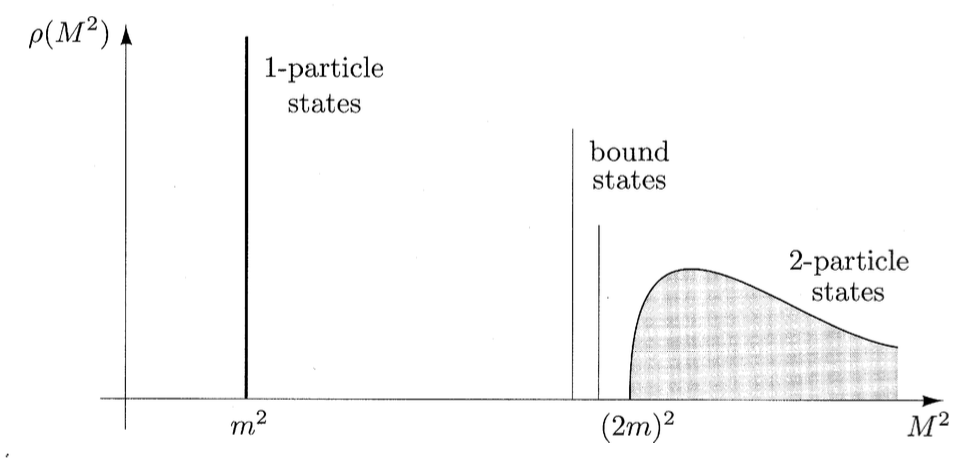
\includegraphics[scale=0.7]{spectral density.png}
  \caption{谱密度图示}
  \label{sd}
\end{figure}
谱密度函数在单粒子质量处有孤立的Delta函数,对于$ M>2m $处是连续的:
\begin{equation}
  \rho\left(M^2\right)=2 \pi \delta\left(M^2-m^2\right) \cdot Z+\left(\text { nothing else until } M^2 \gtrsim(2 m)^2\right)
\end{equation}
Z是由矩阵元平方求和给出的常数,称为场强重整化,m是单粒子的物理质量。\\

对位置空间的关联函数作傅立叶变换,有:
\begin{equation}
  \begin{aligned}
    \int d^4 x e^{i p \cdot x}\langle\Omega|T \phi(x) \phi(0)| \Omega\rangle & =\int_0^{\infty} \frac{d M^2}{2 \pi} \rho\left(M^2\right) \frac{i}{p^2-M^2+i \epsilon} \\
    & =\frac{i Z}{p^2-m^2+i \epsilon}+\int_{\sim 4 m^2}^{\infty} \frac{d M^2}{2 \pi} \rho\left(M^2\right) \frac{i}{p^2-M^2+i \epsilon}
    \end{aligned}
\end{equation}
可以看出,全传播子在物理质量处有极点。
\subsection{LSZ约化公式}
在上节可以看到,动量空间的两点关联函数作为$ p^2 $的解析函数,在单粒子态质量处有如下的极点结构:
\begin{equation}
  \int d^4 x e^{i p \cdot x}\langle\Omega|T \phi(x) \phi(0)| \Omega\rangle \underset{p^2 \rightarrow m^2}{\sim} \frac{i Z}{p^2-m^2+i \epsilon}
  \label{ps}
\end{equation} 
本节将上述结果推广到一般的关联函数,并由此给出关联函数与S矩阵元的关系。考虑一个$ 2\to n $过程,
对其中一个场作傅立叶变换,作为傅立叶变量p的函数具有\eqref{ps}的极点结构。将证明和这些极点关联
起来的单粒子态实际上是渐进态,即以某动量为中心,相隔很远的波包。取n+2个外线粒子在壳极限,可以将
多重极点的系数解释为S矩阵。\\

先对n+2点关联函数其中的一个变量作傅立叶变换,分析下述积分:
\begin{equation}
  \int d^4 x e^{i p \cdot x}\left\langle\Omega\left|T\left\{\phi(x) \phi\left(z_1\right) \phi\left(z_2\right) \cdots\right\}\right| \Omega\right\rangle
\end{equation}
要找出变量$ p^0 $的极点,讲积分拆为三部分:
\begin{equation}
  \int d x^0=\int_{T_{+}}^{\infty} d x^0+\int_{T_{-}}^{T_{+}} d x^0+\int_{-\infty}^{T_{-}} d x^0
\end{equation} 
$ T_+,T_- $分别远大/小于其他的时间$ z_i^0 $。将积分区域分别称为I,II,III,区域II是有界的,
且对$ p^0 $的依赖完全来自解析函数$ \exp(ip^0x^0) $,它的积分对于$ p^0$是解析的。I与III是无界
的,因此有可能产生奇异性。\\

考虑区域I,此处$ \phi(x) $在最前面,插入完备关系(单粒子真空态没有贡献):
\begin{equation}
  \begin{aligned}
    \int_{T_{+}}^{\infty} d x^0 \int d^3 x e^{i p^0 x^0} e^{-i \mathbf{p} \cdot \mathbf{x}} \sum_\lambda \int \frac{d^3 q}{(2 \pi)^3} & \frac{1}{2 E_{\mathbf{q}}(\lambda)}\left\langle\Omega|\phi(x)| \lambda_{\mathbf{q}}\right\rangle \\
    & \times\left\langle\lambda_{\mathbf{q}}\left|T\left\{\phi\left(z_1\right) \phi\left(z_2\right) \cdots\right\}\right| \Omega\right\rangle
    \end{aligned}
\end{equation} 
利用关系\eqref{rela}并插入收敛因子$e^{-\epsilon x^0}  $使得积分良定义,由此有:
\begin{equation}
  \begin{aligned}
    & \sum_\lambda \int_{T_{+}}^{\infty} d x^0 \int \frac{d^3 q}{(2 \pi)^3} \frac{1}{2 E_{\mathbf{q}}(\lambda)} e^{i p^0 x^0} e^{-i q^0 x^0} e^{-\epsilon x^0}\left\langle\Omega|\phi(0)| \lambda_0\right\rangle(2 \pi)^3 \delta^{(3)}(\mathbf{p}-\mathbf{q}) \\
    & \times\left\langle\lambda_{\mathbf{q}}\left|T\left\{\phi\left(z_1\right) \cdots\right\}\right| \Omega\right\rangle \\
    & =\sum_\lambda \frac{1}{2 E_{\mathbf{p}}(\lambda)} \frac{i e^{i\left(p^0-E_{\mathbf{p}}+i \epsilon\right) T_{+}}}{p^0-E_{\mathbf{p}}(\lambda)+i \epsilon}\left\langle\Omega|\phi(0)| \lambda_0\right\rangle\left\langle\lambda_{\mathbf{p}}\left|T\left\{\phi\left(z_1\right) \cdots\right\}\right| \Omega\right\rangle . 
    \end{aligned}
\end{equation} 
可以看出它具有如下极点结构:
\begin{equation}
  \begin{aligned}
    \int d^4 x e^{i p \cdot x}\left\langle\Omega\left|T\left\{\phi(x) \phi\left(z_1\right) \cdots\right\}\right| \Omega\right\rangle \\
    \underset{p^0 \rightarrow+E_{\mathbf{p}}}{\sim} \frac{i}{p^2-m^2+i \epsilon} \sqrt{Z}\left\langle\mathbf{p}\left|T\left\{\phi\left(z_1\right) \cdots\right\}\right| \Omega\right\rangle
    \end{aligned}
\end{equation}
相似地有III的贡献:
\begin{equation}
  \begin{aligned}
    \int d^4 x e^{i p \cdot x}\langle\Omega| & T\left\{\phi(x) \phi\left(z_1\right) \cdots\right\}|\Omega\rangle \\
    & \underset{p^0 \rightarrow-E_{\mathbf{p}}}{\sim}\left\langle\Omega\left|T\left\{\phi\left(z_1\right) \cdots\right\}\right|-\mathbf{p}\right\rangle \sqrt{Z} \frac{i}{p^2-m^2+i \epsilon}
    \end{aligned}
\end{equation}
对剩下的场做傅立叶变换,为防止不同粒子的干涉,取波包模型而非点粒子模型,对于傅立叶变换做出如下改变:
\begin{equation}
  \int d^4 x e^{i p^0 x^0} e^{-i \mathbf{p} \cdot \mathbf{x}} \rightarrow \int \frac{d^3 k}{(2 \pi)^3} \int d^4 x e^{i p^0 x^0} e^{-i \mathbf{k} \cdot \mathbf{x}} \varphi(\mathbf{k})
\end{equation}
$ \varphi(\mathbf{k}) $是表示一个集中在p动量的波包分布。因此,极点结构修正为:
\begin{equation}
  \begin{aligned}
    & \sum_\lambda \int \frac{d^3 k}{(2 \pi)^3} \varphi(\mathbf{k}) \frac{1}{2 E_{\mathbf{k}}(\lambda)} \frac{i}{p^0-E_{\mathbf{k}}(\lambda)+i \epsilon}\left\langle\Omega|\phi(0)| \lambda_0\right\rangle\left\langle\lambda_{\mathbf{k}}\left|T\left\{\phi\left(z_1\right) \cdots\right\}\right| \Omega\right\rangle\\
    & \underset{p^0 \rightarrow+E_{\mathbf{p}}}{\sim} \int \frac{d^3 k}{(2 \pi)^3} \varphi(\mathbf{k}) \frac{i}{\tilde{p}^2-m^2+i \epsilon} \sqrt{Z}\left\langle\mathbf{k}\left|T\left\{\phi\left(z_1\right) \cdots\right\}\right| \Omega\right\rangle
  \end{aligned}
\end{equation} 
此时奇异性从极点变为割线,可以通过缩小$ \varphi(\mathbf{k}) $代表的波包使得割线退化为极点。对关联
函数中所有的变量都做波包型变换:
\begin{equation}
  \left(\prod_i \int \frac{d^3 k_i}{(2 \pi)^3} \int d^4 x_i e^{i \tilde{p}_i \cdot x_i} \varphi_i\left(\mathbf{k}_i\right)\right)\left\langle\Omega\left|T\left\{\phi\left(x_1\right) \phi\left(x_2\right) \cdots\right\}\right| \Omega\right\rangle
\end{equation}
选取$ T_+,T_- $使得波包在I,III区域相隔很远,在x=0处接触。选择粒子1,2处于将来,它们在时序
乘积的前两项,再插入完备算符,此时有:
\begin{equation}
  \begin{aligned}
    & \sum_\lambda \int \frac{d^3 K}{(2 \pi)^3} \frac{1}{2 E_{\mathbf{K}}}\left(\prod_{i=1,2} \int \frac{d^3 k_i}{(2 \pi)^3} \int d^4 x_i e^{i \tilde{p}_i \cdot x_i} \varphi_i\left(\mathbf{k}_i\right)\right) \\
    & \times\left\langle\Omega\left|T\left\{\phi\left(x_1\right) \phi\left(x_2\right)\right\}\right| \lambda_{\mathbf{K}}\right\rangle\left\langle\lambda_{\mathbf{K}}\left|T\left\{\phi\left(x_3\right) \cdots\right\}\right| \Omega\right\rangle
    \end{aligned}
\end{equation}
态$ \lambda_{\mathbf{K}} $被两个相隔很远的波包湮灭,因此它必定对应真空中的两个独立激发,近似有:
\begin{equation}
  \begin{aligned}
    & \sum_\lambda \int \frac{d^3 K}{(2 \pi)^3} \frac{1}{2 E_{\mathbf{K}}}\left\langle\Omega\left|T\left\{\phi\left(x_1\right) \phi\left(x_2\right)\right\}\right| \lambda_{\mathbf{K}}\right\rangle\left\langle\lambda_{\mathbf{K}}\right| \\
    & =\sum_{\lambda_1 \lambda_0} \int \frac{d^3 q_1}{(2 \pi)^3} \frac{1}{2 E_{\mathbf{q}_1}} \int \frac{d^3 q_2}{(2 \pi)^3} \frac{1}{2 E_{\mathbf{q}_2}}\left\langle\Omega\left|\phi\left(x_1\right)\right| \lambda_{\mathbf{q}_1}\right\rangle\left\langle\Omega\left|\phi\left(x_2\right)\right| \lambda_{\mathbf{q}_2}\right\rangle\left\langle\lambda_{\mathbf{q}_1} \lambda_{\mathbf{q}_2}\right|
    \end{aligned}
\end{equation} 
对$ x_1,x_0 $的积分给出上节熟悉的极点结构:
\begin{equation}
  \left(\prod_{i=1,2} \int \frac{d^3 k_i}{(2 \pi)^3} \varphi_i\left(\mathbf{k}_i\right) \frac{i}{\tilde{p}_i^2-m^2+i \epsilon} \cdot \sqrt{Z}\right)\left\langle\mathbf{k}_1 \mathbf{k}_2\left|T\left\{\phi\left(x_3\right) \cdots\right\}\right| \Omega\right\rangle
\end{equation} 
取点粒子极限,并同样地处理其他场,有:
\begin{equation}
  \left(\prod_{i=1,2} \frac{i}{p_i{ }^2-m^2+i \epsilon} \cdot \sqrt{Z}\right)\left(\prod_{i=3, \ldots . .} \frac{i}{p_i{ }^2-m^2+i \epsilon} \cdot \sqrt{Z}\right)_{\text {out }}\left\langle\mathbf{p}_1 \mathbf{p}_2 \mid-\mathbf{p}_3 \cdots\right\rangle_{\mathrm{in}}
\end{equation}
由此可以得出结论:S矩阵元就是对应动量关联函数在多重极点处的系数。综上,LSZ公式为:
\begin{equation}
  \begin{array}{r}
    \prod_1^n \int d^4 x_i e^{i p_i \cdot x_i} \prod_1^m \int d^4 y_j e^{-i k_j \cdot y_j}\left\langle\Omega\left|T\left\{\phi\left(x_1\right) \cdots \phi\left(x_n\right) \phi\left(y_1\right) \cdots \phi\left(y_m\right)\right\}\right| \Omega\right\rangle \\
    \underset{\substack{\text { each } p_i^0 \rightarrow+E_{\mathbf{p}_i} \\
    \text { each } k_j^0 \rightarrow+E_{\mathbf{k}_j}}}{\sim}\left(\prod_{i=1}^n \frac{\sqrt{Z} i}{p_i^2-m^2+i \epsilon}\right)\left(\prod_{j=1}^m \frac{\sqrt{Z} i}{k_j^2-m^2+i \epsilon}\right)\left\langle\mathbf{p}_1 \cdots \mathbf{p}_n|S| \mathbf{k}_1 \cdots \mathbf{k}_m\right\rangle .
    \end{array}
\end{equation}
LSZ公式也解答了为什么计算S矩阵元只考虑了Amputated的图:简单来说,对于自能图我们要求它在粒子质量处
有对应的极点,每条外线的自能图都贡献这样一个极点,刚好就是我们前文所述的极点结构,而S矩阵元是极点的
系数,因此对应了Amputated的图。
\section{Noether定理与local对称性}
  \section{规范场的量子化:QED,非阿贝尔,与凝聚态中的电磁场路径积分}

\section{外场与有效作用量}
\subsection{来自热力学的类比}
考虑一个磁性系统,配分函数以及Helmholtz自由能为:
\begin{equation}
  Z(H)=e^{-\beta F(H)}=\int \mathcal{D} s \exp \left[-\beta \int d x(\mathcal{H}[s]-H s(x))\right]
\end{equation}
$ H $为外加磁场。磁化强度可以通过对Helmholtz自由能求导得到:
\begin{equation*}
  \begin{aligned}
    -\left.\frac{\partial F}{\partial H}\right|_{\beta \text { fixed }} & =\frac{1}{\beta} \frac{\partial}{\partial H} \log Z \\
    & =\frac{1}{Z} \int d x \int \mathcal{D} s s(x) \exp \left[-\beta \int d x(\mathcal{H}[s]-H s)\right] \\
    & =\int d x\langle s(x)\rangle \equiv M .
    \end{aligned}
\end{equation*}
Gibbs自由能 通过Legendre变换得到
\begin{equation*}
  G=f+MH
\end{equation*}
外场可以对Gibbs自由能 求导得到:
\begin{equation}
  \begin{aligned}
    \frac{\partial G}{\partial M} & =\frac{\partial F}{\partial M}+M \frac{\partial H}{\partial M}+H \\
    & =\frac{\partial H}{\partial M} \frac{\partial F}{\partial H}+M \frac{\partial H}{\partial M}+H \\
    & =H
    \end{aligned}
\end{equation}
当$ H=0 $时,Gibbs自由能 取极值,热力学上最稳定的态由$ G(M) $的最小值给出。通过类比,我们也可以在QFT中构造相似的量,为方便仅考虑标量场。
\subsection{有效作用量的引入}
 标量场的生成函数为:
 \begin{equation}
  Z[J]=e^{-i E[J]}=\int \mathcal{D} \phi \exp \left[i \int d^4 x(\mathcal{L}[\phi]+J \phi)\right]
 \end{equation}
 一般而言通常的记号并非$ E(J) $,而是$ W(J) $,后文中可能交替使用两种记号。可以看出$ E(J) $可以类比Helmholtz自由能 ,它的物理意义是
 真空-真空振幅的联通部分。J类比外磁场。之后的讨论中我们假定J是均匀的,通过泛函的一些技巧我们很容易推广到一般的场。\\
 令$ E(J) $对J求泛函导数,有:
 \begin{equation}
  \frac{\delta}{\delta J(x)} E[J]=i \frac{\delta}{\delta J(x)} \log Z=-\frac{\int \mathcal{D} \phi e^{i \int(\mathcal{L}+J \phi)} \phi(x)}{\int \mathcal{D} \phi e^{i \int(\mathcal{L}+J \phi)}}
 \end{equation}  
将上式简记为:
\begin{equation}
  \frac{\delta}{\delta J(x)} E[J]=-\langle\Omega|\phi(x)| \Omega\rangle_J
\end{equation}
等式右侧为有场J时$ \phi $的真空期望。注意到热力学中和外场共轭的物理量也是内场的平均值,因此我们定义:
\begin{equation}
  \phi_{\mathrm{cl}}(x)=\langle\Omega|\phi(x)| \Omega\rangle_J
  \label{defofcf}
\end{equation}
由此定义Gibbs自由能 的QFT类比,即$ E(J) $的Legendre变换
\footnote{在Weinberg等教材中,此处的Legendre变换定义略有不同,并没有取场在源J的真空期望值作为Legendre变换中和J共轭的量
,而是定义$ J_{\phi 人} $为产生期望值为$ \phi^r $的流,再定义Legendre变换:
\begin{equation}
  \Gamma[\phi] \equiv-\int \mathrm{d}^4 x \phi^r(x) J_{\phi r}(x)+W\left[J_\phi\right]
  \label{defofw}
\end{equation}  
后文在计算有效作用量时主要采用了这个定义}
\\
\begin{equation}
  \Gamma\left[\phi_{\mathrm{cl}}\right] \equiv-E[J]-\int d^4 y J(y) \phi_{\mathrm{cl}}(y)
  \label{defofea}
\end{equation} 
对经典场再求泛函导数,有:
\begin{equation}
  \begin{aligned}
    \frac{\delta}{\delta \phi_{\mathrm{cl}}(x)} \Gamma\left[\phi_{\mathrm{cl}}\right] & =-\frac{\delta}{\delta \phi_{\mathrm{cl}}(x)} E[J]-\int d^4 y \frac{\delta J(y)}{\delta \phi_{\mathrm{cl}}(x)} \phi_{\mathrm{cl}}(y)-J(x) \\
    & =-\int d^4 y \frac{\delta J(y)}{\delta \phi_{\mathrm{cl}}(x)} \frac{\delta E[J]}{\delta J(y)}-\int d^4 y \frac{\delta J(y)}{\delta \phi_{\mathrm{cl}}(x)} \phi_{\mathrm{cl}}(y)-J(x) \\
    & =-J(x) .
    \end{aligned}
\end{equation}
热力学和QFT的类比总结如图\ref*{Analog}:\\
\begin{figure}[htp]
  \centering
  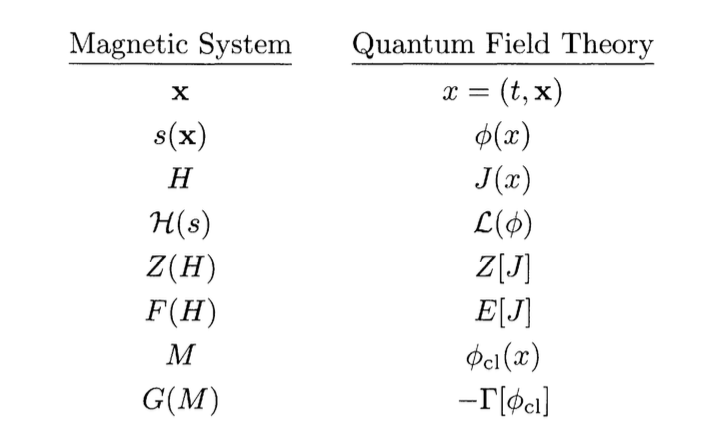
\includegraphics[scale=0.8]{analog.png}
  \caption{热力学与QFT类比}
  \label{Analog}
\end{figure}
很容易看出,当外场为零时,有:
\begin{equation}
  \frac{\delta}{\delta \phi_{\mathrm{cl}}(x)} \Gamma\left[\phi_{\mathrm{cl}}\right]=0
  \label{ec}
\end{equation}
此方程的解就是理论中的稳定构型。对于平移不变的真空态,解是不依赖于x的,但有时也会有额外的解称为瞬子。\\
在此假设考虑的理论中可能的真空态在平移以及Lorentz变换下总是不变的,此时方程变为非常简单的非泛函方程,进一步我们知道
$ \Gamma $是一个广延量,它正比于我们所选取的时空体积:
\begin{equation}
  \Gamma\left[\phi_{\mathrm{cl}}\right]=-(V T) \cdot V_{\mathrm{eff}}\left(\phi_{\mathrm{cl}}\right)
\end{equation} 
系数$ V_{\mathrm{eff}}\left(\phi_{\mathrm{cl}}\right) $称为有效势。$ \Gamma\left[\phi_{\mathrm{cl}}\right] $
取极值的条件简化为$ V_{\mathrm{eff}}\left(\phi_{\mathrm{cl}}\right) $取极值。
\subsection{有效作用量的性质}
先给出结论:我们知道$ Z[J] $是关联函数的生成泛函,而$ \Gamma\left[\phi_{\mathrm{cl}}\right] $ 是单粒子不可约关联函数
的生成泛函。为看出这一点,从两点关联函数算起。
\begin{equation}
  \begin{aligned}
    & \frac{\delta^2 E[J]}{\delta J(x) \delta J(y)}=-\frac{i}{Z} \int \mathcal{D} \phi e^{i \int(\mathcal{L}+J \phi)} \phi(x) \phi(y) \\
    & \quad+\frac{i}{Z^2} \int \mathcal{D} \phi e^{i \int(\mathcal{L}+J \phi)} \phi(x) \cdot \int \mathcal{D} \phi e^{i \int(\mathcal{L}+J \phi)} \phi(y) \\
    &=-i[\langle\phi(x) \phi(y)\rangle-\langle\phi(x)\rangle\langle\phi(y)\rangle] .
    \end{aligned}
\end{equation}
 非连通部分刚好被抵消,对更高阶的泛函导数也有相同的结果(link cluster theorem),因此有:
 \begin{equation}
  \frac{\delta^n E[J]}{\delta J\left(x_1\right) \cdots \delta J\left(x_n\right)}=(i)^{n+1}\left\langle\phi\left(x_1\right) \cdots \phi\left(x_n\right)\right\rangle_{\mathrm{conn}}
 \end{equation}
 现在开始考虑$ \gamma $,对\eqref{ec}求场$ J(y) $的泛函导数有:
 \begin{equation*}
  \frac{\delta}{\delta J(y)} \frac{\delta \Gamma}{\delta \phi_{\mathrm{cl}}(x)}=-\delta(x-y)
 \end{equation*} 
 利用链式法则展开左式:
 \begin{equation}
  \begin{aligned}
    \delta(x-y) & =-\int d^4 z \frac{\delta \phi_{\mathrm{cl}}(z)}{\delta J(y)} \frac{\delta^2 \Gamma}{\delta \phi_{\mathrm{cl}}(z) \delta \phi_{\mathrm{cl}}(x)} \\
    & =\int d^4 z \frac{\delta^2 E}{\delta J(y) \delta J(z)} \frac{\delta^2 \Gamma}{\delta \phi_{\mathrm{cl}}(z) \delta \phi_{\mathrm{cl}}(x)} \\
    & =\left(\frac{\delta^2 E}{\delta J \delta J}\right)_{y z}\left(\frac{\delta^2 \Gamma}{\delta \phi_{\mathrm{cl}} \delta \phi_{\mathrm{cl}}}\right)_{z x}
    \end{aligned}
    \label{2p}
 \end{equation}
 可以看到这两个无限维矩阵互为逆:
 \begin{equation}
  \left(\frac{\delta^2 E}{\delta J \delta J}\right)=\left(\frac{\delta^2 \Gamma}{\delta \phi_{\mathrm{cl}} \delta \phi_{\mathrm{cl}}}\right)^{-1}
 \end{equation}
 已知左式为连通两点关联函数,即传播子,因此右式为传播子的逆。到动量空间可以更容易看出物理意义:
 \begin{equation*}
  \widetilde{D}^{-1}(p)=-i\left(p^2-m^2-M^2\left(p^2\right)\right)
 \end{equation*}
 $ M^2\left(p^2\right) $是自能函数,是所有单粒子不可约两点图的求和。进一步求泛函导数,用链式法则改写求导:
 \begin{equation*}
  \frac{\delta}{\delta J(z)}=\int d^4 w \frac{\delta \phi_{\mathrm{cl}}(w)}{\delta J(z)} \frac{\delta}{\delta \phi_{\mathrm{cl}}(w)}=i \int d^4 w D(z, w) \frac{\delta}{\delta \phi_{\mathrm{cl}}(w)}
 \end{equation*}
 并利用矩阵逆求导的法则:
 \begin{equation*}
  \frac{\partial}{\partial \alpha} M^{-1}(\alpha)=-M^{-1} \frac{\partial M}{\partial \alpha} M^{-1}
 \end{equation*}
 继续对\eqref{2p}求泛函导数,有:
 \begin{equation*}
  \begin{aligned}
    \frac{\delta^3 E[J]}{\delta J_x \delta J_y \delta J_z} & =i \int d^4 w D(z, w) \frac{\delta}{\delta \phi_w^{\mathrm{cl}}}\left(\frac{\delta^2 \Gamma}{\delta \phi_x^{\mathrm{cl}} \delta \phi_y^{\mathrm{cl}}}\right)^{-1} \\
    & =i \int d^4 w D_{z w}(-1) \int d^4 u \int d^4 v\left(-i D_{x u}\right) \frac{\delta^3 \Gamma}{\delta \phi_u^{\mathrm{cl}} \delta \phi_v^{\mathrm{cl}} \delta \phi_w^{\mathrm{cl}}}\left(-i D_{v y}\right)\\
    & =i \int d^4 u d^4 v d^4 w D_{x u} D_{y v} D_{z w} \frac{\delta^3 \Gamma}{\delta \phi_u^{\mathrm{cl}} \delta \phi_v^{\mathrm{cl}} \delta \phi_w^{\mathrm{cl}}}
  \end{aligned}
 \end{equation*}
 \begin{figure}[htp]
  \centering
  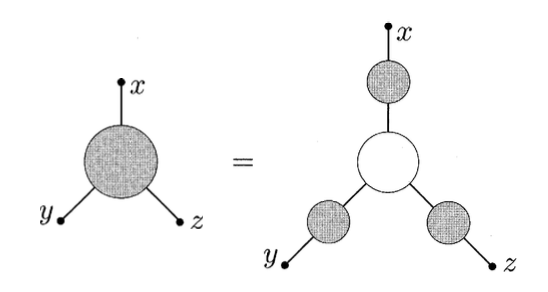
\includegraphics[scale=1]{3DR.png}
  \caption{三点关系的图像表示}
  \label{3DR}
\end{figure}
深灰圈表示连通图的求和,浅灰圈表示量子作用量的三阶泛函导数,可以看出它代表所有完全传播子移除后的连通三点关联函数,
即单粒子不可约三点函数:
\begin{equation*}
  \frac{i \delta^3 \Gamma}{\delta \phi_{\mathrm{cl}}(x) \phi_{\mathrm{cl}}(y) \phi_{\mathrm{cl}}(z)}=\langle\phi(x) \phi(y) \phi(z)\rangle_{1 \mathrm{PI}}
\end{equation*}
继续求导,可以总结出以下关系:
\begin{equation}
  \frac{\delta^n \Gamma\left[\phi_{\mathrm{cl}}\right]}{\delta \phi_{\mathrm{cl}}\left(x_1\right) \cdots \delta \phi_{\mathrm{cl}}\left(x_n\right)}=-i\left\langle\phi\left(x_1\right) \cdots \phi\left(x_n\right)\right\rangle_{1 \mathrm{PI}}
\end{equation}
因此我们得出,量子有效作用量是单粒子不可约关联函数的生成泛函。因此,类比$ W(J) $是所有连通真空-真空图的求和,$ \Gamma[\phi_{cl}] $是所有单粒子不可约
连通图的求和。 \\
若将生成泛函中的经典作用量$ I[\phi] $直接换成量子有效作用量$ \Gamma[\phi] $,则有:
\begin{equation}
  Z_{\Gamma}[j]=e^{W_{\Gamma}[j]}=\int[D \phi(x)] \exp \left[i \Gamma[\phi(x)]+i \int d^4 x j(x) \phi(x)\right]
\end{equation}   
我们将证明,这个生成泛函所代表的真空-真空振幅的连通树图部分给出了原本经典作用量$ I[\phi] $的理论的所有阶贡献。为分离出
树图部分,引入一个常数试图标记不同部分的贡献:
\begin{equation}
  Z_r[j ; \hbar]=e^{w_r[j ; \hbar]}=\int[D \phi(x)] \exp \left[\frac{i}{\hbar}\left(\Gamma[\phi(x)]+\int d^4 x j(x) \phi(x)\right)\right]
\end{equation}
传播子给出贡献$ \hbar $,顶点给出贡献$ \hbar^{-1} $,又拓扑恒等式,圈数$ n_L $、内线数I,顶点数V有关系$ n_L=I-V+1 $,
因此L圈图的贡献正比于$ \hbar^{n_L-1} $,形式上可以有:
\begin{equation}
  W_{\Gamma}[j ; \hbar]=\sum_{n_L=0}^{\infty} \hbar^{n_L-1} \underbrace{W_{\Gamma, n_L}[j]}_{n_L \text { loops }}
\end{equation}     
为分离出树图,形式上取极限$ \hbar\to 0 $,此时圈图贡献趋于零,且路径积分由稳相点主导。 
\subsection{有效作用量的计算}
我们在重整微扰论的框架下,从定义式\eqref{defofea}出发,逐阶计算泛函。首先,照常把拉氏量写为两部分:
\begin{equation}
  \mathcal{L}=\mathcal{L}_1+\delta \mathcal{L}
\end{equation}
把流分为两部分$ J(x)=J_1(x)+\delta J(x) $ ,其中一部分满足如下方程:
\begin{equation}
  \left.\frac{\delta \mathcal{L}_1}{\delta \phi}\right|_{\phi=\phi_{\mathrm{cl}}}+J_1(x)=0
  \label{defofj1}
\end{equation}
而$ \delta J(x) $的取值是的总的流让场的真空期望值仍是$ \phi_{cl}(x) $ 即$ \langle\phi(x)\rangle_J=\phi_{\mathrm{cl}}(x) $\\
现在生成泛函为:
\begin{equation}
  Z[J]=\int \mathcal{D} \phi e^{i \int d^4 x\left(\mathcal{L}_1[\phi]+J_1 \phi\right)} e^{i \int d^4 x(\delta \mathcal{L}[\phi]+\delta J \phi)}
\end{equation}
平移场的定义,取$ \phi(x)=\phi_{\mathrm{cl}}(x)+\eta(x) $ ,指数中的项做幂级数展开:
\begin{equation}
  \begin{aligned}
    \int d^4 x\left(\mathcal{L}_1+J_1 \phi\right) & =\int d^4 x\left(\mathcal{L}_1\left[\phi_{\mathrm{cl}}\right]+J_1 \phi_{\mathrm{cl}}\right)+\int d^4 x \eta(x)\left(\frac{\delta \mathcal{L}_1}{\delta \phi}+J_1\right) \\
    & +\frac{1}{2} \int d^4 x d^4 y \eta(x) \eta(y) \frac{\delta^2 \mathcal{L}_1}{\delta \phi(x) \delta \phi(y)} \\
    & +\frac{1}{3 !} \int d^4 x d^4 y d^4 z \eta(x) \eta(y) \eta(z) \frac{\delta^3 \mathcal{L}_1}{\delta \phi(x) \delta \phi(y) \delta \phi(z)}+\cdots
    \end{aligned}
\end{equation}
一阶项由\eqref{defofj1}直接为零,二阶项给出高斯积分,高阶项视作微扰修正。暂且忽略抵消项与高阶修正,高斯积分给出有效作用量的第一个修正项:
\begin{equation}
  \begin{aligned}
    \int \mathcal{D} \eta & \exp \left[i\left(\int\left(\mathcal{L}_1\left[\phi_{\mathrm{cl}}\right]+J_1 \phi_{\mathrm{cl}}\right)+\frac{1}{2} \int \eta \frac{\delta^2 \mathcal{L}_1}{\delta \phi \delta \phi} \eta\right)\right] \\
    = & \exp \left[i \int\left(\mathcal{L}_1\left[\phi_{\mathrm{cl}}\right]+J_1 \phi_{\mathrm{cl}}\right)\right] \cdot\left(\operatorname{det}\left[-\frac{\delta^2 \mathcal{L}_1}{\delta \phi \delta \phi}\right]\right)^{-1 / 2} .
    \end{aligned}
\end{equation}
高阶项的作用在Feynman图表示中,给出了一系列以$ -i\left(\frac{\delta^2 \mathcal{L}_1}{\delta \phi \delta \phi}\right)^{-1} $ 
作为传播子,高阶项作为顶点的Feynman规则图。\\
考虑抵消项,也在$ \phi_{cl} $处展开,有 
\begin{equation}
  \left(\delta \mathcal{L}\left[\phi_{\mathrm{cl}}\right]+\delta J \phi_{\mathrm{cl}}\right)+\left(\delta \mathcal{L}\left[\phi_{\mathrm{cl}}+\eta\right]-\delta \mathcal{L}\left[\phi_{\mathrm{cl}}\right]+\delta J \eta\right)
\end{equation}
第二项Taylor展开后也给出Feynman图修正,第一项是一个常数。总结,有效作用量为:
\begin{equation}
  \begin{aligned}
    \Gamma\left[\phi_{\mathrm{cl}}\right]= & \int d^4 x \mathcal{L}_1\left[\phi_{\mathrm{cl}}\right]+\frac{i}{2} \log \operatorname{det}\left[-\frac{\delta^2 \mathcal{L}_1}{\delta \phi \delta \phi}\right] \\
    & -i \cdot(\text { connected diagrams })+\int d^4 x \delta \mathcal{L}\left[\phi_{\mathrm{cl}}\right]
    \end{aligned}
\end{equation}
上述连通图都是真空-真空图,至少也是两圈图,因此最低阶修正就是泛函行列式。上面的构造中比正常的重整化多了一个抵消项:$ \delta J $,它由
下述方法给出:\\
首先在头阶项有关系$ \langle\phi\rangle=\phi_{\mathrm{cl}} $,此等式会因为Feynman图给出的修正而不成立,且贡献都来自于
“蝌蚪”图,他们刚好可以由$ \delta J\eta $项抵消是的等式依然成立。在实际操纵中我们直接忽略连通单粒子不可约单点图,因为刚好被
$ \delta J\eta $抵消。
\subsection{有效作用量的对称性}
虽然不总是这样, 但在某些情况下, 作用量$ I[\phi] $ 的对称性自动地也是有效作用量的$ \Gamma[\phi] $ 的对称性。除非我们能够证明附加于作用量的对称性也适用于有效作用量, 否则我们在建立理论的可重 整性时会遇到问题。\\
为此没我们研究一种重要的对称性,它由如下无限小变换生成:
\begin{equation}
  \chi^n(x) \rightarrow \chi^n(x)+\epsilon F^n[x ; \chi]
\end{equation}
假定测度和作用量在变换下都不变:
\begin{equation}
  \begin{aligned}
    I[\chi+\epsilon F] & =I[\chi] \\
    \prod_{n, x} \mathrm{~d}\left(\chi^n(x)+\epsilon F[x ; \chi]\right) & =\prod_{n, x} \mathrm{~d} \chi^n(x)
    \end{aligned}
\end{equation}
此时生成泛函为:
\begin{equation}
  \begin{aligned}
    Z[J]= & \int\left[\prod_{n, x} \mathrm{~d}\left(\chi^n(x)+\epsilon F^n[x ; \chi]\right)\right] \\
    & \times \exp \left\{\mathrm{i} I[\chi+\epsilon F]+\mathrm{i} \int \mathrm{d}^4 x\left(\chi^n(x)+\epsilon F^n[x ; \chi]\right) J_n(x)\right\} \\
    = & \int\left[\prod_{n, x} \mathrm{~d} \chi^n(x)\right] \exp \left\{\mathrm{i} I[\chi]+\mathrm{i} \int \mathrm{d}^4 x\left(\chi^n(x)+\epsilon F^n[x ; \chi]\right) J_n(x)\right\} \\
    = & Z[J]+\mathrm{i} \epsilon \int\left(\prod_{n, x} \mathrm{~d} \chi^n(x)\right) \int F^n(y ; \chi) J_n(y) \mathrm{d}^4 y \\
    & \times \exp \left\{\mathrm{i} I[\chi]+\mathrm{i} \int \mathrm{d}^4 x \chi^n(x) J_n(x)\right\}
    \end{aligned}
\end{equation}
上式中Taylor展开了指数项。因此:
\begin{equation}
  \int \mathrm{d}^4 y\left\langle F^n(y)\right\rangle_J J_n(y)=0
\end{equation}
回忆起在此定义下流由此式给出:
\begin{equation}
  J_{n, \chi}(y)=-\frac{\delta \Gamma[\chi]}{\delta \chi^n(y)}
\end{equation}
因此有:
\begin{equation}
  0=\int \mathrm{d}^4 y\left\langle F^n(y)\right\rangle_{J_\chi} \frac{\delta \Gamma[\chi]}{\delta \chi^n(y)}
\end{equation}
也即$ \Gamma[\chi] $在无限小变换
\begin{equation}
  \chi^n(y) \rightarrow \chi^n(y)+\epsilon\left\langle F^n(y)\right\rangle_{J_\chi}
\end{equation} 
下不变,这样的对称性调教被称为Slavnov-Taylor恒等式。若我们出发的无限小变换时线性变换那两者时相同的。
\section{量子Goldstone定理}

QFT中的Goldstone定理证明与经典场类似,只不过势能换成有效势。为说明这一点,需要引入一些关于有效作用量的结论.
\subsection{寻找真空}
我们知道,量子有效作用量在场的真空期望值处取极值:
\begin{equation}
  \left(\frac{\delta \Gamma[\phi]}{\delta \phi(x)}\right)_{\phi=\langle\Omega|\phi| \Omega\rangle}=0
\end{equation}
为找出真空态$ |\Psi> $,它需要使得哈密顿量期望值最小,并且对场的期望值给出上述极值条件的解,还要满足归一性,利用Lagrange乘数法
求解这个约束极值问题,可以转化为最小化以下的量:
\begin{equation}
  \langle\Psi|H| \Psi\rangle-A\langle\Psi \mid \Psi\rangle-\int d^3 x B(\mathbf{x})\langle\Psi|\phi(\mathbf{x})| \Psi\rangle
\end{equation} 
对量子态变分取极值,给出条件:
\begin{equation}
  H|\Psi\rangle=A|\Psi\rangle+\int d^3 x B(\mathbf{x}) \phi(\mathbf{x})|\Psi\rangle
\end{equation}
\begin{equation}
  \left(H-\int d^3 x J(\mathbf{x}) \phi(\mathbf{x})\right)\left|\Psi_J\right\rangle=E[J]\left|\Psi_J\right\rangle
\end{equation}
原则上A、B的值也需要求极值得出,最终结果以泛函的关系依赖于场的期望值$ \phi_0{x0} $,但可以通过一种取巧的方式找到A、B。\\
考虑含流哈密顿量的基态本征方程:
\begin{equation}
  \left(H-\int d^3 x J(\mathbf{x}) \phi(\mathbf{x})\right)\left|\Psi_J\right\rangle=E[J]\left|\Psi_J\right\rangle
\end{equation}
若取$ B=J_0:=J_{\phi_0}, A=E\left[J_{\phi_0}\right] $,则$ \left|\Psi_J\right\rangle $ 满足约束条件且能量取极值。\\
为得到有效作用量与能量的关系,考虑这样一个过程:$ -\infty\to +\infty $过程中,逐渐光滑地打开源,并维持恒定的$ J(\vec{x}) $时间T,最后再光滑地撤去源。\\
真空-真空振幅会积累一个相因子:
\begin{equation}
  \langle\Omega, \infty \mid \Omega,-\infty\rangle_J=\exp (-i E[J] T)
\end{equation}
于是有关系:$ W[J]=-E[J] T $。回到没有外源的原本理论,它的真空态由下列方程给出:
\begin{equation}
  \begin{aligned}
    H\left|\Psi_{J_0}\right\rangle&=\left(E[J_0]+\int d^3 x J_0(\mathbf{x}) \phi_0(\mathbf{x})\right)\left|\Psi_{J_0}\right\rangle\\
    &=\frac{1}{T}\left(-W\left[J_0\right]+\int d^4 x J_0(x) \phi_0(x)\right)\left|\Psi_{J_0}\right\rangle\\
    &=-\frac{\Gamma\left[\phi_0\right]}{T}\left|\Psi_{J_0}\right\rangle
  \end{aligned}
\end{equation}
也就是说,对于期望值为$ \phi_0 $的场构型的态,它的能量与该场构型对应的量子作用量只相差一个负系数。满足极值条件的场构型
中,是的量子作用量最大值的就对应能量的最低点,即真空态。 \\

我们总希望真空仍就具有Poincare群的对称性,因此场的期待值是一个常数,从而量子作用量的展开中含导数项的都为零,只剩下了
$ V_{eff} $称为有效势$ \Gamma\left[\phi_0\right]=-V T V_{\mathrm{eff}}\left(\phi_0\right) $,此时寻求真空
就变成了寻求有效势的极值,而在最低阶近似下有效势就是拉氏量中的经典势。
\subsection{简并真空}
经典中基态简并,系统由于历史或者各种微扰处于某个确定的破缺对称性的基态是容易理解的,但由于量子
系统的线性可加,需要额外的论述。事实上,只有无限大的量子系统才能有自发对称破缺。\\

考虑最简单的一个对称性,反射对称性:$ \phi \rightarrow-\phi $ ,此时基态二重简并,$ |\mathrm{VAC},+\rangle,|\mathrm{VAC},-\rangle $
都是对称破缺的基态,但$ |\mathrm{VAC},\rangle\pm |\mathrm{VAC},+\rangle $ 仍具有对称性。 
假设哈密顿量的真空矩阵元为:
\begin{equation}
  \begin{aligned}
    & \langle\mathrm{VAC},+|H| \mathrm{VAC},+\rangle=\langle\mathrm{VAC},-|H| \mathrm{VAC},-\rangle \equiv a \\
    & \langle\mathrm{VAC},+|H| \text { VAC },-\rangle=\langle\mathrm{VAC},-|H| \mathrm{VAC},+\rangle \equiv b
    \end{aligned}
\end{equation}
此时l两者的线性组合才是本征态,且对称不变。真空态之间的隧穿概率可以由下式得出:
\begin{equation}
  \left\langle\Omega_{+}\left|e^{i H t}\right| \Omega_{-}\right\rangle \approx e^{-S_E}=e^{-V \int_0^t \mathcal{L}_E\left(\phi_{\mathrm{cl}}\right) d t}
\end{equation}
$ S_E $为wick转动以后的欧几里得作用量,上述过程取了鞍点近似,积分一般为一有限值,因此空间
体积将指数压缩隧穿概率。 此时两个$ \pm $线性组合态高度简并。考虑破坏对称性的微扰,它将解除
简并,使得$ \mathrm{VAC},\pm\rangle $成为本征值不同的本征态,物理真空具体是谁取决于微扰
本身,但只要它比原本的哈密顿量小很多就不重要。当系统体积有限时,微扰对矩阵元的贡献远小于“隧穿”
对非对角元的贡献,此时基态仍是对称的叠加态,也就是说没有发生对称破缺。 
\subsection{量子Goldstone定理的证明}  
\paragraph*{Proof\: 1}
第一个证明与之前经典的情况几乎完全一致,只需补充几个小细节。我们假设作用量以及测度再一个连续
对称变化下都不变,它的代表,无限小变换时线性的:
\begin{equation}
  \phi_n(x) \rightarrow \phi_n(x)+\mathrm{i} \epsilon \sum_m t_{n m} \phi_m(x)
\end{equation}
由之前的论证,作用量线性的对称性在量子作用量中仍然保持,因此有关系:
\begin{equation*}
  \sum_{n, m} \int \frac{\delta \Gamma[\phi]}{\delta \phi_n(x)} t_{n m} \phi_m(x) \mathrm{d}^4 x=0
\end{equation*}
再考虑平移不变理论,作用量的形式为$ \Gamma[\phi]=-\mathscr{V} V(\phi) $,不变条件可以改写为:
\begin{equation*}
  \sum_{n, m} \frac{\partial V(\phi)}{\partial \phi_n} t_{n m} \phi_m=0
\end{equation*}
再次对场球道,并且利用极值条件,给出关系:
\begin{equation*}
  \left.\sum_{n, m} \frac{\partial^2 V(\phi)}{\partial \phi_n \partial \phi_{\ell}}\right|_{\phi=\bar{\phi}} t_{n m} \bar{\phi}_m=0
\end{equation*}
在经典的情况中,势能二阶导矩阵的本征值直接被认为是质量。有效势的二阶导如有效作用量节
所述,是单粒子不可约两点图之和,直接与动量空间的完全传播子的导数联系:
\begin{equation*}
  \frac{\partial^2 V(\phi)}{\partial \phi_n \partial \phi_{\ell}}=\Delta_{n \ell}^{-1}(0)
\end{equation*}
因此方程改写为:
\begin{equation*}
  \sum_{n, m} \Delta_{n \ell}^{-1}(0) t_{n m} \bar{\phi}_m=0
\end{equation*}
当对称性破缺时,$ \sum_m t_{n m} \bar{\phi}_m $不为零,此时它是$ \Delta_{n \ell}^{-1}(0) $
本征值为零的本征矢,若对角化,$ \phi_{Gm}=U_{nm}\phi_{m} $,$U_{mn}$为使得矩阵对角化的变换
,n取为零本征值对应的下标。这意味着$ \Delta_{n \ell}^{-1}(q) $在$ q^2=0 $处有一极点,
因此无质量。\\

为看出Goldstone粒子属于洛伦兹群的哪个表示,我们先假设场$ \phi_\alpha $对应
表示D,于是有$ \phi_\alpha^{\prime}=D_{\alpha \beta}(\Lambda) \phi_\beta $。Goldstone子
与原本场的线性关系可能让人误以为他们对应相同的表示,但U在Lorentz变化下并不平庸,为看出这一点,
传播子的倒数按照$ D^{-1}\otimes D^{-1} $变换 ,对角化后的矩阵为Lorentz标量矩阵,因此变换矩阵
按照$ D^{-1} $变换,刚好抵消的原本场的变换,因此Goldstone粒子是零自旋玻色子。
\paragraph*{Proof\: 2}
任何连续对称性都给出一个守恒流$ J^{\mu} $,以及相应的守恒荷Q,并且这个Q诱导对应的对称变换:
\begin{equation*}
  Q=\int \mathrm{d}^3 x J^0(\mathbf{x}, 0)
\end{equation*} 
\begin{equation*}
  \left[Q, \phi_n(x)\right]=-\sum_m t_{n m} \phi_m(x)
\end{equation*}
上述算符关系不受自发对称性破缺的影响。现在考察流和场的对易子的真空期望值,并对中间态求和,有:
\begin{equation}
  \left\langle\left[J^\lambda(y), \phi_n(x)\right]\right\rangle_{\mathrm{VAC}}=(2 \pi)^{-3} \int \mathrm{d}^4 p\left[\rho_n^\lambda(p) \mathrm{e}^{\mathrm{i} p \cdot(y-x)}-\tilde{\rho}_n^\lambda(p) \mathrm{e}^{\mathrm{i} p \cdot(x-y)}\right]
\end{equation}
其中利用平移不变形,以及插入完备关系定义了:
\begin{equation}
  \begin{aligned}
    & (2 \pi)^{-3} \mathrm{i} \rho_n^\lambda(p)=\sum_N\left\langle\operatorname{VAC}\left|J^\lambda(0)\right| N\right\rangle\left\langle N\left|\phi_n(0)\right| \mathrm{VAC}\right\rangle \delta^4\left(p-p_N\right), \\
    & (2 \pi)^{-3} \mathrm{i} \tilde{\rho}_n^\lambda(p)=\sum_N\left\langle\operatorname{VAC}\left|\phi_n(0)\right| N\right\rangle\left\langle N\left|J^\lambda(0)\right| \operatorname{VAC}\right\rangle \delta^4\left(p-p_N\right) .
    \end{aligned}
\end{equation}
对N的求和表示对所有离散的指标求和以及对连续指标的积分。由于$ \rho $是动量四矢的函数,且自身
有一个Lorentz矢量指标,因此正比于$ p^\mu $,而插入完备集中的态能量总是正定的,因此也正比
于能量的阶梯函数,即:
\begin{equation}
  \begin{aligned}
    & \rho_n^\lambda(p)=p^\lambda \rho_n\left(-p^2\right) \theta\left(p^0\right) \\
    & \tilde{\rho}_n^\lambda(p)=p^\lambda \tilde{\rho}_n\left(-p^2\right) \theta\left(p^0\right)
    \end{aligned}
\end{equation}  
真空期望可以改写为:
\begin{equation}
  \begin{aligned}
    \left\langle\left[J^\lambda(y), \phi_n(x)\right]\right\rangle_{\mathrm{VAC}}= & \frac{\partial}{\partial y_\lambda} \int \mathrm{d} \mu^2\left[\rho_n\left(\mu^2\right) \Delta_{+}\left(y-x ; \mu^2\right)\right. \\
    & \left.+\tilde{\rho}_n\left(\mu^2\right) \Delta_{+}\left(x-y ; \mu^2\right)\right]
    \end{aligned}
\end{equation}
其中:$  \Delta_{+}\left(z ; \mu^2\right)=(2 \pi)^{-3} \int \mathrm{d}^4 p \theta\left(p^0\right) \delta\left(p^2+\mu^2\right) \mathrm{e}^{\mathrm{i} p \cdot z}$。\\

当$ z^2>0 $时,Lorentz不变形要求$ \Delta_{+}\left(z ; \mu^2\right) $仅能依赖于$ z^2、\mu^2 $。
因此$ \Delta_{+}\left(z ; \mu^2\right) $关于$ (x-y) $在类空时是偶函数,此时:
\begin{equation}
  \left\langle\left[J^\lambda(y), \phi_n(x)\right]\right\rangle_{\mathrm{VAC}}=\frac{\partial}{\partial y_\lambda} \int \mathrm{d} \mu^2\left[\rho_n\left(\mu^2\right)+\tilde{\rho}_n\left(\mu^2\right)\right] \Delta_{+}\left(y-x ; \mu^2\right)
\end{equation}    
由因果关系,类空对易子必为零给出条件:
\begin{equation}
  \rho_n\left(\mu^2\right)=-\tilde{\rho}_n\left(\mu^2\right)
\end{equation}
而对于一般的x,y,代入上式给出:
\begin{equation}
  \left\langle\left[J^\lambda(y), \phi_n(x)\right]\right\rangle_{\mathrm{VAC}}=\frac{\partial}{\partial y_\lambda} \int \mathrm{d} \mu^2 \rho_n\left(\mu^2\right)\left[\Delta_{+}\left(y-x ; \mu^2\right)-\Delta_{+}\left(x-y ; \mu^2\right)\right]
\end{equation}
为利用流守恒条件,两边同时再对$ Y^\lambda $求导,利用性质:
\begin{equation*}
  \left(\square_y-\mu^2\right) \Delta_{+}\left(y-x ; \mu^2\right)=0
\end{equation*} 
于是,对于任意的x和y,有:
\begin{equation}
  0=\int \mathrm{d} \mu^2 \mu^2 \rho_n\left(\mu^2\right)\left[\Delta_{+}\left(y-x ; \mu^2\right)-\Delta_{+}\left(x-y ; \mu^2\right)\right]
\end{equation}
只能有:
\begin{equation}
  \mu^2 \rho_n\left(\mu^2\right)=0
\end{equation}
此方程的解要么为$ rho_n\left(\mu^2\right)=0 $,要么为$ rho_n\left(\mu^2\right)\propto\delta(\mu^2) $。
我们将看到,对于对称破缺情况,只能为后者。
令$ \lambda=0,x^0=y^0=0 $,则有:
\begin{equation}
  \begin{aligned}
    \left\langle\left[J^0(\mathbf{y}, t), \phi_n(\mathbf{x}, t)\right]\right\rangle_{\text {VAC }}= & 2 \mathrm{i}(2 \pi)^{-3} \int \mathrm{d} \mu^2 \rho_n\left(\mu^2\right) \\
    & \times \int \mathrm{d}^4 p \sqrt{\mathbf{p}^2+\mu^2} \mathrm{e}^{\mathrm{i} \mathbf{p} \cdot(\mathbf{y}-\mathbf{x})} \theta(p_0)\delta\left(p^2+\mu^2\right) \\
    = & \mathrm{i} \delta^3(\mathbf{y}-\mathbf{x}) \int \mathrm{d} \mu^2 \rho_n\left(\mu^2\right) .
    \end{aligned}
\end{equation} 
其中用到了公式:$ \int_{-\infty}^{+\infty} d k^0 \delta\left(k^2+m^2\right) \theta\left(k^0\right)=\frac{1}{2 \omega} $ 。
对y空间积分,利用荷Q生成了这个对称变换,给出:
\begin{equation}
  -\sum_m t_{n m}\left\langle\phi_m\right\rangle_{\mathrm{VAC}}=\mathrm{i} \int \mathrm{d} \mu^2 \rho_n\left(\mu^2\right)
\end{equation}
仅当
\begin{equation}
  \rho_n\left(\mu^2\right)=\mathrm{i} \delta\left(\mu^2\right) \sum_m t_{n m}\left\langle\phi_m(0)\right\rangle_{\mathrm{VAC}}
\end{equation}
可以看出,对称破缺时,$ \rho_n\left(\mu^2\right) $不能为零,但正比于$ \delta\left(\mu^2\right) $的项职能出现在无质量粒子
的理论中,而且必须是单粒子态,因为多粒子态会给出连续的贡献。态$  \phi_n(0)|\mathrm{VAC}\rangle$是旋转
不变的\footnote{这似乎依赖$ \phi $是标量场 },因此呢只有螺旋度为零的态对$ \left\langle N\left|\phi_n(0)\right| \text { VAC }\right\rangle $
有贡献,同时只有内禀宇称以及内部量子数同$ J_0 $相同的态N对$ \left\langle V A C\left|J^0\right| N\right\rangle $有贡献,
因此呢Goldstone粒子是一个自旋为零的无质量粒子,且与$ J_0 $有相同的宇称以及内部量子数。     
\chapter{张量网络}

\bibliographystyle{IEEEtran}
\bibliography{Ref}
\end{document}
